%% Elementary Theory of the Reals

\def\FIXX#1{\symbolfootnote[2]{\tt [#1]}}


\section{Introduction}

This paper contains a collection of problems
in geometry.  Each problem can in fact be expressed in 
Tarksi's language of the real numbers.  There are decision
procedures to decide 
the truth of
any statement expressed in Tarski's language.  In this
sense, every problem in this collection is elementary.



\subsection{Flyspeck}

The Kepler conjecture asserts that no packing of congruent
balls in three dimensions has density greater than $\pi/\sqrt{18}$.
This density is achieved by various packings, including the
face-centered cubic packing.

A long computer-assisted proof of the Kepler conjecture appears
in \cite{DCG}.  The aim of an project called {\it Flyspeck} is
to give a complete formalization of this proof of the Kepler
conjecture.  (The name {\it Flyspeck} comes from the acronym {\it FPK},
for the {\it Formal Proof of the Kepler} conjecture.)

This paper is a contribution to the Flyspeck project.  The problems
in this collection were extracted from the proof of the Kepler
conjecture.   All of the extracted problems share certain 
features.  They can all be expressed as statements in Tarski's
language of the real numbers.  They are all statements
about the geometry of configurations in three dimensional Euclidean
space.  They can all be expressed with a small number of quantifiers.

\subsection{Complexity}

What is meant by a {\it small} number of quantifiers?  Most of
the statements are about configurations of points.  Each point
is described by three coordinates, and hence three quantifiers.
In addition to the quantifiers that specify the coordinates there
may be a few additional quantifiers that specify the internal
relations among points.  For example, many statements assert that
two affine spaces intersect, and this is expressed through existential
quantifiers.
  
The collection is generally
arranged in order of increasing number of points.  This ordering
is not strict, because we have also tried to order the results
according to logical dependence, and to group together results 
that bear an affinity to one another.  The largest section of
the collection deals with five-point configurations.  
There is a smaller group of results about six-point configurations,
and then just a few results that involve seven or eight points.

From the point of view of quantifier elimination over the real
numbers, a configuration
of eight points is a daunting problem.  It involves 24 quantifiers
for the coordinates,  together with the additional
quantifiers asserting the internal relations among the points.



However, these problems are all rather simple from a geometrical
point of view.  Eight points, for example, can be viewed as the
vertices of two tetrahedra in Euclidean space.    There is only
one result in this collection that concerns eight points, and
it is the assertion that two tetrahedra, subject to various
simple constraints, have disjoint interiors.  It is a completely
trivial
matter to give a direct geometrical proof of this result.


\subsection{Methods of Proof}

Each statement in this collection is accompoanied by a proof.
In keeping with the elementary nature of the statements, 
we have generally tried to restrict our methods of proof to
elementary arguments.  We avoid quoting results from external
sources to make this collection self-contained.

As a rule, we avoid limits, calculus, analysis, and measure theory.
There are rare exceptions, where we look at the sign of derivative in a proof
to determine whether a function is increasing. 
There are a few compactness arguments implicit in some
of the proofs, where we move some of the points in a configuration
until a constraint is satisfied.

Non-elementary functions have been avoided as a rule.  A few
arguments are based on consideration of angle, which are defined
in terms of point configurations by means of an inverse trigonometric
function.  (See Section~\ref{sec:trig}.)  However, as we point
out in that section, the inverse trigonometric functions can be
eliminated from equations that are linear in the angle, by making
suitable use of trigonometric addition formulas.  Thus, the only purpose of
the inverse trigonometric functions is to make the
proofs more legible.

A few results elementary results in \cite{DCG} were established
by computer.  In a few cases, we have retained a computer-assisted
proof.  Each computer-verified inequality carries a nine-digit 
identification
number \calc{123456789} that helps to locate the computer code
that specifies the inequality and that performs the verification.

\subsection{Formalization}

Although proofs have been provided for all the results, it is
my hope that other proofs might be found that are better adapted
to formalization.  In the best of all possible
worlds, we might hope for
algorithms that entirely automate the proofs in this collection.
This collection is not altogether different from the large collection
of problems in geometry that have been successfully automated
by Wu's method. 

After all, a quick glance at the problems shows that these are
mostly simple results about incidence in affine geometry, convexity, cones,
and the circumradius.  If such a collection lies beyond
the limits of automation, then this does not bode well for 
the general discipline of automated theorem proving.  That then
is the hope and challenge of this piece of the flyspeck project:
to find algorithms to automate the proofs in this collection.


Some general proof methods have been suggested
in a companion article \cite{method}.  These proposed methods include
quantifier elimination, energy minimization of tensegrities,
sums-of-squares decompositions, and global optimization.  


\subsection{Stick Figures}

Some of the results are accompanied by figures.  Some of these
figures are called ``stick figures.'' These are highly schematicized
two dimensional representations of the configurations.

In a stick figure, there is generally one point, called the
base point.  (As a general rule, it is the point called $v_0$ in
the statement of the result.) 

The base point does not appear in the stick figure.  Rather, it
is the point of perspective, from which every other point is viewed.
More precisely, let $S=\{v_0,v_1,\ldots,v_k\}$ be a set of points
in $\ring{R}^3$.  Assume that there is a plane $P$ that separates
$v_0$ from all the points $\{v_1,\ldots,v_k\}$.  Then each point
$v_j$, for $j\ne 0$, gives a segment from $v_j$ to $v_0$ that intersects
$P$ in a point $\bar v_j$.  The stick figure draws the points
$\{\bar v_1,\ldots ,\bar v_k\}\subset P$ in the plane $P$.
A line segment from $v_i$ to $v_j$, with $i,j>0$, is represented by a
line segment from $\bar v_i$ to $\bar v_j$ in the stick figure.
A line segment from $v_i$ to $v_0$ degenerates to a single point $\bar v_i$
in the stick figure.

The stick figures are not drawn to scale.  Rather they give
a quick and dirty schematic representation of the points of a configuration
in a way that is represents the primary incidence relations.
In fact, in general it would be impossible to draw the stick figures
to scale, because many of the results assert that the given
configurations do not exist!

A stick figure should be imagined with the viewer located to one
side of $P$ and the base point $v_0$ to the other side of $P$.  Thus,
the viewer sits in front of the printed page, and the
the base point is located {\it behind} it.  With
this perspective in mind, 
when a segment $\bar v_i$ to $\bar v_j$ is shown as
passing over a segment $\bar v_k$ to $\bar v_\ell$, this is intended
to convey the geometric fact that the segment $v_k$ to $v_\ell$ meets
the triangular convex hull of the three points $v_i,v_j,v_0$.  That
is, the viewer perceives the segment $v_i$ to $v_j$ as lying in front
of the segment $v_k$ to $v_\ell$.

There are certain conventions for representing various length constraints.
Various segments are constrained to have lengths between $2$ and $2.51$
(or some constant close to $2.51$).\footnote{The number $2.51$ appears
throughout this collection.  It appears here, because it appers throughout
the proof of the Kepler conjecture.  It would be more natural to
rewrite all of the results so that the constants that appear are
optimal for the given configurations.  This would give
the results in this collection a more natural and definitive
form.  However, I fear that this would complicate some of
the proofs.  For that reason the results are left in their
current form.}  When a segment $v_j$ to $v_0$
has unspecified length the corresponding vertex $\bar v_j$ is represented
as a black dot.  If $v_j$ to $v_0$ has length between $2$ and $2.51$
(or thereabouts), then $\bar v_j$ is represented as a unfilled dot.
If $v_j$ to $v_0$ has length between $2.51$ and $\sqrt8$ (or
thereabouts), then $\bar v_j$ is represented as a crossed dot.

A segment $v_i$ to $v_j$ in the approximate range $[2,2.51]$ is marked with
an unfilled segment $\bar v_i$ to $\bar v_j$.  In the approximate
range $[2.51,\sqrt8]$, the segment $\bar v_i$ to $\bar v_j$ is marked
with an $X$.  There are no markings on segments of unknown length
constraints.


\pdffig{stick_template}{stick}{some features of stick figures}


\subsection{Usage Notes}

By extracting various results from the proof of the Kepler conjecture,
there is danger that their original context might be forgotten.
For that reason, many of the results are accompanied by usage
notes that indicate the purpose of the result in relation to \cite{DCG}.

The collection of problems and their proofs are completely independent
of these usage notes.   

\section{Functions}

\subsection{Definitions}\label{def:poly:tarski}

We define the following polynomials.
$$
\begin{array}{lll}
\ups(x,y,z) &= -x^2 - y^2 - z^2 + 2 x y + 2 y z + 2 z x.\\
\\
\rho(x_{ij}) &=
   -x_{14}^2 x_{23}^2 - x_{13}^2x_{24}^2 - x_{12}^2 x_{34}^2   \\
 &\quad +2x_{12}x_{14}x_{23}x_{34} + 2x_{12}x_{13}x_{24}x_{34} 
     + 2 x_{13} x_{14}x_{23}x_{24}\\
\\
 \chi(x_{ij}) &= \chi(x_{12},x_{13},x_{14},x_{34},x_{24},x_{23})\\
     &=
      x_{13} x_{23} x_{24} + x_{14} x_{23} x_{24}  + 
      x_{12} x_{23} x_{34} + x_{14} x_{23} x_{34} + x_{12} x_{24} x_{34}\\ 
      &\quad + x_{13} x_{24} x_{34} - 
      2 x_{23} x_{24} x_{34} - x_{12} x_{34}^2 
      - x_{14} x_{23}^2 - x_{13} x_{24}^2\\
   % &= x_1 x_4 x_5 + x_1 x_6 x_4 + x_2 x_6 x_5 + x_2 x_4 x_5 + x_5 x_3 x_6 \\
   %&\quad+ x_3 x_4 x_6 - 2 x_5 x_6 x_4 - x_1 x_4^2 - x_2 x_5^2 - x_3 x_6^2.\\
\\
\Delta(x_{ij}) &= 
   -x_{12} x_{13} x_{23} - x_{12} x_{14} x_{24} - x_{13} x_{14} x_{34} 
    - x_{23} x_{24} x_{34}\\
    &\quad + x_{12} x_{34} (-x_{12} + x_{13} + x_{14} + x_{23} + x_{24} - x_{34}) \\
  &\quad + x_{13} x_{24} (x_{12} - x_{13} + x_{14} + x_{23} - x_{24} + x_{34})\\
    &\quad + x_{14} x_{23} (x_{12} + x_{13} - x_{14} - x_{23} + x_{24} + x_{34})\\
   %x_1 x_4 (- x_1+x_2+x_3- x_4+x_5+x_6)+\\&
   %         x_2 x_5 (x_1- x_2+x_3+x_4- x_5+x_6)
   %         +x_3 x_6 (x_1+x_2- x_3+x_4+x_5- x_6)
   %         - \\&x_2 x_3 x_4- x_1 x_3 x_5- x_1 x_2 x_6- x_4 x_5 x_6\\
\end{array}
    \tlabel{def:chi}\usage{DCG-[5.14]{ def:chi}}
\tlabel{def:delta}
\tlabel{def:ups}
   \index{ZZwchi@$\chi$}
$$
\noindent
The polynomial $\chi$ has less symmetry that $\rho$ and $\Delta$.  For that
reason, we need to take greater care with $\chi$ about the order in which the variables are
listed as arguments.  Note that the last three arguments of
$\chi$ contain the three variables $x_{ij}$ whose indices $ij$ satisfy $i\ne 1\ne j$.
Also, the $i$th and $(i+3)$rd argument of $\chi$ contain distinct indices.

We write $\Delta_{(ij)}(x_{ij})$ for the partial derivative of $\Delta$
with respect to $x_{ij}$.



\begin{definition}\tlabel{def:eta}\usage{DCG-[4.20]{ def:eta}}
\index{circumradius}
%
 \index{Zeta@$\eta$}
Let $\eta$ be defined as
	$$\eta(x,y,z) = x y z/\sqrt{\ups(x^2,y^2,z^2)}.$$
Also, if $v_1,v_2,v_3\in\ring{R}^3$, set
   $\eta_V(v_1,v_2,v_3) =\eta(|v_1-v_2|,|v_2-v_3|,|v_1-v_3|)$.
\end{definition}

\begin{definition}\tlabel{def:CM}
\index{Cayley-Menger}
\index{CM}
If $v_1,\ldots,v_n\in\ring{R}^k$, define
the Cayley-Menger square $\op{CM}_n$
to be the square
of the determinant
	$$\op{det}(v_2-v_1,v_3-v_1,\ldots,v_n-v_1).$$
Defined as a square, its value is always non-negative.
It is known for general $n$ that $\op{CM}_n$ is a polynomial in
$x_{ij} = |v_i-v_j|^2$.  (See for example,
\cite{EZ}.)
We will only need the cases, $n=3,4,5$.   We write
\end{definition}

\subsection{Polynomial Identities}

\begin{lemma}\guid{RHUFIIB}
\tlabel{tarski:rhosquare}
  $$\rho(x_{ij}) \ups(x_{34},x_{24},x_{23}) = \chi(x_{ij})^2 +
  4 \Delta(x_{ij}) x_{34} x_{24} x_{23}$$
\end{lemma}

\begin{proof} Expand both sides.
%It comes from page 61 of Kep2004]
\end{proof}

\begin{lemma}
Let $s = (x+y+z)/2$.  Then $16 s(s-x)(s-y)(s-z) = \ups(x^2,y^2,z^2)$.
\end{lemma}

\begin{proof} Expand both sides. 
\end{proof}




\newpage

\section{Geometry Definitions}  

\begin{definition}\tlabel{def:aff}
\index{aff}\index{affine}
If $S = \{v_1,v_2,\ldots,v_k\}$ 
and $S'=\{v_{k+1},\ldots,v_n\}$ are  finite sets, then
set
	$$\begin{array}{lll}
      \op{aff}\, S &= \{t_1 v_1 +\cdots t_k v_k \mid
	t_1 +\cdots+t_k = 1\}.\\
        \op{aff}_{\pm} (S,S') &= \{t_1 v_1 +\cdots t_n v_n \mid
	t_1 +\cdots+t_n = 1, \pm t_j \ge 0, \text{ for } j>k.\}.\\
        \op{aff}^0_{\pm} (S,S') &= \{t_1 v_1 +\cdots t_n v_n \mid
	t_1 +\cdots+t_n = 1, \pm t_j > 0, \text{ for } j>k.\}.\\
		\end{array}
        $$
\end{definition}

\begin{definition}\tlabel{def:conv}
\index{conv}\index{convex hull}  
If $S = \{v_1,v_2,\ldots,v_n\}$ is a finite set
of points in $\ring{R}^3$, then
set
	$$
        \begin{array}{lll}
          \op{conv}\, S &= \op{aff}_+\, (\emptyset,S)\\
	   \op{conv}^0 S &= \op{aff}^0_+\, (\emptyset,S).\\
           \end{array}
        $$
\end{definition}


\begin{definition}\tlabel{def:cone}
\index{cone}
Let $S=\{v_1,\ldots,v_n\}$ be a finite set of points in 
$\ring{R}^3$.  Let $v\in\ring{R}^3$. Set
  $$\begin{array}{lll}
  \op{cone}(v,S) &= \op{aff}_+(\{v\},S)\\
  \op{cone}^0(v,S) &= \op{aff}^0_+(\{v\},S)\\
  \end{array}
  $$
\end{definition}

\begin{definition} \tlabel{def:omega}
\index{Voronoi}\index{ZZzomega@$\Omega$}
Let $S$ be a finite set of points in 
$\ring{R}^3$.  Let $v\in\ring{R}^3$. Set
  $$
  \Omega(v,S) = \{x \mid |v-x| < |w-x|, \forall w\in S\setminus\{v\}\}
  $$
\end{definition}
	
\begin{definition}\tlabel{def:line}
\index{line}
Any set of the form $\op{aff}\{v,w\}$ for some $v\ne w$ is called a 
 {\it line.}
\end{definition}

\begin{definition}\tlabel{def:collinear}  
\index{collinear}
A set $S$ is collinear if there exists
a line that contains every point of $S$.
\end{definition}

\begin{definition}\tlabel{def:plane}
\index{plane}\index{half-plane}
If $A=\op{aff}\{u,v,w\}$ for some set $\{u,v,w\}$ that is not collinear,
then $A$ is a {\it plane.}  Sets $\op{aff}(\{u,v\},\{w\})$, with
$\{u,v,w\}$ not collinear, are called half-planes.
\end{definition}

\begin{definition}\tlabel{def:coplanar}
\index{coplanar}
A set $S$ is  coplanar if there exists
a plane that contains every point of $S$.
\end{definition}

\begin{definition}\tlabel{def:bisector}
\index{bisector}
The set of points 
   $$
   \{ x \mid |x - u | = |x-v|\}
   $$
is called the bisector of $\{u,v\}$ and is denoted
$\op{bis}\{u,v\}$.
\end{definition}

\begin{definition}\tlabel{def:half-space}
\index{half-space}
A set $\op{aff}_{\pm}(\{u,v,w\},\{v'\})$,
with $\{u,v,w,v'\}$ not coplanar, is called a half-space.  If
we replace $\op{aff}_{\pm}$ with $\op{aff}_{\pm}^0$ we have an
{\it open half-space}.
\end{definition}






\begin{definition}\tlabel{def:circum2}
\index{circumcenter}
Let $S=\{x,v_1,v_2,v_3\}$ be a coplanar set in $\ring{R}^3$.  If $x$ 
is equidistant from all three points $v_i$, then $x$ is called a
circumcenter of $\{v_1,v_2,v_3\}$.
\end{definition}

\begin{definition}\tlabel{def:circumrad2}  
\index{circumradius}
Let $S=\{v_1,v_2,v_3\}$ be 
a set of three points in $\ring{R}^3$.
The common distance from a circumcenter of $S$ to $v_i$ is called a
circumradius of $S$.  
\end{definition}

\begin{definition}\tlabel{def:circum3}
\index{circumcenter}
Let $S=\{v_1,v_2,v_3,v_4\}$ be a set of cardinality four in $\ring{R}^3$.  
A point $x\in\ring{R}^3$ 
that is equidistant from every $v_i\in S$ is called a
circumcenter of $S$.  
\end{definition}

\begin{definition}\tlabel{def:rad}  
\index{circumradius}\index{rad}
Let $S=\{v_1,v_2,v_3,v_4\}$ be 
a set of cardinality four in $\ring{R}^3$.
The common distance from a circumcenter of $S$ to $v_i$ is called a
circumradius of $S$.  We write
$\rad_V(S)$ or $\rad_V(v_1,v_2,v_3,v_4)$ for a circumradius of $S$.
\end{definition}


\begin{definition} \tlabel{def:orientation}\usage{DCG-[5.12]{ def:orientation}}
\index{orientation}
Let $S\subset\ring{R}^3$ be a set of four points.
We say that the {\it orientation\/} of $v\in S$ is
{\it negative} if the plane separates the
circumcenter of the simplex from the vertex of the simplex that
does not lie on the face.  The orientation is positive if the
circumcenter and the vertex lie on the same side of the plane. The
orientation is zero if the circumcenter lies in the plane.
More precisely, let $p$ be a circumcenter of $S$.  Let $S'=S\setminus\{v\}$.  
Then
   $$
   \begin{array}{lll}
     p\in \op{aff}_-^0(S',\{v\}) &\Leftrightarrow &\text{negative}\\
     p\in \op{aff}_+^0(S',\{v\}) &\Leftrightarrow &\text{positive}\\
     p\in \op{aff} (S') &\Leftrightarrow &\text{zero}\\
     \end{array}
   $$
\end{definition}
\index{orientation}

\begin{definition}\tlabel{def:rcone} 
\index{rcone}\index{right-circular cone}
If $v$ and $w$ are points in $\ring{R}^3$, and
  $h\in\ring{R}$, then set
  $$\begin{array}{lll}
    \op{rcone}(v,w,h) &= \{x\mid (x-v)\cdot (w-v) \ge |x-v|\,|w-v| h\},\\
    \op{rcone}^0(v,w,h) &= \{x\mid (x-v)\cdot (w-v) > |x-v|\,|w-v| h\}.\\
    \end{array}
    $$
\end{definition}


\begin{definition} \tlabel{def:rog(repeat)}
\index{rog}
\index{rogers simplex}
\index{ortho}
% REPEATED DEFINITION from primitive volume
% edited to eliminate ortho.
Let $\{v_0,v_1,v_2,v_3\}$ be a set of four points in $\ring{R}^3$.
Assume that they are not coplanar.  Let $p$ be the circumcenter
of $\{v_0,v_1,v_2\}$ and $\eta$ its circumradius.  Let $c\ge r$.
By Lemma~\tref{tarski:rog-exist}, there exists a unique
point $p'$ in $A=\op{aff}_+(\{v_0,v_1,v_2\},v_3)$ at equal distance $c$
from $v_0,v_1,v_2$.
Let $$
    \begin{array}{rll}
    \op{rog}^0(v_0,v_1,v_2,v_3,c) &= 
    &= \op{conv}^0(v_0,(v_0+v_1)/2,p,p'),\\
    \end{array}
    $$
(We also define $\op{rog}(v_0,\ldots,v_3,c)$, where we use
$\op{conv}$ instead of $\op{conv}^0$.)
We take $\op{rog}^0$ to be the empty set, if $c< r$.
 \index{rogers simplex}
\end{definition}



This completes the listing of the main definitions that
are used in this collection.  There are a number of other
definitions of a technical nature of limited use that
are interspersed with the collection of problems.
This includes the definition of the barycentric coordintes,
a trigonometric function $\beta_\psi$ (Definition~\ref{def:beta}),
two functions $\epsilon$ and $\epsilon'$ related to the
facets of Voronoi cells $\Omega$ (Definitions~\ref{def:epsilon}
and \ref{def:epsilon'}), and the notion of an octahedron
(Definition~\ref{def:tarski:oct}).  A detailed index lists
all defined terms.





\newpage
\section{Two Points}

\subsection{Lines}

\begin{lemma}\guid{RCEABUJ}
	If $v_1\ne v_2$ are points in $\ring{R}^3$, then $\op{aff}\{v_1,v_2\}$ is the unique
line containing $v_1$ and $v_2$.
\end{lemma}

\newpage

\begin{lemma} Let $\{u,v\}$ be a set of two points in 
$\ring{R}^3$.  Then $\op{bis}\{u,v\}$ is a plane.
\end{lemma}

\section{Three Points}

\subsection{Cayley-Menger}



\begin{lemma}\guid{SMWTDMU}
	Let $v_1,v_2,v_3$ be points in $\ring{R}^3$.  Assume that they are not collinear.
Then $\op{aff}\{v_1,v_2,v_3\}$ is the unique plane containing all three points.
\end{lemma}

\begin{lemma}\guid{JITVRKC}
	Let $\op{CM}_3(x_{ij})$ be the Cayley-Menger square for
three points $v_1,\ldots,v_3$ in $\ring{R}^3$, with $|v_i-v_j|^2 = x_{ij}$,
for $1\le i < j \le 3$.  Then
	$$\op{CM}_3(x_{ij}) = \ups(x_{12},x_{23},x_{13})/4.$$
\end{lemma}

\begin{lemma}\guid{KXTAOXF}  Let $v_1,\ldots,v_3$ be three points
in $\ring{R}^3$.  Let $x_{ij} = |v_i-v_j|^2$.  Then
	$$\ups(x_{12},x_{23},x_{x13})\ge0.$$
\end{lemma}

\begin{lemma}\guid{FHFMKIY}  Let $v_1,v_2,v_3$ be three points
in $\ring{R}^3$.  Let $x_{ij} = |v_i-v_j|^2$.
The points $v_1,v_2,v_3$ are collinear if and only if
	$$\ups(x_{12},x_{23},x_{13}) = 0.$$
\end{lemma}

\begin{lemma}    Let $S = \{v_1,v_2,v_3\}$ be a set of three
points in $\ring{R}^3$.  If there exist $t_1,t_2,t_3$, not all zero,
such that  $$
           t_1 v_1 + t_2 v_2 + t_3 v_3 = 0,
           $$
then $\{v_1,v_2,v_3\}$ is a collinear set.
\end{lemma}



\newpage

\subsection{Triangle Inequality: case of equality}

\begin{lemma}\guid{ZPGPXNN} \tlabel{tarski:triangle=}
Let $v_1,v_2,v\in\ring{R}^3$.  
Assume that
	$$|v_1-v_2| < |v_1-v| + |v_2 - v|.$$
Then $v\not\in\op{conv}\{v_1,v_2\}$.
\end{lemma}

\begin{proof}
This is the case of equality in the triangle inequality.
\end{proof}

\newpage


\section{Four Points}

\subsection{Barycentric Coordinates}
\tlabel{tarski:sec:pc2}
\index{barycentric coordinates}

This section is nearly identical to Section~\tref{tarski:sec:pc3}, which adds one more point
to the mix.

\begin{lemma}\guid{FAFKVLR}  Let $S=\{v_1,\ldots,v_4\}$ be
a set of four points in $\ring{R}^3$.  Suppose
that $\{v_1,\ldots,v_3\}$ is not a collinear
set.   Suppose that $v_4$ lies in the plane of
$\{v_1,\ldots,v_3\}$.  
Then there exist unique real numbers
$t_1,\ldots,t_3$ such that $\sum_i t_i = 1$ and
	$$v_4 = \sum_i t_i v_i.$$
\end{lemma}

\begin{proof}  By the definition of plane,
there 
exists a solution to this system of equations.
This is a linear system with
two unknowns:
	$$(v_4- v_3) = t_1 (v_1-v_3) +
		t_2 (v_2-v_3).
	$$
If this has a different expression as
   $$
   (v_4- v_3) = t'_1 (v_1-v_3) +
		t'_2 (v_2-v_3),
   $$
then 
  $$
  (t_1-t_1') v_1 + (t_2-t_2') v_2 + (t'_1-t_1+t_2'-t_2) v_3 = 0,
  $$
and $\{v_1,v_2,v_3\}$ is collinear.
\end{proof}

\begin{definition}\tlabel{def:coef} 
\index{coef}
Let $\op{coef}_i(v_1,\ldots,v_4)$
be the constant $t_i$ from this lemma.
\end{definition}

\newpage


\begin{lemma}\guid{CNXIFFC}\tlabel{tarski:coef-plane-sign}
Let $S=\{v_1,\ldots,v_4\}$ be
a set of four points in $\ring{R}^3$.  Suppose
that $\{v_1,\ldots,v_3\}$ is not a collinear
set. 
Suppose that $v_4$ lies in the plane of
$\{v_1,\ldots,v_3\}$.  
Fix $i$ and let $S_i = S\setminus \{v_i,v_4\}$.
Let $c_i = \op{coef}_i(v_1,v_2,v_3,v_4)$. 
Then 
   $$
   \begin{array}{lll}
     c_i > 0  & \Leftrightarrow & v_i \in \op{aff}_+^0(S_i,\{v_4\})\\
     c_i = 0 & \Leftrightarrow & v_i \in \op{aff}(S_i)\\
     c_i < 0 & \Leftrightarrow & v_i \in \op{aff}_-^0(S_i,\{v_4\})\\
     \end{array}
   $$
\end{lemma}

\begin{proof}
  Let $L_i =\op{aff}(S_i)$.
If $\op{coef}_i(v_1,\ldots,v_4)=0$, then $v_4$
has the form
	$$
	v_5 = t_1 v_1 + \cdots + t_3 v_3,
	$$
with $t_i=0$.  It is clear that these are
precisely the points in the given line $L_i$.
Now if $t_i>0$,
elements of
$\op{conv}\{v_4,v_i\}$ have the form
	$$s v_4 + (1-s) v_i,\quad 0\le s \le 1.$$
The coefficient of $v_i$ in this expression
is $1-s(1-t_i)>0$.  Thus, $\op{conv}\{v_5,v_i\}$
does not meet the line $L_i$, and $v_i$ and $v_5$
lie in the same half-plane.  Similarly,
if $t_i<0$, then $1-s(1-t_i)=0$ has a solution
in $s\in[0,1]$, so that the line $L_i$ separates the
points $v_i$ and $v_4$.
\end{proof}
\newpage

\begin{lemma}\guid{MYOQCBS}  Let $S=\{v_1,\ldots,v_4\}$ be
a set of four points in $\ring{R}^3$.  Suppose
that $\{v_1,\ldots,v_3\}$ is not a collinear
set. 
Suppose that $v_4$ lies in the plane of
$\{v_1,\ldots,v_3\}$.  
 Then $v_4\in\op{conv}(S)$ if and only
if  
$\op{coef}_i(v_1,\ldots,v_4)\ge0$ 
for $i=1,2,3$.
Similarly, $v_4\in\op{conv}^0(S)$ if and only
if  
$\op{coef}_i(v_1,\ldots,v_4)>0$ 
for $i=1,2,3$.
\end{lemma}

\begin{proof}  This is trivial by the definitions
of $\op{conv}$, $\op{conv}^0$ and $\op{coef}$.
\end{proof}

\newpage


\subsection{Circumradius}




\begin{lemma}\guid{CDEUSDF}\tlabel{tarski:circum2}
Let $S= \{v_a,v_b,v_c\}$ be a set of three points in $\ring{R}^3$.
Set $a = |v_b
- v_c|$, $b = |v_a - v_c|$, $c = |v_a  - v_b |$.  If $v_a,v_b,v_c$
are not collinear then a unique circumcenter exists.  The circumcenter is
    $$p = \alpha_a v_a + \alpha_b v_b + \alpha_c v_c$$
where
    $$%\begin{array}{lll}
    \alpha_a = \frac{a^2(- a^2 + b^2 + c^2)}{2\ups(a^2,b^2,c^2)},\quad
    \alpha_b = \frac{b^2(a^2 - b^2 + c^2)}{2\ups(a^2,b^2,c^2)},\quad
    \alpha_c = \frac{c^2(a^2 + b^2 - c^2)}{2\ups(a^2,b^2,c^2)}.
    %\end{array}
    $$
The circumradius equals $\eta(a,b,c)$.
\end{lemma}


\begin{proof} This is nearly identical to the proof of 
Lemma~\tref{tarski:circumcenter}, which is presented in greater detail.
\end{proof}
\newpage

\begin{lemma}\guid{WSMRDKN}\tlabel{tarski:circum-acute}
Let  $S=\{v_0,v_1,v_2\}$ be a set of three points
in $\ring{R}^3$. Assume 
   $$
   |v_1-v_2|^2 + |v_2-v_3|^2 > |v_1-v_3|^2.
   $$
Let $p$ be the circumcenter of $S$.
Then $p$ and $v_2$ lie on the same side of the line $\op{aff}\{v_1,v_3\}$
in the plane $\op{aff}\{v_1,v_2,v_3\}$.
\end{lemma}

\pdffig{WSMRDKN}{circum-acute}{$p$ and $v_2$ lie in the same shaded region.}

\begin{proof} It is enough to look at the signs of the terms in
Lemma~\tref{tarski:circum2} and use Lemma~\tref{tarski:coef-plane-sign}.
\end{proof}

\newpage

\begin{lemma}\guid{BYOWBDF}\tlabel{tarski:eta:mono}
Let $(a,b,c)$ and $(a',b',c')$ be two triples of real numbers.
Suppose that $0 < a\le a'$, $0 < b\le b'$, $0< c\le c'$.  Suppose that
   $$
   a'^2 \le b^2 + c^2,\quad b'^2 \le a^2 + c^2,\quad c'^2\le a^2 + b^2.
   $$
Then
   $$
   \eta(a,b,c) \le \eta(a',b',c').
   $$
\end{lemma}

\pdffig{BYOWBDF}{eta:mono}{Monotonicity of the circumradius.}

\begin{proof} We compute
	$$\partial\eta(a,b,c)/\partial a = 
        \frac{b c (a^2 - b^2 + c^2)(a^2 + b^2 - c^2)}{\ups(a^2,b^2,c^2)^{3/2}}.
	$$
This is nonnegative.  
\end{proof}

\newpage

\begin{lemma}\guid{BFYVLKP}
\tlabel{tarski:eta-2.2}
Let $S=\{v_1,v_2,v_3\}$ be a set of three points in $\ring{R}^3$.
Assume that
	$$
	\begin{array}{rlrlrl}
	|v_1-v_2|&\ge 2,  &|v_1-v_3|&\ge 2,   &|v_2-v_3|&\ge 2\\
	|v_1-v_2|&\le 2.52, &|v_1-v_3|&\le 2.2, &|v_2-v_3|&\le 2.2\\
	\end{array}
	$$
Then the $S$ is not a collinear set and the circumradius of 
$S$ is less than $\sqrt2$.
\end{lemma}

\begin{proof}
By the monotonicity of the circumradius, we have
	$$\eta(x,y,z)\le \eta(2.2,2.2,2.52) < \sqrt2.$$
\end{proof}

\begin{lemma}\guid{WDOMZXH}\tlabel{tarski:1453}
If $2\le y\le\sqrt8$, then $\eta(y,2,2.51) < 1.453$.
\end{lemma}

\begin{lemma}\guid{ZEDIDCF}\tlabel{tarski:eta245}
Let $S=\{v_0,v_1,v_2\}$ be a set of three points in $\ring{R}^3$.
Assume that 
  $$
  2\le|v_0-v_1|\le 2.51,\quad 2.45\le|v_1-v_2|\le 2.51,
  \quad 2.77\le |v_0-v_2|\le \sqrt8.
  $$
Then the circumradius of $S$ is at least $\sqrt2$.
\end{lemma}


\begin{proof}
By the monotonicity of the circumradius (Lemma~\tref{tarski:eta:mono}), 
we have
that it is at least $\eta(2,2.45,2.77) > \sqrt2$.
\end{proof}

\newpage

\begin{lemma}\guid{NHSJMDH}\tlabel{tarski:eta696}
If $y\in[2.696,\sqrt8]$, then
$\eta(y,2.45,2.45)\ge\eta(y,2,2.51)$.
\end{lemma}

\begin{proof}
We argue as follows. The function
  $$f(x) = x(\eta(\sqrt{x},2.45,2.45)^{-2}-\eta(\sqrt{x},2,2.51)^{-2})
  $$
is a quadratic
polynomial in $x$ with negative values for
$\sqrt{x}\in[2.696,\sqrt{8}]$. From $f(x)\le 0$, the result follows.
\end{proof}

\newpage

\begin{lemma}\guid{HVXIKHW}\tlabel{tarski:eta-min}
Assume $\ups(x^2,y^2,z^2)>0$ and that $x,y,z\ge0$.  Then
$\eta(x,y,z)\ge \max(x,y,z)/2$.
\end{lemma}

\begin{proof} 
  $$\eta(x,y,z)^2 - (x/2)^2 =
  \frac{x^2 (x^2-y^2-z^2)^2}{\ups(x^2,y^2,z^2)}
  $$
\end{proof}

\pdffig{HVXIKHW}{tarski:eta-min}{The circumradius is at least half 
an edge length.}


\begin{lemma}\guid{HMWTCNS}\tlabel{tarski:eta-root3}
Let $S=\{v_0,v_1,v_2\}$ be a set of three points in $\ring{R}^3$.
Assume that the pairwise distances are at least $2$.  Then
the circumradius is at least $2/\sqrt3$.
\end{lemma}

\begin{proof} If any side has length at least $4/\sqrt3$, then
it follows from Lemma~\tref{tarski:eta-min}.  Otherwise, it
follows from the monotonicity of $\eta$ that
$\eta(x,y,z)\ge \eta(2,2,2) = 2/\sqrt3$ (Lemma~\tref{tarski:eta:mono}).
\end{proof}



\newpage








\subsection{Cayley-Menger}

\begin{lemma}\guid{EZHSEQJ}\tlabel{tarski:cm4}
	Let $\op{CM}_4(x_{ij})$ be the Cayley-Menger square for
four points $v_1,\ldots,v_4$ in $\ring{R}^3$, with $|v_i-v_j|^2 = x_{ij}$,
for $1\le i < j \le 4$.  Then
	$$\op{CM}_4(x_{ij}) = \Delta(x_{12},x_{13},x_{14},x_{34},x_{24},x_{23})/4.$$
\end{lemma}

\begin{proof}
This polynomial is a determinant  $$\Delta(x_{12},\ldots,x_{23}) = \frac{d}{2},$$
where $$
     d=\left|\begin{matrix}
     0 & 1 & 1 & 1 & 1\\
     1 & 0 & x_{12} & x_{13} & x_{14} \\
     1 & x_{12} & 0 & x_{23} & x_{24} \\
     1 & x_{13} & x_{23} & 0 & x_{34} \\
     1 & x_{14} & x_{24} & x_{34} & 0
  \end{matrix}\right|.
  $$
The explicit formula for the Cayley-Menger
square is
	$$
	\op{CM}_4(x_{ij}) = \frac{d}{2^3}.
	$$
\end{proof}


\begin{lemma}\guid{KGFFYWQ}  Let $v_1,\ldots,v_4$ be four points
in $\ring{R}^3$.  Let $x_{ij} = |v_i-v_j|^2$.  Then
	$$\Delta(x_{12},x_{13},x_{14},x_{34},x_{24},x_{23})\ge0.$$
\end{lemma}

\begin{lemma}\guid{POLFLZY}  Let $v_1,\ldots,v_4$ be four points
in $\ring{R}^3$.  Let $x_{ij} = |v_i-v_j|^2$.
The points $v_1,\ldots,v_4$ are coplanar if and only if
	$$\Delta(x_{12},\ldots,x_{23}) = 0.$$
\end{lemma}

Fix the values of all the variables $x_{ij}\ge 0$ except
$x_{34}$ to view $f(x_{34})=\Delta(x_{ij})$ as a function of $x_{34}$.  % 4th argument

\begin{lemma}\guid{MAEWNPU} \tlabel{tarski:x12}   
$f$  is a quadratic
polynomial in $x_{34}$ with leading coefficient $-x_{12}$. 
\end{lemma}

\begin{lemma}\guid{AGBWHRD}
The discriminant of the quadratic polynomial $f$ is
	$$
	\ups(x_{12},x_{23},x_{13}) \ups(x_{12},x_{24},x_{14}).
	$$
\end{lemma}



\begin{assumption}\tlabel{asm:cm4}
There exist
coplanar points $v_1,\ldots,v_4\in\ring{R}^3$ such that $|v_i-v_j|^2 = x_{ij}$ for $1\le i < j \le 4$ and $(i,j)\ne (34)$, and $v_1\ne v_2$.
\end{assumption}


\begin{lemma}\guid{VCRJIHC}  Assume~\tref{asm:cm4}.
Then $|v_3-v_4|^2$ is a root of the polynomial $f(x)$. 
\end{lemma}

\begin{lemma}\guid{EWVIFXW} Assume~\tref{asm:cm4}.
At least one of $v_3$ or $v_4$ lies on the line through $v_1,v_2$ if and only if
the discriminant of the polynomial $f$ is $0$.
\end{lemma}

\begin{lemma}\guid{FFBNQOB} \tlabel{tarski:cm4-large} 
Assume~\tref{asm:cm4}.
If the line through $v_1,v_2$ separates
$v_3$ from $v_4$, then $|v_3-v_4|^2$ is the larger root of $f$.
\end{lemma}

\begin{lemma}\guid{CHHSZEO}\tlabel{tarski:cm4-small} 
Assume~\tref{asm:cm4}.
If $v_3$ and $v_4$ lie in the same half-plane of the line through $v_1,v_2$, then 
 $|v_3-v_4|^2$ is the smaller root of $f$.
\end{lemma}


\begin{lemma}  Assume~\tref{asm:cm4}.  Let $x'_{34}$ be the smaller root
of $f$.  Then
  $$\frac{\partial\Delta}{\partial x_{34}} (x_{12},x_{13},x_{14},
   x'_{34},x_{24},x_{23}) = 
    \sqrt{\ups(x_{12},x_{23},x_{13}) \ups(x_{12},x_{24},x_{14})}.
  $$
Let $x''_{34}$ be the larger root
of $f$.  Then
  $$\frac{\partial\Delta}{\partial x_{34}} (x_{12},x_{13},x_{14},
   x''_{34},x_{24},x_{23}) = 
    -\sqrt{\ups(x_{12},x_{23},x_{13}) \ups(x_{12},x_{24},x_{14})}.
  $$
\end{lemma}

\begin{proof} Solve the quadratic equation for $f$ and substitute
it into the formula for the partial derivative.
\end{proof}


\newpage

\subsection{Crossing Line Segments}

\def\condface{\op{condF}}
\def\condcross{\op{condC}}
\def\condskinny{\op{condS}}

\begin{definition}\tlabel{def:condC}
\index{condC}
We write
	$$
	\condcross(M_{13},m_{12},m_{14},M_{24},m_{34},m_{23})
	$$
for the following condition.
The constants  $m_{12},m_{23},m_{34}$,  $m_{14}$, 
$M_{13}$, and $M_{24}$ are positive and satisfy
	$$
	\begin{array}{rll}
	m_{12} + m_{23} &\ge M_{13}\\
	m_{14} + m_{34} &\ge M_{13}\\
	m_{12} + m_{14} &> M_{24}\\
	m_{23} + m_{34} &> M_{24}\\
	\Delta(M^2_{13},m^2_{12},m^2_{14},M^2_{24},
		m^2_{34},m^2_{23}) &\ge 0.
	\end{array}
	$$
\end{definition}

\begin{lemma}\guid{CXWOCGN} \tlabel{tarski:cross} 
Assume that  $m_{12},m_{23},m_{34}$,  $m_{14}$, 
$M_{13}$, and $M_{24}$ satisfy 
  $\condcross(M_{13},m_{12},m_{14},M_{24},m_{34},m_{23})$.
Let $S=\{v_1,v_2,v_3,v_4\}$ be a finite subset
of $\ring{R}^3$ of cardinality four.
Assume that
	$$
	\begin{array}{lll}
	|v_1-v_2|&\ge m_{12},\\
	|v_2-v_3|&\ge m_{23},\\
	|v_3-v_4|&\ge m_{34},\\
	|v_4-v_1|&\ge m_{14},\\
	|v_1-v_3|&< M_{13},\\
	|v_2-v_4|&\le M_{24},\\
	\end{array}
	$$  
Let $e = \{v_1,v_3\}$ and $e'=\{v_2,v_4\}$.
Then $\op{conv} (e)$ does not meet $\op{conv} (e')$.    	
\end{lemma}

\pdffig{CXWOCGN}{cross}{conditions that prevent two line segments
from meeting.}

\begin{proof} 
We assume for a contradiction that there exists a set $S$ for
which $\op{conv}(e)$ meets $\op{conv}(e')$.  Contract $|v_1-v_3|$
preserving constraints until we
reduce to configurations in which equality
holds in the lower bounds:
	$$|v_1-v_2|=m_{12},\ |v_2-v_3|=m_{23},\ |v_3-v_4|=m_{34},\ 
      |v_4-v_1|=m_{14}.$$   
By Lemma~\tref{tarski:cm4-small}, we find that the partial derivative
$\partial\Delta/\partial x_{13}<0$.   Similarly for the $x_{24}$ partial.
Along the curve $\Delta=0$, the implicit derivative $d x_{13}/d x_{24} <0$.  
We may therefore contract $|v_1-v_3|$ until $|v_2-v_4|=M_{24}$.  Then we use
the sign of the partial derivative of $\Delta$ again to see that
   $$0 = \Delta(x_{13},\ldots) > \Delta(M^2_{13},\ldots) \ge 0.$$
This is a contradiction.
\end{proof}

\newpage

\begin{lemma}  \tlabel{tarski:cross-edge-generic}
In the previous lemma, modify the conditions to make
    $$
    \begin{array}{lll}
      	m_{12} + m_{23} &> M_{13}\\
	m_{14} + m_{34} &> M_{13}\\
  \Delta(M^2_{13},m^2_{12},m^2_{14},M^2_{24},
		m^2_{34},m^2_{23}) &> 0,\\
                |v_1-v_3|\le M_{13},
      \end{array}
    $$
while keeping the other conditions unchanged.  Then the same conclusion
holds.
\end{lemma}

\begin{proof}  We arrive at a nearly identical contradiction:
  $$ 0 = \Delta(x_{13},\ldots) \ge \Delta(M^2_{13},\ldots) > 0.$$
\end{proof}

\newpage

% From DCG Sec 9, to justify the Def of epsilon.

\begin{lemma}\guid{ZZSBSIO}\tlabel{tarski:mid-Voronoi}
  Let $\{u,v,w\}$ be a set of three points in $\ring{R}^3$.  Suppose
that the pairwise distances are at least $2$.  Suppose that 
$|u-v| <\sqrt8$.  Then $|w- (u+v)/2| > |u-v|/2$.
\end{lemma}

\begin{proof} Suppose that $|u-v|/2\le |w-(u+v)/2|$.
Let $w'$ be the reflection of $w$ through the point
$(u+v)/2$.  Then $|w-w'| = 2|w-(u+v)/2|\le |u-v| <\sqrt8$.
This is contrary to Lemma~\tref{tarski:cross} applied to
$\{u,v,w,w'\}$ with $m_{ij}=2$.  
\end{proof}

\pdffig{ZZSBSIO}{mid-Voronoi}{A point far from the endpoints 
of a segment cannot
be close to the midpoint.}

\newpage

%% From the proof of DCG, Lemma 11.9.
\begin{lemma}\guid{JGYWWBX} \tlabel{tarski:336} 
There does not exist a set
$S=\{v_1,v_2,w_1,w_2\}$ of four distinct points
in $\ring{R}^3$ with the following properties.
\begin{itemize}
	\item $2\le |u-v|$ for every distinct $u,v\in S$.
          \item $|v_1-w_2|\ge \sqrt{8}$.
		\item $ |v_1-v_2| \le 3.2$.
	\item $|w_1-w_2|\le \sqrt{8}$.
	\item $\op{conv}\{v_1,v_2\}$ meets
		$\op{conv}\{w_1,w_2\}$.
\end{itemize}
\end{lemma}

\pdffig{JGYWWBX}{336}{The segments cannot meet.}

\begin{proof} The result follows from Lemma~\tref{tarski:cross-edge-generic},
because
  $$
  \Delta(3.2,8,4,8,4,4) > 0.
  $$
\end{proof}
\newpage


\begin{lemma}\guid{PAHFWSI}\tlabel{tarski:delta-2} 
Let $S=\{v_1,v_2,v_3,v_4\}$ be a
set of cardinality four of points in $\ring{R}^3$.
Assume that each distinct pair $u,v\in S$ satisfies
	$$2\le|u-v|.$$
  Assume that
	$|v_1-v_3|\le 3.2$.  Assume $|v_1-v_2|\ge 2.51$.
Assume $|v_2-v_4|\le 2.51$.
Then $\op{conv}\{v_1,v_3\}$ does not meet
$\op{conv}\{v_2,v_4\}$.
\end{lemma}

\pdffig{JGYWWBX}{delta-2}{The segments cannot meet.}

\begin{proof}  This follows from Lemma~\tref{tarski:cross-edge-generic},
because    
   $$
    \Delta(x_{ij})\ge \Delta(2.51^2,4,4,3.2^2,4,2.51^2)>0.
    %\tlabel{eqn:D>0}
    $$
\end{proof}
    
\newpage

%% From DCG 12.8, page 134.
\begin{lemma}\guid{UVGVIXB}\tlabel{tarski:307}
Let $S=\{v_1,v_2,w_1,w_2\}$ be a set of points
in $\ring{R}^3$ of cardinality four. Assume
that the distance between any pair of distinct
points in $S$ is at least $2$.  Assume that
	$$|w_1-w_2|\le 2.51.$$
Assume that $|v_1-v_2|\le 3.07$.  
Then
$\op{conv}\{w_1,w_2\}$ does not meet $\op{conv}\{v_1,v_2\}$.
\end{lemma}

\pdffig{JGYWWBX}{307}{The segments cannot meet.}

\begin{proof}
Assume for a contradiction that $|w_1-w_2|\le2.51$.
The result follows from  Lemma~\tref{tarski:cross-edge-generic},
because 
    $$
    \Delta(2^2,2^2,2.51^2,2^2,2^2,3.07^2) > 0.
    $$
\end{proof}

\newpage

\begin{lemma}\guid{PJFAYXI}\tlabel{tarski:22}
Let $S=\{v_1,v_2,w_1,w_2\}$ be a set of points
in $\ring{R}^3$ of cardinality four. Assume
that the distance between any pair of distinct
points in $S$ is at least $2$. 
Assume that $|v_1-v_2|\le 3.2$.  Assume $|w_1-w_2|\le 2.51$. 
Assume that
	$|w_1-v_1|\le 2.2$.
Then
$\op{conv}\{w_1,w_2\}$ does not meet $\op{conv}\{v_1,v_2\}$.
\end{lemma}

\pdffig{JGYWWBX}{22}{The segments cannot meet.}

\begin{proof}
The result follows from Lemma~\tref{tarski:cross-edge-generic},
because
    $$
    \Delta(2.2^2,2^2,2.51^2,2^2,2^2,3.2^2) > 0.
    $$
\end{proof}
\newpage


\begin{lemma}\guid{YXWIPMH}\tlabel{tarski:311}
Let $S=\{v_1,v_2,v_3,v_4\}$ be a set of four distinct points in $\ring{R}^3$.  Assume that
the distances $y_{ij}=|v_i-v_j|$ are given by
	$$
	y_{12}=2.51, \quad y_{13} = y_{14}=
	y_{23}=y_{24}=2
	$$
Then $y_{34}\le 3.114467$.
\end{lemma}

\pdffig{YXWIPMH}{311}{An upper bound on the length of an edge of a
tetrahedron comes by stretching it, until the configuration becomes
planar, and then measuring its length.}

\begin{proof}
We have
    $\Delta(2.51^2,2^2,2^2,x^2,2^2,2^2)<0$, if $x> 3.114467$.
\end{proof}
\newpage


% FROM DCG p.162 (Lemma 14.5)
\begin{lemma}\guid{PAATDXJ}\tlabel{tarski:3488}
Let $S=\{v_1,v_2,v_3,v_4\}$ be a set of four distinct points in $\ring{R}^3$.  Assume that
the distances $y_{ij}=|v_i-v_j|$ are given by
	$$
        y_{12}=y_{14}=2.51,\quad y_{23}=y_{34}=2,\quad y_{24}\ge\sqrt8.
	$$
Then $y_{13}< 3.488$.
\end{lemma}

\pdffig{YXWIPMH}{3488}{An upper bound the length of an edge of a
tetrahedron comes by stretching it, until the configuration becomes
planar, and then measuring its length.}


\begin{proof}
For a contradiction, if $y_{13}\ge 3.488$, then
we have
    $$0\le \Delta(x_{ij}) < \Delta(3.488^2,4,4,8,2.51^2,2.51^2)<0.$$
\end{proof}
\newpage

\subsection{A Point in a Triangle}

\begin{definition}\tlabel{condF}
\index{condF}
Let
	$$
	\condface(m_{14},m_{24},m_{34},M_{23},M_{13},M_{12}).
	$$
be the following condition:
The constants $M_{12},M_{13},M_{23},m_{14},m_{24},m_{34}$ are positive and
satisfy 
	$$
	\begin{array}{rll}
		M_{12} &< m_{14} + m_{24}\\
		M_{13} &< m_{14} + m_{34}\\
		M_{23} &< m_{24} + m_{34}\\
		\Delta&(m_{14}^2,m_{24}^2,m_{34}^2,M_{23}^2,M_{13}^2,M_{12}^2) > 0.\\
	\end{array}
	$$
\end{definition}

\begin{lemma}\guid{YJHQPAL} \tlabel{tarski:face} 
Assume that $M_{12},M_{13},M_{23},m_{14},m_{24},m_{34}$ satisfy
condition $\condface(m_{14},m_{24},m_{34},M_{23},M_{13},M_{12})$.
Then there do not exist four vectors
$v_1,\ldots,v_4\in\ring{R}^3$ satisfying the conditions
	\begin{itemize}
		\item $v_1,\ldots,v_4$ are coplanar.
		\item $v_4\in\op{conv}\{v_1,v_2,v_3\}$.
		\item $$
	\begin{array}{rlrlrl}
		y_{14} &\ge m_{14}, &y_{24} &\ge m_{24}, &y_{34}&\ge m_{34},\\
		y_{23} &\le  M_{23}, &y_{13} & \le M_{13}, &y_{12}&\le M_{12},\\
	\end{array}
	$$
	\end{itemize}
where
$x_{ij}=y_{ij}^2$ and $y_{ij}=|v_i-v_j|$,
for $1\le i < j \le 4$.  
\end{lemma}


\pdffig{YJHQPAL}{face}{A point that is far away from all three
vertices of a triangle cannot lie in its interior.}

\begin{proof}
	Let $v_1,\ldots,v_4$ be such a configuration, assuming it exists.  
We will deform the points $v_1,\ldots,v_4$ in such a way that the constraints continue
to be satisfied.  By Lemma~\tref{tarski:triangle=},
the original configuration and those produced by deformation do not have
	$v_4\in\op{conv}\{v_i,v_j\}$, for $i,j\in\{1,2,3\}$.
We may deform $v_1$ away from $v_3$ until $y_{13}=M_{13}$.  Similarly,
deform until $y_{12}=M_{12}$ and $y_{23}=M_{23}$.    Deform $v_4$ until two of the
lower bound constraints $y_{i4}\ge m_{i4}$ reach their minimum. 
Say $y_{14}=m_{14}$ and $y_{24}=m_{24}$.
The configuration is planar, so
	$$
	0=\Delta(x_{ij}) = \Delta(m_{14}^2,m_{24}^2,x_{34},M_{23}^2,M_{13}^2,M_{12}^2).
	$$
By Lemma~\tref{tarski:cm4-small}, $x_{34}$ is the smaller root of this quadratic equation.
The quadratic polynomial has negative leading coefficient by Lemma~\tref{tarski:x12}.
Any quadratic polynomial with negative leading coefficent is an increasing function on
	$$\{x \mid x \le r\},$$ where $r$ is the smaller root.
We have $m_{34}^2\le x_{34}$. Thus, we reach the contradiction
	$$0<\Delta(m_{14}^2,m_{24}^2,m_{34}^2,M_{23}^2,M_{13}^2,M_{12}^2)
        \le \Delta(\ldots,X_{34},\ldots)\le 0.$$
\end{proof}

\newpage

\subsection{A Point in a Skinny Triangle}

\begin{definition}\tlabel{condS}
\index{condS}  
Let 
	$$
	\condskinny(m,m_{34},M_{13},M_{23}). 
	$$
be the following condition.
 $M_{13},M_{23},m,m_{34}$ are positive real constants
that satisfy 
	$$
	\begin{array}{rll}
		M_{13} &< m + m_{34}\\
		M_{23} &< m + m_{34}\\
		M_{13}^2 &< M_{23}^2 + (2m)^2\\
		M_{23}^2 &< M_{13}^2 + (2m)^2\\
	\end{array}
	$$
Furthermore, let $r$ be the largest root of the quadratic polynomial in $x$:
	$$\Delta(4m^2,M_{13}^2,M_{23}^2,x,M_{13}^2,M_{23}^2),$$
then $r < (2 m_{34})^2$.
\end{definition}


\begin{lemma}\guid{MPXSJDI}\tlabel{tarski:skinny-tri}  
Assume that $M_{13},M_{23},m,m_{34}$ satisfy condition
   $$\condskinny(m,m_{34},M_{13},M_{23}).$$
Then there do not exist four vectors
$v_1,\ldots,v_4\in\ring{R}^3$ satisfying the conditions
	\begin{itemize}
		\item $v_1,\ldots,v_4$ are coplanar.
		\item $v_4\in\op{conv}\{v_1,v_2,v_3\}$.
	\end{itemize}
	$$
	\begin{array}{rlrlrl}
		y_{14} &\ge m, &y_{24} &\ge m, &y_{34}&\ge m_{34}\\
		y_{23} &\le  M_{23}, &y_{13} & \le M_{13}, &\\
	\end{array}
	$$
where
$y_{ij}=|v_i-v_j|$,
for $1\le i < j \le 4$.  
\end{lemma}

\pdffig{YJHQPAL}{skinny-tri}{A point that is far away from all three
vertices of a triangle cannot lie in its interior, even if no
upper bound is given for one of the edge lengths of the triangle.}

\begin{proof}  Suppose for a contradiction that a figure exists.
We deform the figure by pivoting $v_3$ 
(as in the proof of Lemma~\tref{tarski:face})
until $|v_3-v_1| = M_{13}$ and $|v_3-v_2|=M_{23}$.   Next pivot $v_1$, increasing $|v_1-v_2|$
until $v_1,v_2,$ and $v_4$ are collinear.  Slide $v_4$ along the line $(v_1,v_2)$ until
it has distance $m$ from $v_1$ or $v_2$ (say $v_1$).   Constrain $v_4$ so that further
deformations keep it along the line $(v_1,v_2)$ at distance $m$ from $v_1$.  
Deform the figure, by moving $v_2$ directly toward $v_1$ and $v_4$, while moving
$v_3$ at the same time to preserve the constraints on $|v_3-v_1|$ and $|v_3-v_2|$.  By
the assumptions on the constants $M_*$ and $m$, this is increasing in $|v_3-v_4|$.  The conditions
on the constants also insure that the deformation cannot lead to a situation in which
$v_1,v_2,v_3$ are collinear.  Continue
until $|v_2-v_4|=m$.

Let $v_3' = v_4 - (v_3-v_4)$ be the reflection of $v_3$ about $v_4$.  The four vectors
$v_1,v_2,v_3,v_3'$ form a planar quadrilateral with diagonals $|v_1-v_2|=2m$ and $|v_3-v_3'| \ge 2m_{34}$.
The line through $v_1,v_2$ separates $v_3$ from $v_3'$.  By Lemma~\tref{tarski:cm4-large},  
$r = |v_3-v_3'|^2$ is
the largest root of the given quadratic polynomial.  So $r \ge (2 m_{34})^2$.  This is contrary
to hypothesis.
\end{proof}
\newpage



\section{Some Trigonometry}
\label{sec:trig}


It is often useful to make arguments based on angle in the proofs
of elementary problems in geometry. The angle $\gamma$
of a triangle with sides
$a,b,c$ on the side opposite $c$ is
    $$
    \gamma = \arc(a,b,c)=\arccos(\frac{a^2 + b^2 - c^2}{2 a b}).
    $$
This cannot be used in the Tarski language because of the trigonometric
function $\arccos$.  We will avoid mentioning the function
$\arc(a,b,c)$ in the statements of the lemmas. 
However, whenever, we have a comparison of
two angles
    $$
    \arc(a,b,c) \le \arc(a',b',c'),
    $$
we may take the cosine of both sides to express the inequality in
elementary terms.  In this way, many seemingly non-elementary arguments
can be reduced to inequalities of rational functions.  When
$S=\{v_1,v_2,v_3\}$ is a set of three points in $\ring{R}^3$, we write
   $$
   \arc_V(v_1,v_2,v_3) = \arc(|v_1-v_2|,|v_1-v_3|,|v_2-v_3|).
   $$

Another useful definition is that of dihedral angle.  Let 
$S=\{v_1,v_2,v_3,v_4\}$ be a set of four points in $\ring{R}^3$.
The lune $\op{aff}_+(\{v_1,v_2\},\{v_3,v_4\})$ is the intersection
of two half-spaces $\op{aff}_+(\{v_1,v_2,v_i\},\{v_j\})$ with
$\{i,j\}=\{3,4\}$.  The angle formed by these two half-spaces along
the line $\op{aff}\{v_1,v_2\}$ is the dihedral angle of the lune,
and is denoted by $\dih_V(\{v_1,v_2\},\{v_3,v_4\})$.  It is a function
of the distances $y_{ij} = |v_i-v_j|$.  It is known that
 $$
 \dih_V(\{v_1,v_2\},\{v_3,v_4\}) = 
  \dih(y_{12},y_{13},y_{14},y_{34},y_{24},y_{12}),
 $$
where setting $x_{ij}=y_{ij}^2$, we have
 $$\begin{array}{lll}
  \dih(y_{12},y_{13},y_{14},y_{34},y_{24},y_{12}) &=
  \arccos\left(\frac{\Delta_{(34)}(x_{ij})}{\sqrt{
    \ups(x_{12},x_{13},x_{23})\ups(x_{12},x_{14},x_{24})}}\right)\\
    &=\frac{\pi}{2} - \arctan
     \left(\frac{\Delta_{(34)}(x_{ij})}{\sqrt{4 x_{12} \Delta(x_{ij})}}\right).
  \end{array} 
 $$
Recall that $\Delta_{(ij)}$ is an abbreviation for 
$\partial\Delta/\partial x_{ij}$.  We use $\dih_V$ for the
vector version of the function and $\dih$ for the function of
edge lengths.
It is fortunate that angles are expressed in terms of the 
core functions ($\ups$, $\Delta$) of this collection.  Of course,
this is no coincidence.


A comparison of two dihedral angles can be reduced to an inequality
of rational functions. We also see that statements such as
  $$
  \dih_V(\{v_1,v_2\},\{v_3,v_4\}) < \pi/2
  $$
can be rewritten in elementary terms.  From the explicit formula
for dihedral angle, this particular inequality
is equivalent to $\Delta_{(34)}(x_{ij}) > 0$.

The partial derivatives of $\dih$ are again readily expressed in
terms of the core functions.
% - x12 D[del, x24]/(Ups[x12, x13, x23] Sqrt[x12 del]);
To give one example, we have
  $$
  \frac{\partial\dih(y_{12},y_{13},y_{14},y_{34},y_{24},\sqrt{x_{23}})}
  {\partial x_{23}} = 
  \frac{ -x_{12} \Delta_{(24)}(x_{ij})} {\ups(x_{12},x_{13},x_{23})
   \sqrt{x_{12}\Delta(x_{ij})}}
  $$
From this, we see that the monotonicity of the $\dih$
in the $x_{23}$ direction is determined by the sign of
$-\Delta_{(24)}$.




In summary, we will refrain from mentioning functions such as
$\arc(a,b,c)$ and $\dih_V$ in the statements of lemmas.  However,
we will to use them in proofs.  Most of the time, we use
these functions in proofs in such a way that the inverse
trigonometric functions
can be easily eliminated.

\newpage

\subsection{Interval Arithmetic Calculations}

Some of the following proofs contain footnotes to calculations
carried out by interval arithmetic by computer.  The statements
of all of these calculations can be found by following a link at
  $$\text{http://annals.math.princeton.edu/keplerconjecture/.}$$  
Follow the
link ``HOL Light specification of interval arithmetic inequalities.''
This bundle of files contains a file {\it kep\_inequalities.ml}, which
lists all the calculations.  The particular calculation of interest
can be found by searching for the identifier.  For example, the
calculation \calc{193836552} can be located by searching the file
{\it kep\_inequalities.ml} for the string ``193836552.''
The computer code containing the actual
verifications may be obtained from the same web page.

\newpage

\subsection{Pivots}

A number of arguments are based on a consraint preserving deformation
that is called a {\it pivot}.    Let $\{v_1,v_2,v_3\}$ be a set
of three points.  Let $L=\op{aff}\{v_1,v_2\}$ and let $A$ be
the plane orthogonal to $L$ that passes through the point $v_3$.
Let $r$ be the distance from $v_3$ to $L$.  Let $A\cap L = \{p\}$.

The point $v_3$ lies on the circle
   $$
   \{u \in A \mid r = |u - p|\}.
   $$
The motion of $v_3$ along this circle is called pivoting $v_3$
around the axis $\{v_1,v_2\}$.   Pivoting preserves the distance from
$v_3$ to $v_1$ and $v_2$.   In general, the pivot can move
either clockwise or counterclockwise around the circle.  To fix
the direction of rotation, we will often specify that the pivot
should move towards (or away from) a given point $v_4\in\ring{R}^3$.

\pdffig{pivot}{pivot}{A pivot is the motion of a point
around a circle with given axis.}


Usually, it is understood that the pivoting motion should continue
until one of the constraints of the lemma prevents further motion.
This often take the form of an upper or lower bound distance
constraint involving $v_3$.  For example, we might have a constraint
$|v_3-v_4|\le M$, which would force the pivot to stop when $|v_3-v_4|=M$.
Often, there are several possible constraints that may become active
and halt the pivot.  When this happens, the proof branches into several
cases, depending on which constraint becomes active.

It is useful to be able to detect by inspection whether a given
distance $|v_3-v_4|$ is increasing or decreasing under a pivot $v_3$
around an axis $\{v_1,v_2\}$.  Let $n$ be a normal to the plane
$\op{aff}\{v_1,v_2,v_3\}$.  The infinitesimal pivot of $v_3$ 
around the axis $\{v_1,v_2\}$ is in the direction $\pm n$, where
the sign is determined depending on whether the motion is clockwise
or counterclockwise.    If the pivot is in direction $n$, 
then to first order $v_3$ at time $t$, we have the approximation
  $$
  |(v_3(t)-v_4|^2 \approx |(v_3+t n)-v_4|^2 
  \approx |v_3-v_4|^2 + 2 t n \cdot (v_3-v_4).
  $$
Thus, the sign of the derivative of $|v_3(t)-v_4|^2$ is determined by the
sign of $n\cdot (v_3-v_4)$.


Pivots do not appear in any of the statements of the lemmas.  They
are way of deforming the figure presented in a lemma in a way to make
the lemma easier to prove.


\newpage


\subsection{Beta Cones}
The following function is used in some of the proofs in this
section.  It is not an elementary function, so we avoid mentioning
it in any of the statements of the results.  

\begin{definition}\tlabel{def:beta}
Consider the cone $R=\op{rcone}(v_0,v_2,\cos\psi)$.  Pick
$v_3\ne v_0$ on the boundary of this cone: $v_3\in R\setminus R^0$.
Let $v_1\not\in R$.  
Define $\beta$ to be the angle formed by the lune
   $\op{aff}_+(\{v_0,v_1\},\{v_2,v_3\})$. It is a function
$\beta_\psi(\theta)\in[0,\pi/2]$ depending only on $\psi$ and
$\cos\theta = (v_1-v_0)\cdot (v_2-v_0)/(|v_1-v_0||v_2-v_0|)$.
\end{definition}\index{ZZbeta@$\beta_\psi$}

\pdffig{beta}{beta}{$\beta_\psi$ is the dihedral angle formed by
two planes, one (shown in blue) that is tangent to the 
right-circular cone, and the other (shown in green)
passing through its axis.}

\newpage

\begin{lemma}\guid{VMZBXSQ}\tlabel{tarski:beta:dcg-p129}
 Let $S=\{v_0,v_1,v_2,v_3\}$ be a set of four points in $\ring{R}^3$.
Assume that $|u-v|\ge2$ for each distinct pair $u,v\in S$.  Assume
that 
  $$
    |v_1-v_0|,\ |v_2-v_0|, |v_3-v_0|\le 2.51.\quad 
    |v_1-v_2|\le 3.2,\quad |v_1-v_3|\ge 2.51.
   $$
Then $\op{rcone}^0(v_0,v_3,|v|/2.51)$ does not meet
$\op{cone}(v_0,\{v_1,v_3\})$.
\end{lemma}

\pdffig{VMZBXSQ}{beta:dcg-p129}{The separation of a right circular
cone from an affine cone (in blue).}

\begin{proof} (We give a non-elementary proof.)
Pivot so that $|v_1-v_2|=3.2$, $|v_3-v_1|=2.51$, $|v_3-v_2|=2$. 
By Lemma~\tref{tarski:delta-2}, the
set $\{v_0,v_1,v_2,v_3\}$ is not coplanar. 
Then use\footnote{\calc{193836552}} %A1
% This is a composite calc.  I think a more precise ref is
% \calc{735258244}.
 $\beta_\psi\le \dih_3$.
\end{proof}

\newpage

%% Expanded the definition of $\SB$.

\begin{lemma}\guid{QNXDWNU}\tlabel{tarski:beta:B} 
Let $S=\{v_0,v_1,v_2,v_3\}$ be a set of four points in $\ring{R}^3$.
Assume that the pairwise distances are at least $2$.
Assume that
   $$
   |v_2-v_0|\le 2.23,\quad |v_3-v_0|\le 2.23,\quad 2.77\le |v_2-v_3|\le\sqrt8.
   $$
Assume $|v_1-v_i|\le 2.51$, for $i=0,2,3$.
Then $\op{rcone}^0(v_0,v_1,|v_1-v_0|/2.77)$ does not meet
$C=\op{cone}(v_0,\{v_2,v_3\})$.
\end{lemma}

\pdffig{VMZBXSQ}{beta:B}{The separation of a right circular
cone from an affine cone (in blue).}

\begin{proof} (We give a non-elementary proof.)  We may
move $v_1$ toward $C$, preserving $|v_0-v_3|$, until $|v_1-v_2|=2$.
Define $\theta$ by $\cos\theta = (v_3-v_0)\cdot (v_1-v_0)/(|v_3-v_0||v_1-v_0|)$.
Define $\psi$ by $\cos\psi = |v_1-v_0|/2.77$.
We have that\footnote{\calc{757995764}}
%\calc{757995764} is part of the \calc{193836552}  composite.
    $\beta_\psi(\theta) < \dih_V(\{v_0,v_1\},\{v_2,v_3\})$,
where $\dih_V(\{v_0,v_3\},\{v_2,v_1\})$ is the dihedral angle 
of the lune $\op{aff}_+(\{v_0,v_3\},\{v_2,v_1\})$.   We use
\end{proof}
\newpage

\begin{lemma}\guid{PNUMEHN}\tlabel{tarski:beta:dcg-144a}
Let $S=\{v_0,v_1,v_2,v_3\}$ be a set of four points in $\ring{R}^3$.
Assume that pairs of points have separation at least $2$.
Assume that
$|v_1-v_i|\ge 2.51$, $i=2,3$.
Assume that $|v_2-v_3|\le 3.2$.
Let $y = |v_1-v_0|$ and 
$$
  h=(y^2+1.255^2-1.6^2)/(2.51 y).
$$
Then $\op{cone}(v_0,\{v_2,v_3\})$ does not meet
$\op{rcone}^0(v_0,v_1,h)$.
\end{lemma}

\pdffig{VMZBXSQ}{beta:dcg-144a}{The separation of a right circular
cone from an affine cone (in blue).}

\begin{proof}  Pivot until
$|v_1-v_2|=|v_1-v_3|=2.51$.   
Set
$\psi=\arc(|v_1-v_0|,1.255,1.6)$.  Note that $\cos\psi=h$.
A calculation\footnote{\calc{193836552}} %A1
gives $\beta_\psi(\arc_V(v_0,v_1,v_2))<\dih_v(\{v_0,v_2\},\{v_1,v_3\})$.
\end{proof}
\newpage

\begin{lemma}\guid{HLAHAUS} \tlabel{tarski:beta:dcg-144b}
Let $S=\{v_0,v_1,v_2,v_3\}$ be a set of four points in $\ring{R}^3$.
Assume that pairs of points have separation at least $2$.
Assume that
$|v_1-v_2|=2$ and $|v_1-v_3|\ge3.2$.
Assume that $|v_2-v_3|\le 3.2$. Let $y = |v_1-v_0|$
Assume that $2.2\le y\le 2.51$.
Let
$$
  h= (y^2+1.255^2-1.6^2)/(2.51 y).
$$
Then $\op{cone}(v_0,\{v_2,v_3\})$ does not meet
$\op{rcone}^0(v_0,v_1,h)$.
\end{lemma}

\pdffig{VMZBXSQ}{beta:dcg-144b}{The separation of a right circular
cone from an affine cone (in blue).}

\begin{proof}
Pivot until
$|v_1-v_3|=3.2$. Then\footnote{\calc{193836552}} %A1
    $$\beta_\psi(\arc_V(v_0,v_1,v_2))< \dih_V(\{v_0,v_2\},\{v_1,v_3\}),$$
where $\psi=\arc(y_1,1.255,1.6)$ (and $\cos\psi=h$),
provided $y\in[2.2,2.51]$. If
$|v_1-v_0|=y\in[2.2,2.51]$, then
    $$\arc(y,1.255,1.6)<\arc(y,|v_2-v_0|,|v_1-v_2|),$$
so $v_2\not\in\op{cone}(v_0,v_1,h)$.
\end{proof}


\newpage

\begin{lemma}\guid{RISDLIH} \tlabel{tarski:beta:dcg-144c}
Let $S=\{v_0,v_1,v_2,v_3\}$ be a set of four points in $\ring{R}^3$.
Assume that pairs of points have separation at least $2$.
Assume that
$|v_1-v_2|=2$ and $|v_1-v_3|\ge3.2$.
Let $y = |v_1-v_0|$.
Assume that $|v_2-v_3|\le 3.2$.
Assume that $2\le y\le 2.2$.
Let 
$$
  h=(y^2+1.255^2-1.6^2)/(2.51 y).
$$
Let $P=\op{aff}(v_0,p,p')$, where $p$ is the circumcenter
of $\{v_0,v_1,v_2\}$ and $p'$ is the circumcenter of $\{v_0,v_1,v_2,v_3\}$.  
Let $H = \op{aff}_+(\{v_0,p,p'\},v_1)$ 
be the halfspace of $P$ containing
$v_1$. 
Then $\op{cone}(v_0,\{v_2,v_3\})$ does not meet
$$
  T=\op{rcone}(v_0,v_1,h) \cap H.
$$
\end{lemma}

\begin{proof} (Sketch)  We start with some notation.
Set $y_{ij}=|v_i-v_j|$ and $x_{ij} =y_{ij}^2$.  In particular, $y_{01}=y$.
Write $d$ for $\dih_V(\{v_0,v_2\},\{v_1,v_3\})$, viewed as a function
of $x_{ij}$.
Similarly, write $d'$ for $\dih_V(\{v_0,v_3\},\{v_1,v_2\})$, 
viewed as a function
of $x_{ij}$.
Write $f_{ij}$ for the
partial derivative of a function $f$ with respect to $x_{ij}$. 
%Let 
%  $$\psi=\arccos(h)= \arc(y,1.255,1.6).$$

Start out as in Lemma~\tref{tarski:beta:dcg-144b}.
If $y\le 2.2$, then $\Delta_{01}\ge0$, so
    $d_{03}\le 0$.
Set $x_{03}=2.51^2$. Also, $\Delta_{12}\ge0$, so
    $d_{23}\le0$.
Set $x_{23}=3.2^2$.

Let $c$ be a point of intersection of the plane $P$ with
the circle at distance $\lambda=1.6$ from $v_1$ on the sphere centered
at the origin of radius $1.255$.  That is, let $c$ be a point on the boundary
of $\op{rcone}$.  The angle of the lune $\op{aff}_+(\{v_0,v_2\},\{v_1,c\})$
is 
    $$\dih(\op{rog}(v_0,v_2,v_1,y/(2 h),v_3)).$$
This angle is less\footnote{\calc{193836552}} %A1
than $\dih_V(\{v_0,v_2\},\{v_1,v_3\})$. 

Also, $\Delta_{01}\ge0$, so $d'_{02}\le 0$.  Thus, we may
set $x_2=2.51^2$. Then
$\Delta_{13}<0$, so $d >\pi/2$.  This means that $P$
separates $T$ from $\op{cone}(v_0,\{v_2,v_3\})$. 
\end{proof}
\newpage

\section{Five Points}

\subsection{Cayley-Menger}

Let $\op{CM}_5(x_{ij})$ be the Cayley-Menger
square for $x_{ij}$  ($1\le i < j\le 5$).  Fix the values of all the variables $x_{ij}\ge 0$ except
$x_{45}$ to view $f(x_{45})=\op{CM}_5(x_{ij})$ as a function of $x_{45}$.

\begin{lemma}\guid{LTCTBAN}    $f$  is a quadratic
polynomial in $x_{45}$ with leading coefficient 
$-\op{CM}_3(x_{12},x_{23},x_{13})/4$. 
\end{lemma}



\begin{lemma}\guid{GJWYYPS}
The discriminant of the quadratic polynomial $f$ is
	$$
	\Delta(x_{12}, x_{13}, x_{14}, x_{34}, x_{24}, x_{23}) 
	\Delta(x_{15}, x_{25}, x_{35}, x_{23}, 
          x_{13}, x_{12}) /16
	$$
\end{lemma}

\begin{definition} \tlabel{def:calE}
\index{E}
Let 
$$\CalE(y_{14},y_{24},y_{34},y_{23},y_{13},y_{12},y_{15},y_{25},y_{35})=\sqrt{r}$$
where $r$ is the largest root of the quadratic function in $x_{45}$:
	$$
	\op{CM}_5(x_{ij}) = 0,\quad x_{ij} = y_{ij}^2 \hbox{ if } (i,j)\ne (4,5).
	$$
This is well-defined on the domain for which the leading coefficient of $f$ is nonzero, and its
discriminant is non-negative.  
\end{definition}

We note that we have not specified the order of the arguments in $\op{CM}_5$.   This is in
contrast with the function $\CalE$.  The order of the arguments is entirely significant.
The reader is urged to exercise great care in listing the arguments according to the
convention of the definition.  We note however that there are some symmetries in the
arguments of the function.  
If the arguments are grouped in three consecutive groups of three, a permutation
can be applied to each group of three, and the value of the function is unchanged.  Here
are some symmetries of the arguments:
	$$
	\begin{array}{lll}
	\CalE(a,a',a'',b,b',b'',c,c',c'') &= \CalE(a',a'',a,b',b'',b,c',c'',c)\\
			&=\CalE(a,a'',a',b,b'',b',c,c'',c')\\
			&= \CalE(c,c',c'',b,b',b'',a,a',a'')\\
	\end{array}
	$$

\begin{definition}\tlabel{def:fSS}
\index{f@$f[S,S']$}
Let $\{v_1,v_2,v_3,v_5\}$ be a set of five
points in $\ring{R}^3$.   Let $S=\{v_1,v_2,v_3\}$ and $S'=\{v_4,v_5\}$.
Let $f[S,S'](x_{45})$ be the quadratic polynomial 
   $$x_{45}\mapsto CM_5(x_{ij}),$$
where $x_{ij} = |v_i-v_j|^2$, for ${i,j}\ne \{4,5\}$.  
\end{definition}

\begin{lemma}\guid{PFDFWWV}  Let $\{v_1,v_2,v_3,v_5\}$ be a set of five
points in $\ring{R}^3$.  
Then $|v_4-v_5|^2$ is a root of the polynomial 
$f[\{v_1,v_2,v_3\},\{v_4,v_5\}]$. 
\end{lemma}


\begin{lemma}\guid{GDLRUZB} 
Let $\{v_1,v_2,v_3,v_5\}$ be a set of five
points in $\ring{R}^3$.  
At least one of $v_4$ or $v_5$ lies on the plane through $v_1,v_2,v_3$ if and only if
the discriminant of the polynomial $f$ is $0$.
\end{lemma}

\begin{lemma}\guid{KGSNYDS} 
Let $\{v_1,v_2,v_3,v_5\}$ be a set of five
points in $\ring{R}^3$.  Assume that $\{v_1,v_2,v_3\}$ is not coplanar.
If the plane through $v_1,v_2,v_3$ separates
$v_4$ from $v_5$, then $|v_4-v_5|^2$ is the larger root of 
$f[\{v_1,v_2,v_3\},\{v_4,v_5\}]$.
\end{lemma}

\begin{lemma}\guid{YOEHSIY} \tlabel{tarski:cm5-small} 
Let $\{v_1,v_2,v_3,v_5\}$ be a set of five
points in $\ring{R}^3$.  Assume that $\{v_1,v_2,v_3\}$ are not
coplanar.
If $v_4$ and $v_5$ lie in the same half-space of the plane through $v_1,v_2,v_3$, then 
 $|v_4-v_5|^2$ is the smaller root of $f[\{v_1,v_2,v_3\},\{v_4,v_5\}]$.
\end{lemma}




\newpage

\subsection{Pass Through}

\begin{lemma}\guid{QHSEWMI}\tlabel{tarski:pass-cone}
Suppose that $S=\{v_1,v_2,v_3,w_1,w_2\}$
is a set of five points in  $\ring{R}^3$.  Suppose
that  $\op{conv}\{w_1,w_2\}$ meets $\op{conv}\{v_1,v_2,v_3\}$,
but $w_1\not\in\op{conv}\{v_1,v_2,v_3\}$.
Then $w_2\in\op{cone}(w_1,\{v_1,v_2,v_3\})$.
\end{lemma}

\begin{proof}
We have 
  $$
  s_1 w_1 + s_2 w_2 = t_1 v_1 + t_2 v_2 + t_3 v_3
  $$
with $s_2>0$,
and hence also
  $$
  w_2 = w_1 + (t_1/s_2) (v_1-w_1) + 
       (t_2/s_2) (v_2 - w_1) + (t_3/s_2) (v_3-w_1)\in 
   \op{cone}(w_1,\{v_1,v_2,v_3\}).
  $$
\end{proof}


\newpage
\begin{lemma}\guid{DOUFCOI}
\tlabel{lemma:no-pass-sqrt2}\usage{DCG-[4.21]{ lemma:no-pass-sqrt2}}
%{\bf Lemma I 3.2.}
Suppose that  $S=\{v_1,v_2,v_3,w_1,w_2\}$
is set of five points in $\ring{R}^3$.  
Suppose that each pair $(v,w)$ of points
in $S$ satisfies $|v-w|\ge 2$.
Suppose that the circumradius of $S'=\{v_1,v_2,v_3\}$ is less than
$\sqrt2$.  Suppose that $|w_1-w_2|\le \sqrt8$.  Then
$\op{conv}(S')$ does not meet $\op{conv}\{w_1,w_2\}$.
\end{lemma}

\begin{proof}  Assume for a contradiction that they meet. 
By Lemma~\tref{tarski:eta-min}, the condition on the circumradius implies that
	$$|v_i-v_j| < \sqrt8, \text{ for } i\ne j.$$
By Lemma~\tref{tarski:cross}, the constraints prevent 	$\op{conv}\{w_1,w_2\}$
from meeting $\op{conv}\{v_i,v_j\}$ for $i\ne j$.  By Lemma~\tref{tarski:face},
the points $w_i$ do not meet $\op{conv}(S')$.

Deform in a constraint satisfying way until $|w_i-v_j|=2$, for
$i=1,2$, $j=1,2,3$.    Let $v'_1$ be the
point on the circumscribing circle of $\{v_1,v_2,v_3\}$ diametrically
opposite $v_1$.  Then $w_1,w_2,v_1,v_1'$ give the vertices of a planar
rhombus with side $2$.

Let $r=\eta_V(v_1,v_2,v_3)$. The diagonals of this rhombus give
   $$
   16 = |w_1-w_2|^2 + |v_1-v_1'|^2 \le 8 + 4 r^2.
   $$
So $r\ge\sqrt2$.
\end{proof}

\newpage


\subsection{A Line Crossing a Triangle}

\begin{lemma}\guid{UQQVJON}  \tlabel{tarski:line-tri}
Let $m_{12},m_{13},m_{14},m_{25},m_{35},m_{45},M_{23},M_{34},M_{24},M_{15}$ be
positive constants that satisfy the following constraints:
	$$
	\begin{array}{clll}
	\condcross(M_{15},m_{12},m_{13},M_{23},m_{35},m_{25})\\
	\condcross(M_{15},m_{13},m_{14},M_{34},m_{45},m_{35})\\
	\condcross(M_{15},m_{12},m_{14},M_{24},m_{45},m_{25})\\
	\condface(m_{25},m_{35},m_{45},M_{34},M_{24},M_{23})\\
	M_{15} < r, \text{ where } 
	r = \CalE(m_{12},m_{13},m_{14},M_{34},M_{24},M_{23},m_{25},m_{35},m_{45}).
	\end{array}
	$$
Then there does not exist a set $S=\{v_1,v_2,\ldots,v_5\}$ of five
points  in $\ring{R}^3$ that satisfies the following conditions.  
Set $y_{ij}^2 = x_{ij} = |v_i-v_j|^2$.
	\begin{itemize}
	\item $\{v_2,v_3,v_4\}$ is not collinear.
	\item $\op{conv}\{v_1,v_5\}$ meets $\op{conv}\{v_2,v_3,v_4\}$.
	\item 
		$$
		\begin{array}{rlrlrl}
		|v_1-v_5| &\le M_{15},\\
		|v_2-v_3| &\le M_{23}, &|v_2-v_4| &\le M_{24}, & |v_3-v_4|&\le M_{34},\\
		|v_1-v_2| &\ge m_{12},&|v_1-v_3| &\ge m_{13},& |v_1-v_4|&\ge m_{14},\\
		|v_5-v_2| &\ge m_{25},&|v_5-v_3| &\ge m_{35},& |v_5-v_4|&\ge m_{45}.\\
		\end{array}
		$$
	\end{itemize}
\end{lemma}

% compare \cite[Sec. 4.2]{DCG}.


\begin{proof}
We assume such a figure exists.  We deform in such a way that the constraints continue
to hold and that is non-increasing in the length $|v_1-v_5|$.  By the conditions of the
lemma and Lemmas~\tref{tarski:cross} and \tref{tarski:face}, 
the edge $\op{conv}\{v_1,v_5\}$
does not meet the
 edges $\op{conv}\{v_i,v_j\}$, $(i,j)=(2,3),(2,4),(3,4)$ 
and the points $v_1,v_5$
do not meet $\op{conv}\{v_2,v_3,v_4\}$.  As we deform in a way that preserves constraints,
these conditions continue to hold.  By these constraints we see that the condition
  $\op{conv}\{v_1,v_5\}$ meets $\op{conv}\{v_2,v_3,v_4\}$
continues to hold under any deformation that preserves the other constraints.

By a series of constraint preserving deformations, we bring the figure to one that satisfies
	$$
	\begin{array}{rlrlrl}
	|v_2-v_3|&=M_{23}, &|v_2-v_4| &= M_{24}, &|v_3-v_4| &= M_{34}\\
	|v_1-v_2|&=m_{12}, &|v_1-v_3| &= m_{13}, &|v_1-v_4| &= m_{14}\\
	|v_5-v_2|&=m_{25}, &|v_5-v_3| &= m_{35}, &|v_5-v_4| &= m_{45}.
	\end{array}
	$$
Under these conditions, we find by the definition of $\CalE$ 
that $r = |v_1-v_5|$.  Thus, we reach the contradiction
	$$
	r = |v_1-v_5| \le M_{15} < r.
	$$
\end{proof}

\newpage

\begin{lemma}\guid{FRCXQKB} \tlabel{lemma:qrtet-pair-pass}\usage{DCG-[4.22]{ lemma:qrtet-pair-pass}}
%{Lemma 1.4}
Let $S=\{v_1,v_2,v_3,v_4,v_5\}$ be a set of five points in $\ring{R}^3$.
Assume that $|v-w|\ge 2$ for all distinct $v,w\in S$.
Assume that
	$$
	\begin{array}{lll}
	|v_2-v_3|, |v_3-v_4|, |v_2-v_4|\le 2.52.\\
	|v_1-v_5|\le \sqrt8.
	\end{array}
	$$
Assume that $\op{conv}\{v_1,v_5\}$ meets $\op{conv}\{v_2,v_3,v_4\}$.
Then $|w-v|\le 2.2$ for $w\in\{v_1,v_5\}$ and $v\in\{v_2,v_3,v_4\}$.
\end{lemma}

\begin{proof}
This is a corollary of Lemma~\tref{tarski:line-tri}.
%Let the diagonal edge be $\{v_0,v_0'\}$ and the vertices of the
%face be $\{v_1,v_2,v_3\}$.  If $|v_i-v_0|>2.2$ or $|v_i-v_0'|>2.2$
%for some $i>0$, then constraint preserving deformations give the
%contradiction
%$$|v_0-v_0'|\ge{\CalE}(2,2,2,2.51,2.51,2.51,2,2,2.2) > \sqr8.$$
\end{proof}

\newpage

\begin{lemma}\guid{ZHBBLXP}
\tlabel{lemma:nocross}\usage{DCG-[5.25]{ lemma:nocross}}
% DCG: edges of a graph do not cross.
Let $S=\{v_0,v_1,v_2,v_3,v_4\}$ be a set of five points in
$\ring{R}^3$.  Assume that the pairwise distances are at least $2$.
Assume  that $|v_0-v_i|\le 2.51$ for $i=1,2,3,4$ and
$|v_1-v_3|,|v_2-v_4|\le 2.51$. Then
$\op{cone}(v_0,\{v_1,v_3\})$ does not meet
$\op{conv}(v_0,\{v_2,v_4\})$.
\end{lemma}

\begin{proof} Assume for a contradiction that they meet at $x$.
We have
  $$x = t_0 v_0 + t_1 v_1 + t_3 v_3 = s_0 v_0 + s_2 v_2 + s_4 v_4,
  \quad t_1,t_3,s_2,s_4\ge0\quad t_0+t_1+t_3=s_0+s_2+s_4=1.
  $$
If $s_0\ge t_0$, then $\op{conv}\{v_1,v_3\}$ meets 
$\op{conv}\{v_0,v_2,v_4\}$.  
We get a
contradiction
    $$2.51 < \CalE(2,2,2,2.51,2.51,2.51,2,2,2) \le |v_1-v_3|\le 2.51.$$
Similarly, if $t_0\ge s_0$, we get
    $$2.51 < |v_2-v_4|\le 2.51.$$
\end{proof}

\newpage
\subsection{A Line Passing Through a Triangle (Tables)}




In the next few lemmas, we let
$E(m_{12},m_{13},m_{14},M_{34},M_{24},M_{23},m_{25},m_{45},m_{35};M_{15})$ 
be the following assertion:
There does not exist a set of five points $S=\{v_1,\ldots,v_5\}$ in
$\ring{R}^3$ with the following properties.
\begin{itemize}
  \item For every distinct $u,v\in S$, we have $|u-v|\ge 2$.
    \item $\op{conv}\{v_1,v_5\}$ meets $\op{conv}\{v_2,v_3,v_4\}$.
  \item $$
    \begin{array}{lll}
      |v_1-v_2|\ge m_{12}, &|v_1-v_3|\ge m_{13}, &|v_1-v_4|\ge m_{14}\\
      |v_3-v_4|\le M_{34}, &|v_2-v_4|\le M_{24}, &|v_2-v_3|\le M_{23}\\
      |v_2-v_5|\ge m_{25}, &|v_3-v_5|\ge m_{35}, &|v_4-v_5|\ge m_{45}\\
      |v_1-v_5|\le M_{15},\\
      \end{array}
    $$
\end{itemize}

Statements of this form will be immediate corollaries of Lemma~\tref{tarski:line-tri}.

\newpage
\begin{lemma}
We have 
   $$
   E(y_1,y_2,y_3,y_4,y_5,y_6,y_6,y_8,y_9;y_{10}),
   $$
for the following $10$-tuples:
$$
\def\tuid#1{\text{\guid{#1}}}
\def\rr#1{\text{\tt \# #1:}}
\begin{array}{llllllllllll}
%
 \rr{01}&\tuid{GVKETKP} \tlabel{lemma:2t0-doesnt-pass-through}\usage{DCG-[4.19]{ lemma:2t0-doesnt-pass-through}}
   &2 &2 &2 & 2.55&  2.55 & \sqrt{8}&  2 & 2 & 2 & 2.55\\
%
 \rr{02}&\tuid{SDUXZXL}\tlabel{tarski:1453}
   &2 &2 &2.51 &2.51& 2.51 &2.906& 2 & 2 &2 & 2.51\\ 
%
 \rr{03}&\tuid{DIKGYMO}\tlabel{tarski:dcg-p89}
   &2 &2 &2 &\sqrt8& 2 &2& 2 & 2 & 2.77 &2.906\\
%
 \rr{04}&\tuid{HYEOHXS}\tlabel{tarski:enclosed-v}
   &2 &2 &2 &\sqrt{8}& 2.51 &2.51& 2.51 & 2 & 2 &  2.77\\
%
 \rr{05}&\tuid{MCWJKBZ}\tlabel{tarski:277}
   &2.51 &2 &2 &\sqrt{8}& 2.51 &2.51& 2 & 2 & 2 & 2.77\\
%
 \rr{06}&\tuid{TVORNRR}\tlabel{tarski:245}
   &2 &2 &2.45 &\sqrt{8}& 2.51 &2.51& 2 & 2 & 2 & \sqrt{8}\\
%
 \rr{07}&\tuid{AMVZLGB}\tlabel{tarski:245bis}
   &2 &2 &2 &\sqrt{8}& 2.51 &2.51& 2.51 & 2.45 & 2 & \sqrt{8}\\
%
 \rr{08}&\tuid{TVBTKEK}\tlabel{tarski:node}
   &2 &2 &2 &\sqrt8& \sqrt8 &\sqrt8& 2.51 & 2.51 & 2 & 2.51\\
%
 \rr{09}&\tuid{UREAOFU}\tlabel{tarski:E:part4:1}
   &2 &2 &2 &  2& 2 &3.2&   \sqrt{8} & 2 & 2 &  \sqrt{8}\\
%
 \rr{10}&\tuid{MYWEFEM}\tlabel{tarski:E:part4:2}
   &2 &2 &2 &2.51 & 2.51  &\sqrt{8}&   2 & 2 & 2 &  2.6\\
%
 \rr{11}&\tuid{EVWERXQ}\tlabel{tarski:E:part4:3}
   &2 &2 &2 &2.1& 2.51  &\sqrt{8}&   2 & 2 & 2 &  2.72\\
%
 \rr{12}&\tuid{EKTYKKO}\tlabel{tarski:E:part4:4}
   &    2 &2 &2 &  2.51& 2.51 &3.2&   2.51 & 2 & 2 & 2.51\\
%
 \rr{13}&\tuid{TZKIBQD}\tlabel{tarski:E:part4:5}
   &2 &2 &2 &2.51& \sqrt{8} &\sqrt{8}& 2.51 & 2.51 & 2.51 & 2.51\\
%
 \rr{14}&\tuid{NYHXWOU}\tlabel{tarski:E:part4:6}
   &2 &2 &2 &2.51& 2.51 &3.2& 2.51 & 2.51 & 2 & 2.51\\
%
 \rr{15}&\tuid{HCEDPSK}\tlabel{tarski:E:part4:7}
   &2 &2 &2 &2.51& 2.51 &3.2& 2 & 2.51 & 2 & 2.51\\
%
 \rr{16}&\tuid{ZDKFOUK}\tlabel{tarski:E:part4:8}
   &2 &2 &2 &\sqrt{8}& \sqrt{8} &2.51& 2.51 & 2.51 & 2 &  2.51\\
%
 \rr{17}&\tuid{OQXGZCQ}\tlabel{tarski:E:part4:9}
   &2 &2 &2 &\sqrt{8}& \sqrt{8} &2.51& 2 & 2.51 & 2.51 &  2.51\\
%
 \rr{18}&\tuid{GCRJNIH}\tlabel{tarski:E:part4:10}
   &2 &2 &2 &  2& 2.51 &2.51&   2 & 2 & 2 &  2.91\\
%
 \rr{19}&\tuid{QFJLWUC}\tlabel{tarski:dcg-p142}
   &2 &2 &2 &   3.2& 3.2 &3.2&   2 & \sqrt8 & 3.2 &  2.51\\
%
 \rr{20}&\tuid{TADGJXO}\tlabel{tarski:convex-quad}
   &2.3 &2 &2 &   2.517& 2.517 &2.517&  2 & 2 & 2 &  \sqrt8\\
 %
 \rr{21}&\tuid{RPIOZZC}\tlabel{tarski:last:E}\tlabel{remark:2.6}\usage{DCG-[11.22]{ remark:2.6}}
   &2 &2 &2 &  2.51& 2.51 &\sqrt8&  2 & 2 & 2 & 2.6\\
%
 \rr{22}&\tuid{JBUAAWJ} \tlabel{remark:2.7}
     &2 &2 &2 &2.2& 2.51 &\sqrt{8}& 2 & 2 & 2 & 2.7\\
%
 \rr{23}&\tuid{NNPXALF} \tlabel{lemma:pass-anchor}\usage{DCG-[4.24]{ lemma:pass-anchor}}
     &2&2&2&\sqrt8 &2.51 &2.51 &2 &2 &2.51&\sqrt8\\
\end{array}$$
\end{lemma}
 


\newpage



\begin{lemma}\guid{VNZLYWT}\tlabel{tarski:dcg-1220}
  There does not exist a set $\{v_0,v_1,v_2,v,w\}$ of five points
in $\ring{R}^3$ with the following properties:
\begin{itemize}
  \item $\op{conv}\{v,w\}$ meets $\op{cone}(v_0,\{v_1,v_2\})$.
  \item $2\le |u-v_0| \le 2.51$, for $u=v_1,w,v,v_2$.
    \item $|v-v_1|\ge 3.2$,  $|v-v_2|\ge 2$,
    \item $|w-v_1|\ge2$, $|w-v_2|\ge2$,
    \item   $|v-w|\le2$, $2\le |v_1-v_2|\le 3.2$.
\end{itemize}
\end{lemma}

\begin{proof} (Sketch)
If the segment $\op{conv}^0\{v,w\}$ meets $\op{conv}\{v_0,v_1,v_2\}$,
then the desired impossibility proof follows by
   $$
   E(2,2,2,  3.2,2.51,2.51,  2,2, 3.2; 2).
   $$
Hence, the segment $\op{conv}^0\{v_1,v_2\}$ 
meets $\op{conv}\{v_0,v,w\}$.

The proof
follows by a constraint preserving deformation, 
provided that $\{v_0,v_1,v_2,w\}$
are not coplanar. Assume for a contradiction that 
   $$
   w\in P=\op{aff}\{v_0,v_1,v_2\}.
   $$ 
We move back to the nonplanar case if
$|v_2-v|$ is not $2$ (pivot $v_2$ around $\{v_0,w\}$ toward $v$), if
$|v_1-v|$ is not $3.2$ (pivot $v_1$ around $\{v_0,w\}$ toward $v$), if
$|w-v|$ is not $2$ (pivot $w$ around $\{v_1,v_2\}$ away from $v$),
or $v$ is not $2.51$ (pivot $v$ and $w$ simultaneously preserving
$|w-v|$ around $\{v_1,v_2\}$).  Therefore, we may assume without
loss of generality that $|v_2-v|=2$, $|v_1-v|=3.2$, $|w-v|=2$, and
$|v|=2.51$.

Define the function $f_h(x)=\sqrt{x^2-h^2}$.
Let $p$ be the orthogonal projection of $v$ to the plane $P$.  Let
$h=|v-p|$. We claim that $0\le h \le\sqrt3$.
(The upper bound
$\sqrt3$ is determined by the condition that the triangle
$\{w,v_1,v\}$, which is equilateral in the extreme case, must exist under
the given edge constraints.)
The distances from $p$ to $u\in P$ is
$f_h(|v-u|)$. 

We consider two cases depending
on whether we can find a line in $P$ through $p$ dividing the
plane into a half-plane containing $v_1$, $v_0$, and $v_2$, or into
a half-plane containing $v_1$, $w$, and $v_2$.  In the first case
we have
 $$
\begin{array}{lll}
    0&=\arc_V(p,v_0,v_1)+
    \arc_V(p,v_0,v_2)- \arc_V(p,v_1,v_2)\\
    &\ge \arc(f_h(3.2),f_h(2.51),2)+
    \arc(f_h(2),f_h(2.51),2)-\arc(f_h(3.2),f_h(2),3.2)
\end{array}
 $$
The function $\arc$ is monotonic in the arguments and from this it
follows easily that this function of $h$ is positive on its domain
$0\le h\le \sqrt3$. This is a contradiction.  

In the second case, we obtain the
related contradiction
  $$
\begin{array}{lll}
    0&=\arc_V(p,v_1,w)+
    \arc_V(p,v_2,w)-
    \arc_v(p,v_1,v_2)\\
    &\ge \arc(f_h(3.2),f_h(2),2)+
    \arc(f_h(2),f_h(2),2)-\arc(f_h(3.2),f_h(2),3.2)\\
    &>0
\end{array}
  $$
\end{proof}

\newpage

\begin{lemma}\guid{VAXNRNE} \tlabel{lemma:pass-makes-quarter}\usage{DCG-[4.34]{ lemma:pass-makes-quarter}}
%{Lemma 1.9}
Let $\{v_0,v_1,v_2,v_3,w\}$  be a set of five points in $\ring{R}^3$.
Assume that the pairwise distances are at least $2$.
Assume $2.51\le|w-v_0|\le\sqr8$, $|v_1-v_3|\le\sqr8$.
Assume that $|u-v|\le 2.51$, with $u=v_1,v_2,v_3$,
$v=v_0,w$.
Assuem that $\op{conv}\{v_1,v_3\}$ meets $\op{conv}\{v_0,w,v_2\}$.
Then
$\min(|v_1-v_2|,|v_2-v_3|)\le2.51$. Furthermore, if the minimum is
$2.51$, then $|v_1-v_2|=|v_2-v_3|=2.51$.
\end{lemma}

%% XX I'm not sure the second part gets used. This would
%% considerably simplify the proof.

\begin{proof}
Assume $\min\ge2.51$.  Assume that $|v_1-v_2|\ge 2.51$ and $|v_2-v_3|\ge2.51$.
If also, $|v_1-v_3|=r<\sqrt8$, then the configuration does not
exist by the calculation
  $$
  E(2.51,2,2,\sqrt8,2.51,2.51,2.51,2,2; r).
  $$
So $|v_1-v_3|=\sqrt8$.
If also, $|w-v_3|=2+s$, with $s>0$.  
Then the configuration does not exist:
  $$
  E(2.51,2,2+s,\sqrt8,2.51,2.51,2.51,2,2;\sqrt8). 
  $$
So $|w-v_3|=2$ and similarly, $|w-v_i|=|v_0-v_i|=2$, for $i=1,3$.

Thus, $(v_0,v_1,w,v_3)$ is a square.
 We may also assume, without loss of generality, that
$|w-v_2|=|v_2|=2.51$. This forces $|v_2-v_i|=2.51$, for $i=1,3$.
This is rigid,  and is the unique figure that satisfies the
constraints. The lemma follows.
\end{proof}

\newpage





\begin{lemma}\guid{GMOKOTN}\tlabel{tarski:dcg-p122}
% DCG part of proof of Lemma 11.23.
% DCG big gap on anchors.
Let $S=\{v_0,v_1,v_2,v_3,v_4\}$ be a set of five points in 
$\ring{R}^3$.  Assume that the separation is at least $2$
for every pair of points in $S$.
Assume that $|u-w|\le 2.51$, for
$u\in\{v_0,v_2\}$ and $w\in\{v_1,v_3,v_4\}$.
%% XX I'm not sure the hypothesis |v1-v3|\le sqrt8 gets used in the proof.
Assume that $|v_1-v_3|\le \sqrt8$ and $|v_0-v_2|\le\sqrt8$.
Assume that $\op{conv}\{v_1,v_3\}$ meets $\op{conv}\{v_0,v_2,v_4\}$.
Then $|v_1-v_4|< 3.2$.
\end{lemma}

\begin{proof} (Sketch) Assume for a contradiction that $|v_1-v_4|\ge 3.2$.
By
constraint preserving deformations, we arrive at the rigid figure
    $$
    \begin{array}{lll}
    |v-v_0|&=\sqrt{8},\ |v_1|=|v_1-v|=|v-v_3|=|v_3|=|v_3-v_4|=2
    \\ |v-v_4|&=|v_4-v_0|=2.51,\ |v_1-v_4|=3.2.
    \end{array}
    $$
The dihedral angles give
    $$
    \begin{array}{rll}
    &\phantom{=}\dih_V(\{v_0,v\},\{v_1,v_4\}) &+ \dih_V(\{v_0,v\},\{v_3,v_4\})\\
    &= \dih(\sqrt{8},2,2.51,3.2,2.51,2) &+
    \dih(\sqrt{8},2,2.51,2,2.51,2)\\
    &> 2.3 &+ 1.16 \\
    &>\pi.
    \end{array}
    $$
This is contrary to the claim that the edge
$\op{conv}^0\{v_1,v_3\}$ meets $\op{conv}\{v_0,v,v_4\}$.
\end{proof}

\newpage




\subsection{Cone Separation}

% I think that XILK is no longer needed, now that sigma<=0 argument is gone.

%\begin{lemma}\guid{XILKJJV}[First separation lemma]
%\tlabel{lemma:sqrt2-cone-avoidance}\usage{DCG-[8.17]{ lemma:sqrt2-cone-avoidance}}\dcg{Lemma~8.17}{78}
%Let $S=\{v_0,v,v_2,v_3\}$ be a set of four points in $\ring{R}^3$.
%Assume that the separation of points in $S$ is at least $2$.
%    Suppose $|v-v_0|\le\sqrt8$.  Suppose $\eta(v_0,v_2,v_3)<\sqrt2$.
%    Then 
%    $\op{rcone}^0(v_0,v,|v-v_0|/\sqrt8)$ does not meet 
%    $C=\op{cone}(v_0,\{v_2,v_3\})$.
%\end{lemma}
%
%\begin{proof}
%Let $D$ be the open disk spanning the circle of intersection of
%$B(v_0,\sqrt2)$ and $B(v,\sqrt2)$.  The union of the rays from $v_0$
%through $D$ is all of $\op{rcone}^0$.  It is enough to show that this
%disk does not meet $C$.  This disk is contained in $B(v,\sqrt2)$,
%and so we bound this ball away from the given cone.
%
%Assume for a contradiction that these two sets meet.  Let $v'$ be
%the reflection of $v$ through the plane $P = \op{aff}\{v_0,v_2,v_3\}$.
%Let $p=(v'+v)/2$ be the closed point of $P$ to $v$.
%
%If $p$  lies outside $C$, then the
%edge constraint $|v-v_0|\le\sqrt8$ forces the closest point in $C$ to
%lie in $\op{conv}\{v_0,v_2\}\cup\op{conv}\{v_0,v_3\}$.  Since
%$|v_2-v_0|,|v_3-v_0|\le\sqrt8$, this closest point has distance at least
%$\sqrt2$ from $v$. Thus, we may assume that the closest point in
%$P$ to $v$ lies in $C$.
%
%Assume next that $p$ lies in 
%$\op{conv}\{v_0,v_2,v_3\}$.  We obtain an edge
%$\op{conv}^0\{v,v'\}$ of length at most $\sqrt8$ that meets a
%triangle $\op{conv}\{v_0,v_2,v_3\}$ 
%of circumradius less than $\sqrt2$. This contradicts
%Lemma \tref{lemma:no-pass-sqrt2}.
%
%Assume finally that $p\in\op{cone}(v_0,\{v_2,v_3\})$,
%but $p\not\in\op{conv}\{v_0,v_2,v_3\}$. By
%moving $v$ toward $C$ (preserving $|v-v_0|$), we may assume that
%$|v-v_2|=|v-v_3|=2$.  Stretching the edge $\{v_2,v_3\}$, we may
%assume that the circumradius of $\{v_0,v_2,v_3\}$ is precisely
%$\sqrt2$.  Since the closest point in $P$ is not in 
% $\op{conv}\{v_0,v_2,v_3\}$, we may move $v_2$ and $v_3$ away from $v$ while
%preserving the circumradius and increasing the lengths $|v-v_2|$ and
%$|v-v_3|$.  By moving $v$ again toward $C$, we may assume without
%loss of generality that $|v_2-v_0|=|v_3-v_0|=2$ and $|v_2-v_3|=\sqrt8$. We
%have reduced to a one-parameter family of arrangements, parametrized
%by $|v-v_0|$. We observe that the disk $D$ is
%tangent to the segment $\op{conv}\{v_2,v_3\}$ at its midpoint, no matter what
%the value of $|v-v_0|$ is.  Thus, in the extremal case, the open disk
%does not intersect the segment $\{v_2,v_3\}$ or the cone $C$ that it
%generates.  This completes the proof.
%\end{proof}
%
%\newpage
%

\begin{lemma}\guid{EFXWFNQ}
\tlabel{tarski:cone-avoidance}
\dcg{Lemma~8.18}{79}
Let $S=\{v_0,v_1,v_2,v_3\}$ be a set of four points in $\ring{R}^3$.
Assume that the separation between points in $S$ is at least $2$.
Assume $|v_1-v_0|\le 2.51$. Assume $|v_1-v_2|>2.51$.
Assume that two of the separations in $\{v_0,v_2,v_3\}$ are at
          most $2.51$ and the third is at most $\sqrt8$.
     Then $\op{rcone}^0(v_0,v_1,|v_1-v_0|/\sqrt8)$ does not meet
$C = \op{cone}(v_0,\{v_2,v_3\})$.
\end{lemma}

\begin{proof}
Let $D$ be the open disk spanning the circle of intersection of
$B(v_0,\sqrt2)$ and $B(v_1,\sqrt2)$.  The union of the rays from $v_0$
through $D$ is all of $\op{rcone}^0$.  It is enough to show that this
disk does not meet $C$.  This disk is contained in $B(v,\sqrt2)$,
and so we bound this ball away from the given cone.

Let $p$ be the orthogonal 
projection $p$ of $v_1$ to the plane $P=\op{aff}\{v_0,v_2,v_3\}$.
If $p$  lies outside $C$, then the
edge constraint $|v_1-v_0|\le 2.51$ forces the closest point in $C$ to
lie in $\op{conv}\{v_0,v_2\}\cup\op{conv}\{v_0,v_3\}$.  Since
$|v_2-v_0|,|v_3-v_0|\le\sqrt8$, this closest point has distance at least
$\sqrt2$ from $v_1$. Thus, we may assume that the closest point in
$P$ to $v_1$ lies in $C$.
We may now assume that the
orthogonal 
is a point in the
cone $C$.

Let $v_1'$ be the reflection of $v_1$ through $P$.  We
have that either $\op{conv}^0\{v_2,v_3\}$ meets $\op{conv}\{v_0,v_1,v'_1\}$ or
$\op{conv}^0\{v_1,v'_1\}$ meets $\op{conv}\{v_0,v_2,v_3\}$.  We may assume for
a contradiction that $|v_1-v'_1|<\sqrt8$.

If $\op{conv}^0\{v_2,v_3\}$ meets $\op{conv}\{v_0,v_1,v'_1\}$, then
Lemma~\tref{lemma:pass-anchor} gives the contradiction
$|v_1-v_2|\le2.51$.

If $\op{conv}^0\{v_1,v'_1\}$ meets $\op{conv}\{v_0,v_2,v_3\}$, then by
Lemma~\tref{lemma:qrtet-pair-pass} the longest edge of $\{v_0,v_2,v_3\}$
has length greater than $2.51$. 
Moreover, $v_1$ and $v'_1$ both have distances at most $2.51$
from both endpoints of the longest edge of $\{v_0,v_2,v_3\}$, 
by Lemma~\tref{lemma:pass-anchor}.  Since
$|v_1-v_2|>2.51$, the longest edge must not have $v_2$ as an endpoint,
so the longest edge is $\{v_0,v_3\}$.
Lemma~\tref{lemma:pass-makes-quarter} forces one of $|v_1-v_2|$ or
$|v_1'-v_2|$ to be at most $2.51$. But these are both equal to
$|v_1-v_2|>2.51$, a contradiction.
\end{proof}


\newpage



\subsection{Barriers}



%\move{lemma}{lemma:at-most-one-negative}\usage{DCG-[5.13]{ lemma:at-most-one-negative}}

\begin{lemma}\guid{LOKDUSU}\tlabel{lemma:sqrt2-unobstructed}\usage{DCG-[5.20]{ lemma:sqrt2-unobstructed}}\usage{DCG-[5.20]{ lemma:sqrt2-unobstructed}} %DCG p48, L.5.20.
Let $\{v_0,v_1,v_2,v_3\}$ be a set of four points in $\ring{R}^3$.
Assume that the pairwise distances are at least $2$.  Assume
that 
$$
   |v_1-v_2|\le 2.51,\quad |v_2-v_3|\le 2.51,\quad |v_1-v_3|<\sqrt8.
$$
Assume that $B(v_0,\sqrt2)$ meets $T=\op{conv}\{v_1,v_2,v_3\}$ at $x$.
Then $|v_0-v_i|\le 2.51$, for $i=1,2,3$.
\end{lemma}

% OLD VERSION:
%\begin{lemma}\guid{TLKHAUY} \tlabel{lemma:sqrt2-unobstructed} %DCG p48, L.5.20.
%If $x$ lies in the open ball of radius $\sqrt2$ at the origin, and
%if $x$ is not in the closed cone over any simplex in $\CalQ_0$,
%then the origin is unobstructed at $x$.
%\end{lemma}

\begin{proof}
No point of $\op{conv}\{v_i,v_j\}$ meets $B(v_0,\sqrt2)$.  (The
extreme case is a triangle with sides $2,2,\sqrt2$: the hypotenuse
has distance exactly $\sqrt2$ from the opposite vertex.)
Suppose that the closest point $v_0$ in
$T$ is an interior point $p$. Reflect $v_0$
through the plane of $T$ to get $v_0'$. The assumptions imply
that $\op{conv}\{v_0,v_0'\}$ meets $T$ and has
length less than $\sqrt8$. If $|v_1-v_3|\le2.51$, then
then Lemma~\tref{lemma:qrtet-pair-pass} implies the result.
Assume that $|v_1-v_3|>2.51$.
By Lemma~\tref{lemma:pass-makes-quarter},  
either $|v_0-v_2|\le2.51$ or $|v_0'-v_2|\le 2.51$.  Given that
$v_0'$ is the mirror image of $v_0$, these distances are equal;
hence $|v_0-v_2|\le 2.51$.  By Lemma~\tref{lemma:pass-anchor},
$|v_0-v_1|,|v_0-v_3|\le 2.51$.
\end{proof}

%% NOT USED: DELETED PROOF
%\begin{corollary}\tlabel{cor:oub}
%The $V$-cell at the origin contains the open unit ball at the
%origin.
%\end{corollary}

\begin{lemma}\guid{FFSXOWD}\tlabel{lemma:unobstr-t0}\usage{DCG-[5.22]{ lemma:unobstr-t0}}
Let $\{v_0,v_1,v_2,v_3\}$ be a set of four points in $\ring{R}^3$.
Assume that the pairwise distances are at least $2$.  Assume
that 
$$
   |v_1-v_2|\le 2.51,\quad |v_2-v_3|\le 2.51,\quad |v_1-v_3|<\sqrt8.
$$
Then $B(v_0,1.255)$ does not meet $T=\op{conv}\{v_1,v_2,v_3\}$.
\end{lemma}

%\begin{lemma}\guid{OXYYCVX}
%If $x\in B(v,1.255)$, then $x$ is unobstructed at $v$.
%\end{lemma}

\begin{proof}   For a contradiction, assume they meet. 
We imitate the proof of Lemma~\tref{lemma:sqrt2-unobstructed}.
Let $v_0'$ be the reflection of $v_0$ through the plane of $T$.
By
Lemma~\tref{lemma:2t0-doesnt-pass-through}, we have $|v_1-v_3|>2.51$.
This implies the result.
\end{proof}









\subsection{A Point in a Tetrahedron}

\begin{lemma}\guid{ZODWCKJ} \tlabel{lemma:v-interior}\usage{DCG-[4.16]{ lemma:v-interior}}
Let $\{v_1,\ldots,v_4\}$ be a set of points in $\ring{R}^3$ of cardinality four.
assume that 
	$$2 \le |v_i-v_j| \le \sqrt2, \text{ for } i\ne j.$$
Suppose that $v$  is a point in $\ring{R}^3$ such that 
	$$2\le |v - v_i|,\text { for } i=1,2,3,4.$$
Then $v\not\in \op{conv}\{v_1,v_2,v_3,v_4\}$.
\end{lemma}

%An alternate proof based on spherical geometry is provided
%in \cite[Lemma 4.16]{DCG}.

\begin{proof}  Assume for a contradiction that $\{v,v_1,v_2,v_3,v_4\}$ is a set
of five points satisfying the hypotheses with $v\in\op{conv}\{v_1,v_2,v_3,v_4\}$.
By Lemma~\tref{tarski:face}, the point $v$ cannot lie on any face
	$$\op{conv}\{v_i,v_j,v_k\}.$$
We deform the figure in a constraint preserving way until 
	$$
	|v_i-v_j = \sqrt8,\text{ for } 1 \le i < j \le 4.
	$$
Re-indexing the vectors $v_i$ if necessary, we then move $v$ until
	$$
	|v-v_i| = 2, \text{ for } i=1,2,3.
	$$
By Lemma~\tref{tarski:cm5-small}, $x_{45}=|v-v_4|^2$ is the smaller root $r$ of the quadratic
	$$\op{CM}_5(x_{ij}).$$
However, we compute this root and find it satisfies $r < 4$, contrary to the
constraint $|v-v_4|^2 \ge 4$.
\end{proof}


%\bigskip
%\begin{corollary}\tlabel{cor:interior}\usage{DCG-[4.17]{ cor:interior}}
%{Lemma 1.2}
%No vertex of the packing is contained in the convex hull of a
%quasi-regular tetrahedron or quarter (other than the vertices of
%the simplex).
%\end{corollary}

%\begin{proof}
%The corollary is immediate.
%\end{proof}


\newpage


\begin{lemma}\guid{EIYPZVL}\tlabel{tarski:anc-simplex-not-enc}
% This states that there is nothing enclosed over an anchored simplex.
Let $S=\{w,v_0,v,v_1,v_2\}$ be a set of five points in $\ring{R}^3$.
Assume that the separation of each pair is at least $2$.
Suppose that
  $$\begin{array}{rlrlrlrl}
    |v-v_1|&\le 2.51, &
    |v-v_2|&\le 2.51, &
    |v_0-v_1|&\le 2.51,&
    |v_0-v_2|&\le 2.51,\\
    && |v_0-v|&\le \sqrt8,&
    &&|v_0-w|&< \sqrt8,\\
  \end{array}
  $$
Assume that $w\in\op{cone}(v_0,\{v_1,v_2\})$.
Then $|w-v|\le 2.51$.
\end{lemma}

\begin{proof}  As in Lemma~\tref{lemma:v-interior}, 
$w\not\in\op{conv}\{v_0,v_1,v_2,v\}$.  
If $|v_1-v_2|\le \sqrt{8}$, the result follows from
Lemma~\tref{lemma:pass-makes-quarter}. 

Assume that a figure exists with $|v_1-v_2|>\sqrt{8}$. Suppose for a
contradiction that $|v-w|>2.51$.    Pivot $v_1$ around $\{v_0,v_2\}$ until
$|v-v_1|=2.51$ and $v_2$ around $\{v_0,v_1\}$ until $|v-v_2|=2.51$.  Rescale
$w$ so that $|w|=\sqrt{8}$. Set $x = |v_1-v_2|$. If, through constraint
preserving deformations, $w$ is not deformed into the plane of 
$\{v_0,v_2,v_1\}$,
then we are left with the one-dimensional family $|w'-v_0|=|w'-w|=2$, for
$w'=v_2,v_1$, $|v-w|=|v-v_0|=|v_1-v|=|v_2-v|=2.51$, depending on  $x$. This
gives a contradiction
    $$
    \begin{array}{lll}
        \pi &\ge \dih_V(\{v_2,v_1\},\{v_0,v\}) + \dih_V(\{v_2,v_1\},\{v,w\})\\
        &= 2\dih(x,2,2.51,2.51,2.51,2)
         > \pi,
    \end{array}
    $$
for $x>\sqrt{8}$.
(Equality is attained if $x=\sqrt{8}$.)

Thus, we may assume that $w$ lies in the plane $P=\op{aff}\{v_0,v_1,v_2\}$. Take the
circle in $P$ at distance $2.51$ from $v$. The vertices $v_0$ and $w$ lie
on or outside the circle. The vertices $v_1$ and $v_2$ lie on the
circle, so the diameter is at least $x>\sqrt{8}$.  The distance from
$v$ to $P$ is less than $x_0= \sqrt{2.51^2-2}$.  The edge 
$\op{conv}\{v_0,w\}$ cannot
contain the center of the circle, because $|w-v_0|$ is less than the
diameter.
%
Reflect $v$ through $P$ to get $v'$.  Then $|v-v'|< 2x_0$. Swapping
$v_1$ and $v_2$ as necessary, we may assume that 
  $$w\in\op{cone}(v_0,\{v,v',v_2\}).$$  
The desired bound $|v-w|\le 2.51$ now follows from
  $$
  \Delta(2x,2.51,2.51,\sqrt8,2.51,2.51)>0,
  $$
for $0\le x< x_0$ and
  $$
  E(2,2.51,2.51,2x_0,2.51,2.51,2,2.51,2.51; \sqrt8).
  $$
Lemma~\tref{tarski:x0}.
\end{proof}

\newpage



\begin{lemma}\guid{VZETXZC}\tlabel{tarski:old372}
Let $S=\{w,v_1,v_2,v_3,v_4\}$ be a set of five points in $\ring{R}^3$.
Assume that the separation between each pair in $S$ is at least
$2$.  Assume that
  $$
  \begin{array}{rlrlrlrlrllll}
  |v_2-v_3|&\le 2.51,& |v_3-v_4|&\le 2.51,  &|v_2-v_4|&\le 2.51,\\
  |v_1-v_2|\ge 2.51,\quad &|v_1-v_3|\ge 2.51,&|v_1-v_4|&\le 2.51\\
  |v_1-w|&\le \sqrt8,&|v_1-v_2|&\le \sqrt8,&|v_1-v_3|&\le\sqrt8.\\
  \end{array}
$$
Then $w\not\in \op{cone}(v_1,\{v_2,v_3,v_4\})$.
\end{lemma}

\begin{proof}
By Lemma~\tref{lemma:v-interior}, we have $w\not\in\op{conv}\{v_1,v_2,v_3,v_4\}$.
We may assume without loss of generality that
$\op{conv}\{v_1,w\}$ meets $\op{conv}\{v_2,v_3,v_4\}$.  The result
now follows from
    $$
    E(2,2.51,2.51,2.51,2.51,2.51,2,2,2;  \sqrt{8}).
    $$
\end{proof}

\newpage

\subsection{A Constructed Point}

\begin{lemma}\guid{OFGJQUS}\tlabel{tarski:mk-point}  
Let $S=\{v_1,v_2,v_3,v_4\}$ be a set of four points
in $\ring{R}^3$.  Assume that the points are not coplanar.
Let $x_{ij} = |v_i-v_j|^2$, for $1\le i < j\le 3$.
Let $x_{01},x_{02},x_{03}$ be three positive real numbers such that
$$
  \Delta(x_{01},x_{02},x_{03},x_{23},x_{13},x_{12})\ge0.
$$
Then there exists a unique point $v_0\in\op{aff}^+(\{v_1,v_2,v_3\},v_4)$
such that
,   $|v_0-v_i|^2 = x_{0i}$, for $i=1,2,3$.
Furthermore, $v_0\in\op{aff}\{v_1,v_2,v_3\}$ if and only if 
 $$
  \Delta(x_{01},x_{02},x_{03},x_{23},x_{13},x_{12})=0.
$$
\end{lemma}

\begin{proof} If we pick coordinates of the form $v_1=(0,0,0)$,
$v_2=(*,0,0)$, $v_3=(*,*,0)$, then we have a quadratic equation to
solve for $v_0$.  It gives solutions of the form
   $$
   v_0 = (*,*,\pm\sqrt{\Delta/\ups}),
   $$
where $\ups = \ups(x_{23},x_{13},x_{12})$.  The assumption that the points
are not coplanar, implies that $v_2,v_3,v_4$ are not collinear, and that
$\ups>0$.  We pick the sign of the square root, so that it lands in the
same half-space as $v_4$.  
\end{proof}

\newpage

\begin{lemma}\guid{LFYTDXC}\tlabel{tarski:rog-exist}
Let $S=\{v_1,v_2,v_3,v_4\}$ be a set of four points
in $\ring{R}^3$.  Assume that the points are not coplanar.
Let $x_{ij} = |v_i-v_j|^2$, for $1\le i < j\le 3$.
Let $r\ge \eta(x_{12},x_{23},x_{13})$ 
Then there exists a unique point $v_0\in\op{aff}^+(\{v_1,v_2,v_3\},v_4)$
such that
   $|v_0-v_i| = r$, for $i=1,2,3$.
\end{lemma}

\begin{proof}
$$\Delta(r^2,r^2,r^2,x_{23},x_{13},x_{12})=
   \ups(x_{12},x_{23},x_{13}) (r^2-\eta(x_{12},x_{23},x_{13})^2.$$
The condition on non coplanarity gives $\ups>0$, so
$\Delta\ge0$.  The result now follows from Lemma~\tref{tarski:mk-point}. 
\end{proof}

\begin{remark}\tlabel{tarski:delr3} 
The relation 
$\Delta(r^2,r^2,r^2,x_{23},x_{13},x_{12})=\ups (r^2-\eta^2)$
can be used to derive the formula for the circumradius. In fact,
by Lemma~\tref{tarski:mk-point}, there exists a unique point
in the plane with distances $\eta$ from all three vertices.
\end{remark}

\newpage

\begin{lemma}\guid{TIEEBHT}\tlabel{tarski:rog-ortho}
Let $S=\{v_1,v_2,v_3,v_4\}$ be a set of four points
in $\ring{R}^3$.  Assume that $S$ is not not coplanar.
Let $x_{ij} = |v_i-v_j|^2$, for $1\le i < j\le 3$.
Let $r > \eta(x_{12},x_{23},x_{13})$.
Let $p'$ be the unique point in
$\op{aff}^+(\{v_1,v_2,v_3\},v_4)$
such that
   $|p'-v_i| = r$, for $i=1,2,3$.
Let $p$ be the circumcenter of $\{v_1,v_2,v_3\}$.  Let 
$u\in \op{aff}\{v_1,v_2,v_3\}$.  Then
  $(p'-p)\cdot (u-p)=0$.
\end{lemma}

\begin{proof}  Let $P_i=\op{bis}\{v_1,v_i\}$ 
be the bisector
of $\{v_1,v_i\}$.  Then $p,p'$ lie on these planes so
  $$(p'-p)\cdot (v_1-v_i)=0,\quad i=2,3.$$
Every element $u$ in $\op{aff}\{v_1,v_2,v_3\}$
has the form $u=p + t_2(v_1-v_2) + t_3(v_1-v_3)$, so the result
follows.
\end{proof}

\newpage

% XX Move to a lower-dim'l section:
\begin{lemma}\guid{POXDVXO}\tlabel{tarski:eta-ortho}
Let $S=\{v_1,v_2,v_3\}$ be a set of three points
in $\ring{R}^3$.  Assume that the points are not collinear.
Let $p$ be the circumcenter of $\{v_1,v_2,v_3\}$.   Then
  $(p-(v_i+v_j)/2)\cdot (v_i-v_j)=0$, for $1\le i<j\le 3$.
\end{lemma}

\begin{proof}  The circumcenter is equidistant from $v_i$
and $v_j$, so it lies in $\op{bis}\{v_i,v_j\}$.
This equation expresses that fact.
\end{proof}

\newpage
\subsection{Barycentric Coordinates}

\tlabel{tarski:sec:pc3}
\index{barycentric coordinates}

This section is nearly identical to Section~\tref{tarski:sec:pc2}, which treats one fewer point.

\begin{lemma}\guid{ECSEVNC}  Let $S=\{v_1,\ldots,v_5\}$ be
a set of five points in $\ring{R}^3$.  Suppose
that $\{v_1,\ldots,v_4\}$ is not a coplanar
set.    Then there exist unique real numbers
$t_1,\ldots,t_4$ such that $\sum_i t_i = 1$ and
	$$v_5 = \sum_i t_i v_i.$$
\end{lemma}

\begin{proof}  This is a linear system with
three unknowns:
	$$(v_5- v_4) = t_1 (v_1-v_4) +
		t_2 (v_2-v_4) + t_3 (v_3-v_4).
	$$
The
square of the
determinant of the system is
$\Delta(x_{ij}) >0$, where $x_{ij}=|v_i-v_j|^2$.
Hence it has a unique solution.
\end{proof}

\begin{definition}\tlabel{def:coef3}
\index{coef}
Let $\op{coef}_i(v_1,\ldots,v_5)$
be the constant $t_i$ from this lemma.
\end{definition}

\newpage


\begin{lemma}\guid{SRGTIHY}\tlabel{tarski:coeff-sign}  
Let $S=\{v_1,\ldots,v_5\}$ be
a set of five points in $\ring{R}^3$.  Suppose
that $\{v_1,\ldots,v_4\}$ is not a coplanar
set.  Set $S_i=S\setminus \{v_i,v_5\}$. Then the sign of 
$c_i=\op{coef}_i(v_1,\ldots,v_5)$ is positive,
zero, or negative according to whether $v_5$
and $v_i$ are in the same half-space, $v_5$
is in the separating plane, or $v_5$ and $v_i$
are in opposite half-spaces of the plane
through the three points $S_i=S\setminus\{v_i,v_5\}$.
That is,
  $$
  \begin{array}{lll}
   c_i > 0 &\Leftrightarrow   &v_5\in\op{aff}_+^0(S_i,\{v_i\})\\
   c_i = 0 &\Leftrightarrow   &v_5\in\op{aff}(S_i)\\
   c_i < 0 &\Leftrightarrow   &v_5\in\op{aff}_-^0(S_i,\{v_i\})\\
    \end{array}
  $$
\end{lemma}

\begin{proof}
If $\op{coef}_i(v_1,\ldots,v_5)=0$, then $v_5$
has the form
	$$
	v_5 = t_1 v_1 + \cdots + t_4 v_4,
	$$
with $t_i=0$.  It is clear that these are
precisely the points in the given plane.
Now if $t_i$ is not assumed to be positive, 
elements of
$\op{conv}\{v_5,v_i\}$ have the form
	$$s v_5 + (1-s) v_i,\quad 0\le s \le 1.$$
The coefficient of $v_i$ in this expression
is $1-s(1-t_i)>0$.  Thus, $\op{conv}\{v_5,v_i\}$
does not meet the plane, and $v_i$ and $v_5$
lie in the same half-space.  Similarly,
if $t_i<0$, then $1-s(1-t_i)=0$ has a solution
in $s\in[0,1]$, so that the plane separates the
points $v_i$ and $v_5$.
\end{proof}
\newpage

\begin{lemma}\guid{ZRFMKPY}  Let $S=\{v_1,\ldots,v_5\}$ be
a set of five points in $\ring{R}^3$.  Let $S'=S\setminus\{v_5\}$.
Suppose
that $\{v_1,\ldots,v_5\}$ is not a coplanar
set.  Then $v_5\in\op{conv}(S')$ if and only
if  
$\op{coef}_i(v_1,\ldots,v_5)\ge0$ 
for $i=1,2,3,4$.
Similarly, $v_5\in\op{conv}^0(S')$ if and only
if  
$\op{coef}_i(v_1,\ldots,v_5)>0$ 
for $i=1,2,3,4$.
\end{lemma}

\begin{proof}  This is trivial by the definitions
of $\op{conv}$, $\op{conv}^0$ and $\op{coef}$.
\end{proof}

\newpage







\subsection{Barycentric Coordinate Applications}

% Used in Fine Decomposition BigD analysis.
\begin{lemma}\guid{COEBRMF}\tlabel{tarski:consec-anchors}
Let $S=\{v_0,v_1,v_2,v_3,v_4\}$ be a set of five points in $\ring{R}^3$.
Assume that the pairwise separations are at least $2$.
Assume that 
  $$2\le |v_1-v|\le 2.51,\quad v = v_2,v_3,v_4.$$
Assume that
  $$2.51 < |v_1-v_0| < \sqrt8,\quad |v_3-v_0\le 2.51,
   \quad |v_2-v_4|\le2.51.$$
Assume that $|v_0-v_2|,|v_0-v_4|<\sqrt8$ and that
at most one of these three lengths is greater than $2.51$.
Then $v_3\not\in\op{aff}^+(\{v_0,v_1\},\{v_2,v_4\})$.
\end{lemma}


%% XX The references to tarski:convex-quad, are to the
%% right lemma but wrong line of the lemma.

\begin{proof} The constraints on lengths imply that $\{v_0,v_1,v_2,v_4\}$
is not planar.  We use barycentric 
coordinates to write
  $$
  v_3 = t_0 v_0 + t_1 v_1 + t_2 v_2 + t_4 v_4.
  $$
Assume for a contradiction, that $t_2\ge0$, $t_4\ge0$.
We consider four cases, depending on the signs of $t_0,t_1$.

If $t_0,t_1\ge0$, then $v_3\in\op{conv}\{v_0,v_1,v_2,v_4\}$.
This is contrary to Lemma~\tref{lemma:v-interior}.
If $t_1\ge0,t_0\le0$, then $\op{conv}\{v_0,v_3\}$ meets
$\op{conv}\{v_1,v_2,v_4\}$.  
This is contrary to Lemma~\tref{tarski:convex-quad}.
If $t_0\ge0,t_1\le0$, then $\op{conv}\{v_1,v_3\}$ meets
$\op{conv}\{v_0,v_2,v_4\}$.  
This is again contrary to Lemma~\tref{tarski:convex-quad}.  Finally, if
$t_0\le0,t_1\le0$, then $\op{conv}\{v_0,v_1,v_3\}$ meets 
$\op{conv}\{v_2,v_4\}$.  
If $|v_2-v_4|\le 2.51$, we use Lemma~\tref{tarski:convex-quad} again.
\end{proof}

\newpage

\begin{lemma}\guid{JVDAFRS}\tlabel{tarski:over-under}
Let $\{v_0,v_1,v_2,v_3,v_4\}$ be a set of five points in $\ring{R}^3$.
Assume that $\op{cone}(v_0,\{v_1,v_3\})$ meets
  $\op{cone}(v_0,\{v_2,v_4\})$.  Then either
$\op{conv}\{v_1,v_3\}$ meets $\op{cone}(v_0,\{v_2,v_4\})$ or
$\op{conv}\{v_2,v_4\}$ meets $\op{cone}(v_0,\{v_1,v_3\})$.
\end{lemma}

\begin{proof} 
If $x$ is a point of intersection,
  $$
  x = s_0 v_0 + s_1 v_1 + s_3 v_ 3 = t_0 v_0 + t_2 v_2 + t_4 v_4.
  $$
The two cases of the conclusion are precisely the two cases
  $t_0\ge s_0$ and $s_0\ge t_0$.
\end{proof}

\newpage
\subsection{Polyhedron vs. Polytope}

%% Needed for volume calcs that present simplex by constraints.

The following lemma reconciles the polyhedral view of a simplex
(as an intersection of half-planes), with the polytope view (as
the convex hull of extreme points.

\begin{lemma}\guid{ARIKWRQ} \tlabel{tarski:hedra-tope}   
Let $S=\{v_1,\ldots, v_4\}$ be a set of four points
in $\ring{R}^3$.  Suppose that $S$ is not coplanar.
Let $A_i = \op{aff}_+(S\setminus\{v_i\},v_i)$.
Then $$\op{conv}(S)  = A_1\cap A_2\cap A_3\cap A_4.$$
%
\end{lemma}

\begin{proof}
Both consist of points $x\in\ring{R}^3$ such that
  $$x = t_1 v_1 +\cdots+ t_4 v_4,\quad t_i\ge 0,\quad t_1+\cdots +t_4 =1.
  $$
\end{proof}

\begin{lemma}\guid{MXHKOXR}  Let $S=\{v_1,\ldots, v_4\}$ be a set of four points
in $\ring{R}^3$.  Suppose that $S$ is not coplanar.
Let $A^0_i = \op{aff}^0_+(S\setminus\{v_i\},v_i)$.
Then $$\op{conv}^0(S)  = A^0_1 \cap A^0_2 \cap A^0_3 \cap A^0_4.$$
\end{lemma}

\begin{proof}  Both consist of points $x\in\ring{R}^3$ such that
  $$x = t_1 v_1 +\cdots+ t_4 v_4,\quad t_i> 0,\quad t_1+\cdots +t_4 =1.
  $$
\end{proof}

\newpage
\subsection{Rogers's Lemma}

\begin{lemma}\guid{TYUNJLA}\tlabel{tarski:rog-lemma} 
Let $e_1$, $e_2$, and $e_3$ be the standard basis of
$\ring{R}^3$.  Let  $a,b,c$ and $a',b',c'$
are real numbers that satisfy $0 <a \le b \le c$, $0 \le a'\le b'\le c'$,
$a \le a'$, $b \le b'$, $c \le c'$. 
Let $t_1,t_2,t_3>0$ and $t_1+t_2+t_3< 1$.  Let
   $$
   \begin{array}{lll}
   v &= (t_1+t_2+t_3) a e_1 + (t_2+t_3) \sqrt{b^2-a^2} e_2 + t_3
   \sqrt{c^2-b^2} e_3\\
   v' &= (t_1+t_2+t_3) a' e_1 + (t_2+t_3) \sqrt{b'^2-a'^2} e_2 + t_3
   \sqrt{c'^2-b'^2} e_3\\
    \end{array}
    $$
    Then $|v| \le |v'|$.
\end{lemma}

\begin{proof}
  We calculate
  $$
  |v'|^2-|v|^2 = (t_1+2t_2+2t_3)(a'^2-a^2) + t_2 (t_2+2t_3)(b'^2-b^2)
    +t_3^2 (c'^2-c^2)\ge0.
  $$
\end{proof}

\newpage
\subsection{Circumradius}

\begin{lemma}\guid{SHOGYBS}\tlabel{tarski:rho-sign} 
Let $S=\{v_1,v_2,v_3,v_4\}$ be
a set of four points in $\ring{R}^3$.  Let
$x_{ij}=|v_i-v_j|^2$.  Then
	$$\rho(x_{ij})\ge 0.$$
\end{lemma}

\begin{proof} By Lemma~\tref{tarski:rhosquare},
$\rho$ is the sum of two non-negative terms, hence
non-negative.
\end{proof}

\newpage

\begin{lemma}\guid{VBVYGGT}\tlabel{tarski:circumcenter}  
Let $S=\{v_1,v_2,v_3,v_4\}$ be a set of four points in $\ring{R}^3$.
Assume that $S$ is not a coplanar set.  
Then there exists a unique circumcenter $p$
of $S$.  Set $x_{ij} = |v_i-v_j|^2$.
Then 
    $$
    p = (\chi_1 v_1 + \chi_2 v_2 + \chi_3 v_3 + \chi_4
    v_4)/(2\Delta(x_{ij})),
    $$
where
    $$
    \begin{array}{lll}
    \chi_1 &= \chi(x_{12},x_{13},x_{14},x_{34},x_{24},x_{23})\\
    \chi_2 &= \chi(x_{12},x_{24},x_{23},x_{34},x_{13},x_{14})\\
    \chi_3 &= \chi(x_{34},x_{13},x_{23},x_{12},x_{24},x_{14})\\
    \chi_4 &= \chi(x_{34},x_{24},x_{14},x_{12},x_{13},x_{23}).
    \end{array}
    $$
\end{lemma}


\begin{proof}
Note that the last three arguments of $\chi_k$ 
contain the variables $x_{ij}$ whose
indices $ij$ satisfy $i\ne k\ne j$.
Under the assumption that $S$ does not lie
in a plane, we have $\Delta(x_{ij})>0$. 
We compute directly that $p$ given by this
formula has the same distance from each point
$v_i$.  If $p'$ is a second circumradius, then in 
barycentric coordinates we have that
  $$p'-p = \sum_i t_i v_i.$$
The condition that $p$ and $p'$ have the same distance to each $v_i$
gives
  $$(p'-p)\cdot v_i=0.$$
Then $$|p'-p|^2 = \sum_it_i (p'-p)\cdot v_i = 0.$$  
Thus, $p'=p$.
\end{proof}
\newpage


\begin{lemma}\guid{GDRQXLG} Let $S=\{v_1,v_2,v_3,v_4\}$ be a set of four points in $\ring{R}^3$.
Assume that $S$ is not a coplanar set.  
Let $x_{ij}=|v_i-v_j|^2$.
Then the circumradius of
	$S$ is equal to 
	$$\rad(x_{ij})$$
where  $\rad$ is defined to be
		$$
		\begin{array}{lll}
		\rad(x_{ij})&=
		\sqrt{\rho(x_{ij})}/
		(2\sqrt{\Delta(x_{ij})})\\
		\end{array}
		$$
\end{lemma}

\begin{proof} It is enough to compare the
squares of both sides.  (We know the sign of
$\rho$ by Lemma~\tref{tarski:rho-sign}.)  We
compute $|p-v_1|^2$ from the formula
in Lemma~\tref{tarski:circumcenter}.
\end{proof}
\newpage

\begin{lemma}\guid{ZJEWPAP}\tlabel{tarski:eta-rad}
Let $S=\{v_0,v_1,v_2,v_3\}$ be a set of four points in $\ring{R}^3$.
Assume that $S$ is not coplanar.
Then $\rad_V(S) \ge \eta_V(v_0,v_1,v_2)$.
\end{lemma}

\begin{proof}  Let $r=\rad_V(S)$.  Let $p$ be the circumcenter.
The simplex $S=\{v_0,v_1,v_2,v_3\}$ has a non-negative 
Cayley-Menger
square.  This gives
  $$
  0\le \Delta(r^2,r^2,r^2,x_{12},x_{23},x_{13}).
  $$
By Remark~\tref{tarski:delr3}, we have
$$
\Delta = \ups(x_{12},x_{23},x_{13}) (r^2 - \eta(x_{12},x_{23},x_{13})^2).
$$
The result follows.
\end{proof}


\newpage
\subsection{Orientation}
\tlabel{sec:orientation}\usage{DCG-[5.2]{ sec:orientation}}



\begin{lemma}\guid{VSMPQYO} \tlabel{lemma:chi}\usage{DCG-[5.15]{ lemma:chi}}
Let $S=\{v_1,\ldots,v_4\}$ be a set of four points
in $\ring{R}^3$.  
Let $x_{ij}=|v_i-v_j|^2$, for $1\le i< j\le 4$.
The point $v_1$ has negative
orientation with respect to $S$ if and only if
    $\chi(x_{12},x_{13},x_{14},x_{34},x_{24},
    x_{23})<0$.
\end{lemma}

\begin{proof} 
This follows immediately from  Lemma~\tref{tarski:circumcenter} and 
Lemma~\tref{tarski:coeff-sign}.
\end{proof}

\begin{lemma}\guid{PVLJZLA} The circumenter of $\{v_1,\ldots,v_4\}$ lies in 
$\op{conv}^0\{v_1,\ldots,v_4\}$ if all four
orientations are positive.
\end{lemma}

\begin{proof}  This again follows from
Lemma~\tref{tarski:circumcenter} and 
Lemma~\tref{tarski:coeff-sign}.
\end{proof}


\newpage

\begin{lemma}\guid{IAALCFJ} \tlabel{lemma:at-most-one-negative}
%proclaim{Lemma 2.1}
Let $S=\{v_1,v_2,v_3,v_4\}$ be a set of four points in $\ring{R}^3$.
Assume that 
   $$
   2\le |v_i-v_j| < \sqrt8,
   $$
for every $i\ne j$.
Assume that $v_1$ has negative orientation in $S$.  Then
$v_2,v_3,v_4$ have non-negative orientation in $S$.
%DCG: At most one face of a quarter $Q$ has negative orientation.
\end{lemma}


\begin{proof}
The proof applies to any simplex with nonobtuse faces. 
Fix an edge and project $S$ orthogonally
to a triangle in a plane perpendicular to that edge. The faces
$F_1$ and $F_2$ of $S$ along the edge project to edges $e_1$ and
$e_2$ of the triangular projection of $S$. The line equidistant
from the three vertices of $F_i$ projects to a line perpendicular
to $e_i$, for $i=1,2$. These two perpendiculars intersect at the
projection of the circumcenter of $S$.  If the faces of $S$ are
nonobtuse, the perpendiculars pass through the segments $e_1$ and
$e_2$ respectively; and the two faces $F_1$ and $F_2$ cannot both
be negatively oriented.
\end{proof}


\begin{lemma}\guid{YOEEQPC}
\tlabel{lemma:neg-orient-quad}\usage{DCG-[5.16]{ lemma:neg-orient-quad}}
%\proclaim{Lemma 2.2}
Let $S=\{v_1,v_2,v_3,v_4\}$ be a set of four points in $\ring{R}^3$.
Assume that the pairwise distances are at least $2$.
Let $F=\{v_2,v_3,v_4\}$.
Assume that one edge between
pairs of vertices in $F$
has length between $2.51$ and $\sqrt8$ and that
the other two edges have length at most $2.51$.  
Assume that the $v_1$ has negative orientation
along $S$. Then
   $$
   |v_1-v_i|\le 2.51, \quad i=2,3,4.
   $$
\end{lemma}

\begin{proof}  
The orientation of $F$ is determined by the sign of the function
$\chi$ (see Lemma~\tref{lemma:chi}). 
Let $x_{ij}=|v_i-v_j|^2$.  Abbreviate
Note that $\partial\chi/\partial x_{12} = x_{34}
(-x_{34}+x_{24}+x_{23})$.  By our
constraints on the lengths of edges, 
$-x_{34}+x_{24}+x_{23}\ge0$. Thus, we have monotonicity in the variable $x_{12}$,
and the same is true of $x_{13}$, and $x_{14}$. Also, $\chi$ is
quadratic with negative leading coefficient in each of the
variables $x_{34}$, $x_{24}$, $x_{23}$. Thus, to check positivity, when any
of the lengths is greater than $2.51$, it is enough to evaluate
$$\chi(2^2,2^2,2.51^2,x^2,y^2,z^2), \quad
\chi(2^2,2.51^2,2^2,x^2,y^2,z^2),  \quad
\chi(2.51^2,2^2,2^2,x^2,y^2,z^2),$$ for $x\in[2,2.51$,
$y\in[2,2.51]$, and $z\in[2.51,\sqr8]$, and verify that these
values are nonnegative. (The minimum, which must be attained at a
corner of the domain, is  $0$.)
\end{proof}

\newpage
\begin{lemma}\guid{YJTLEGD}
\tlabel{lemma:neg-orient-tet}\usage{DCG-[5.17]{ lemma:neg-orient-tet}} Let $S=\{v_0,v_1,v_2,v_3\}$ be a
set of four points in $\ring{R}^3$.  Assume that 
  $$
  2\le |v_i-v_j|\le 2.51,\quad 1\le i < j \le 3,
  \quad 2\le |v_0-v_k|,\quad 1\le k\le 3.
  $$
 If $v_0$
has negative orientation along
$S$, then
  $$
  2 \le |v-v_i | < 2.51, \text{ for } i=1,2,3.
  $$
\end{lemma}

\begin{proof} The proof is similar to the proof of
Lemma~\tref{lemma:neg-orient-quad}. It comes down to checking that
    $$
    \chi(2^2,2^2,2.51^2,x^2,y^2,z^2)>0,$$
    for $x,y,z\in[2,2.51]$.
\end{proof}

\begin{lemma}\guid{NJBVVWG}\tlabel{lemma:sqrt2-chi+}\usage{DCG-[5.18]{ lemma:sqrt2-chi+}}
%
Let $S=\{v_1,v_2,v_3,v_4\}$ be a set of four
points in $\ring{R}^3$.  Assume that pairwise
distances are at least $2$.
If a face $S\setminus\{v_i\}$ of $S$ 
has circumradius less than $\sqrt2$, then
the orientation of $v_i$ is positive in $S$.
\end{lemma}

\begin{proof}
Let $y_{ij}=|v_i-v_j|$ and $x_{ij} = y_{ij}^2$.
If the face has circumradius less than $\sqrt2$, by monotonicity
    $$\chi(x_{12},\ldots,x_{23}) \ge \chi(4,4,4,x_{34},x_{24},x_{23})
    = 2 x_{34}x_{24}x_{23}
    (2/\eta(y_{34},y_{24},y_{23})^2 - 1) >0.$$
\end{proof}

\newpage

% Lemma for GLQHFGH.
\begin{lemma}\tlabel{tarski:bounded-tri}
Let $\{v_1,v_2,v_3\}$ be a set of three points
in $\ring{R}^3$.  Let $H_1,H_2,H_3$ be three open half-planes in
$\op{aff}\{v_1,v_2,v_3\}$, with bounding line $L_i$ of $H_i$.  
Suppose that the intersection
   $$H_1\cap H_2\cap H_3$$
is nonempty and bounded.  Let $w_i$ be the intersection of the
lines $L_j$ and $L_k$, with $i,j,k$ distinct indices.  Then
$w_i\in H_i$ and
   $$H_1\cap H_2\cap H_3 = \op{conv}^0\{w_1,w_2,w_3\}.$$
\end{lemma}

\begin{proof}  If some $w_i=w_j$, then all three lines meet
at a point.  So $w_i=w_j=w_k$.  In this case, since the half-planes
are open, $H_1\cap H_2\cap H_3$ is empty, which is contrary to 
hypothesis.  

If $\{w_1,w_2,w_3\}$ is collinear, then we have $L_1=L_2=L_3$.
In this case, $H_1\cap H_2\cap H_3$ is empty or the entire
unbounded set $H_1$.  This is contrary to hypothesis.

Thus, we have $L_i = \op{aff}\{w_j,w_k\}$ and
$H_i = \op{aff}^0_{\sigma(i)}({w_j,w_k},w_i)$, for some choice of
signs $\sigma(i)\in\{\pm\}$.  
Depending on the signs $\sigma(i)$, we find that in barycentric
coordinates with respect to $\{w_1,w_2,w_3\}$, we have
  $$H_1\cap H_2\cap H_3 =
    \{ t_1 w_1 + t_2 w_2 +t_3 w_3 \mid
         t_1 + t_2 + t_3 = 1,\quad  \sigma(i)t_i > 0\}.$$
If two signs differ, then the set is unbounded.  If all signs
are negative, then the set is empty.  So all signs are positive.
\end{proof}


\newpage

% This is used in lemma:voronoi-truncation-over-Q.
\begin{lemma}\guid{GLQHFGH}\tlabel{tarski:vor-bar}
Let $S=\{v_0,v_1,v_2,v_3\}$ be a set of four points in $\ring{R}^3$.
Assume that they are not coplanar.
Assume that 
$$
2\le |v_i-v_j|<\sqrt8,\quad 1\le i < j \le 3.
$$
  Suppose that
$\op{conv}(\{v_1,v_2,v_3\})$ meets $\Omega(v_0,S)$.  Then $v_0$ has negative
orientation with respect to $S$.
\end{lemma}

\begin{proof} Let $R = \op{aff}\{v_1,v_2,v_3\}\cap\Omega(v_0,S)$.
It is not empty.  It is convex, but does not meet the edges
$\op{aff}\{v_i,v_j\}$ of $\op{conv}\{v_1,v_2,v_3\}$.  Therefore it
is bounded.  By Lemma~\tref{tarski:bounded-tri}, we have that
$R = \op{conv}^0\{w_{12},w_{23},w_{13}\}$, where $w_{ij}$ is the point
on $\op{aff}\{v_1,v_2,v_3\}$ that is equidistant from $v_0,v_j,v_k$,
with $j,k$ distinct subscripts.  By an explicit calculation,
the barycentric coordinates of $w_{23}$, we find that
   $$w_{23} = t_1 v_1 + t_2 v_2 + t_3 v_3,$$
%% Done in Mathematica, grep for GLQHFGH.
where $$t_1 = \frac{x_{23} (x_{02} + x_{03} - x_{23})}{\Delta_{01}(x_{ij})}.$$
Since $w_{23}\in\op{conv}\{v_1,v_2,v_3\}$, the sign is non-negative.
Also, the demoninator is positive, by the edge-length constraints
$4\le x_{ij} < 8$.  Thus, $\Delta_{01}(x_{ij}) > 0$.
Again, by Lemma~\tref{tarski:bounded-tri}, $w_{23}$ is on the `positive'
side of the line in $\op{aff}\{v_1,v_2,v_3\}$ formed by the plane
equidistant from $v_0$ and $v_1$.  That is,
   $$|w_{23}-v_0|^2 - |w_{23}-v_1|^2 > 0.$$
Computing this quantity using barycentric coordinates for $w_{23}$
with respect
to $\{v_1,v_2,v_3\}$, we obtain that
   $$|w_{23}-v_1|^2 - |w_{23}-v_0|^2 = 
   -\chi(x_{01},x_{02},x_{03},x_{23},x_{13},x_{12})/{\Delta_{01}(x_{ij})} >0.$$
Thus, $\chi < 0$, and the orientation is negative.
\end{proof}




\newpage
\begin{lemma}\guid{SGUCIKJ}\tlabel{tarski:vor-bar-sqrt2}
Let $\{v_1,v_2,v_3,v\}$ be a set of four points in $\ring{R}^3$. Assume that the pairwise
distances are at least $2$.
Assume that they are not collinear. 
Let $S=\{v_1,v_2,v_3\}$.
Assume $v$ does not lie in $\op{aff}(S)$.  Suppose that
$\op{conv}(S)$ meets $\Omega(v,S)$.  Then the circumradius
of $S$ is at least $\sqrt2$.
\end{lemma}

\begin{proof} Combine Lemma~\tref{tarski:vor-bar} with
Lemma~\tref{lemma:sqrt2-chi+}.
\end{proof}

\begin{lemma}\guid{TCQPONA}\tlabel{tarski:vor-bar-tet}
Let $S=\{v_1,v_2,v_3\}$ be a
set of three points in $\ring{R}^3$.  Assume that 
  $$
  2\le |v_i-v_j|\le 2.51, \quad\text{ for } i\ne j.
  $$
Assume that they are not collinear. Let $v$ be a fourth
point that does not lie in $\op{aff}(S)$.  Suppose that
$\op{conv}(S)$ meets $\Omega(v,S)$.
Suppose that $2\le |v-v_i|$ for $i=1,2,3$.
Then
  $$
  2 \le |v-v_i | < 2.51, \text{ for } i=1,2,3.
  $$
\end{lemma}

\begin{proof}
Combine Lemma~\tref{tarski:vor-bar} with Lemma~\tref{lemma:neg-orient-tet}.
\end{proof}

\newpage


\begin{lemma}\guid{CEWWWDQ}\tlabel{tarski:vor-bar-quad}
Let $S=\{v,v_1,v_2,v_3\}$ be a
set of four points in $\ring{R}^3$.   
Assume that all pairs of points in $S$ have separation at
least $2$.  Suppose
  $$
  |v_1-v_2|\le 2.51,\quad 
  |v_2-v_3|\le 2.51,\quad
  |v_1-v_3|\le \sqrt{8}.
  $$
Suppose that
$\op{conv}(S\setminus \{v\})$ meets $\Omega(v,S)$.
Then
  $$
  2 \le |v-v_i | \le 2.51, \text{ for } i=1,2,3.
  $$
\end{lemma}

\begin{proof}
Combine Lemma~\tref{tarski:vor-bar} with Lemma~\tref{lemma:neg-orient-quad}.
\end{proof}

\newpage


% Extracted from the Separation Lemma of DCG.
\begin{lemma}\guid{CKLAKTB}\tlabel{tarski:decouple-orient} 
Let $S=\{w,v_0,v_1,v_2\}$ be a set of four points
in $\ring{R}^3$.  Assume that the distance between each pair
of points in $S$
is at least $2$.  Assume that
   $$
   |v_0-v_1| < \sqrt8,\quad |v_0-v_2| < \sqrt8,\quad |v_1-v_2| < \sqrt8.
   $$
Suppose that there exists a point $x\in\ring{R}^3$
such that 
  $\op{conv}\{x,w\}$ meets $\op{cone}^0(v_0,\{v_1,v_2\})$.  
Assume furthermore that
  $$
  |x-v_0| < |x-v_1|,\quad 
  |x-v_0| < |x-v_2|,\quad
  |x-w| < |x-v_0|;
  $$
that is, $x\in\Omega(v_0,\{v_1,v_2\})\cap \Omega(w,\{v_0\})$.
%Then $w$ has nonpositive orientation with respect to $\{w,v_0,v_1,v_2\}$.
Then $\op{conv}(x,w)$ meets $F=\op{conv}\{v_0,v_1,v_2\}$.
\end{lemma}


\begin{proof} 
\FIXX{Review proof}
Assume for a contradiction that $\op{conv}(x,w)$ meets $\op{cone}^0$,
but not $F$.  Let $A = \op{aff}\{v_0,v_1,v_2\}$ and $A^-$
be the half-space bounded by $A$ not containing $w$. 
Let $P$
be the plane orthogonal to $A$ containing the line $\op{aff}\{v_1,v_2\}$.
Let $P^+$ be the half-space bounded by $P$ containing $v_0$.  Let
$P^-$ be the complementary half-space.

We note that $\Omega(v_0,\{v_1,v_2\})$ is a subset of $P^+$.  Since
$v_0,v_1,v_2\in A$ and $P$ is orthogonal to $A$, this reduces to
a calculation in in plane $A$.  In the plane $A$ it follows from
the fact that the triangle $\{v_0,v_1,v_2\}$ is not obtuse.

If $w\in P^+$, then $\op{conv}\{x,w\}\subset P^+$, and
$P^+\cap \op{cone}^0 \subset F$.  The result follows in this case.
We take $w\in P^-$.  This implies that $P^+\cap A^-\cap \Omega(w,\{v_1,v_2\})$
is empty.  This contradicts the assumption that $x$ belongs to this
intersection.
%
%% (This proof is a minor adaptation of \cite[Lemma~2.2]{part2}.)
%Let $F=\{v_0,v_1,v_2\}$ and $C(F) = \op{cone}(v_0,\{v_1,v_2\})$.
%
%Consider the set $X$ containing $x$ and bounded by the planes
%$H_1$ through $\{0,v_1,w\}$, $H_2$ through $\{0,v_2,w\}$,  $H_3$
%through $\{0,v_1,v_2\}$, $H_4 = \{x: x\cdot v_1 = v_1\cdot
%v_1/2\}$, and $H_5 = \{x: x\cdot v_2 = v_2\cdot v_2/2\}$.  The
%planes $H_4$ and $H_5$ contain the 
%bounding faces of $\Omega(v_0,\{v_1,v_2\})$. The plane $H_3$
%contains the triangle $F$. The planes $H_1$ and $H_2$ bound the
%set containing points, such as $x$, that can be connected to $w$
%by a segment that passes through $C(F)$.
%
%We define a half-space $P$ by
%  $$
%  P = \{x \mid |x-w| < |x-v_0|\}.
%  $$ 
%The choice of $w$ implies
%that $X\cap P$ is nonempty. We leave it as an exercise to check
%that $X\cap P$ is bounded.  If the intersection of a bounded
%polyhedron with a half-space is nonempty, then some vertex of the
%polyhedron lies in the half-space.  Thus, some vertex of $X$ lies
%in $P$.
%
%We claim that the vertex of $X$ lying in $P$ cannot lie on $H_1$.
%To see this, pick coordinates $(x_1,x_2)$ on the plane $H_1$ with
%origin $v_0=0$ so that $v_1 = (0,z)$ (with $z>0$) and
% $X\cap H_1\subset X':=\{(x_1,x_2) : x_1\ge 0, \ x_2\le z/2\}$.
%If the quadrant $X'$ meets $P$, then the point $v_1/2$ lies in
%$P$. This is impossible, because every point between $0$ and $v_1$
%lies in the Voronoi cell at $0$ or $v_1$, and not in the Voronoi
%cell of $w$. (Recall that for every point $v_1$ on a barrier at
%the origin, $|v_1|<\sqrt8$.)
%
%Similarly, the vertex of $X$ in $P$ cannot lie on $H_2$.  Thus,
%the vertex must be the unique vertex of $X$ that is not on $H_1$
%or $H_2$, namely, the point of intersection of $H_3$, $H_4$, and
%$H_5$. This point is the circumcenter $c$ of the face $F$.  We
%conclude that the polyhedron $X_0:= X\cap P$ contains $c$. Since
%$c\in X_0$, the point $w$ has nonpositive
%orientation.
%
% 
\end{proof} 

\newpage

\begin{lemma}\guid{XBNRPGQ}\tlabel{tarski:dcg-page82}
\FIXX{This was part of DCG page 82, which has been deleted. Review
to see if it is still necessary.}
Let $S=\{v_0,v_1,w_0,w_1\}$ be a set of four points in $\ring{R}^3$.
Assume that the circumradius of $S$ is $r\ge \sqrt2$.  Assume
that $S$ is not coplanar.  Assume that each pair of points
in $S$ has separation at least $2$.  Assume
that the circumradius of $F=\{v_0,v_1,w_0\}$ is
  $\eta < \sqrt2$.   Let $c_0$ be the circumcenter of $F$.
Let $c_1$ be the point whose distances from $v_0,v_1$, and $w_0$ are
all exactly $\sqrt2$ and which lies in
$\op{aff}^0_+(F,w_2)$.
Let $F'=\{v_0,v_1,w_1\}$.  Assume that at least one of
the following
properties holds.
\begin{itemize}
  \item The circumradius of $F'$ is less than $\sqrt2$.
  \item $F'=\{u,v,w\}$ with $|u-v| \le 2.51$, $|v-w|\le 2.51$,
        $|u-w|\le\sqrt8$. Also, $|w_0-u|>2.51$ for some $u\in F'$.
\end{itemize}

Then $e=\op{conv}\{c_0,c_1\}$ does not
meet $\op{aff}(F)$.
\end{lemma}

\begin{proof}   We note that the point $c_1$ exists 
by Lemma~\tref{tarski:rog-exist}.

Assume for a contradiction that they meet.
The circumcenter $c_S$ of $S$ lies on
the line $\op{aff}\{c_0,c_1\}$ (through $e$) at a
distance $r$ from each point in $F$.  
Since $\eta < \sqrt2$, the orientation of $w_1$ is positive
with respect to $S$ (by Lemma~\tref{lemma:sqrt2-chi+}). 
Thus, $c_S$ lies along
the ray emanating from $c_0$ through $c_1$.  

This implies that $\op{conv}\{c_0,c_S\}$ meets $\op{aff}(F)$.
This in turn implies that $w_0$ has nonpositive orientation with
respect to $S$.  Again, by Lemma~\tref{lemma:sqrt2-chi+}, the
circumradius of $F'=\{v_0,v_1,w_1\}$ is at least $\sqrt2$.
If the orientation is
nonpositive, then 
   $$|w_0-u|\le 2.51,\quad\text{ for all } u\in F'$$
by Lemmas~\tref{lemma:neg-orient-quad} and
\tref{lemma:neg-orient-tet}. This is contrary to our assumption.
\end{proof}
\newpage

\subsection{Rogers in a Simplex}

% XX This was used in Lemma~9.7, but is no longer.
% It can probably be deleted:
\begin{lemma}\guid{MITDERY}\tlabel{tarski:rog-in-S} 
Let $S=\{v_0,v,w,w'\}$ be a set of four points
in $\ring{R}^3$.  Suppose that the pairwise distances are at least
$2$.  Suppose that
   $$
   2.51\le |v-v_0|\le\sqrt8,\quad 2.51< |w-w'|\le\sqrt8,
   %% second 2.51 was 2.77.
   $$
and the other four pairs in $S$ have separation at most $2.51$.
Let $c\le \rad_V(S)$.
Then $\op{rog}^0(v_0,w,v,w',c)$ is contained in
$\op{conv}^0(v_0,w,v,w')$.
\end{lemma}

\begin{proof}  Since $c\le \rad_V(S)$, we have
  $$
  \op{rog}^0(v_0,w,v,w',c)\subset \op{rog}^0(v_0,w,v,w',\rad_V(S)).
  $$
So it is enough to prove the result when $c=\rad_V(S)$.
The vertices of $\op{rog}^0$ are the circumcenter of $S$ and points
on $\op{conv}\{v_0,w,v\}$.
Since $|w-w'|\ge 2.77$, we see that the orientation of each face
of $\{0,v,w,w'\}$ is positive.   It follows that the circumcenter
and hence all
the vertices of $\op{rog}^0$ lie in $\op{conv}^0(v_0,w,v,w')$.
The result follows.
\end{proof}

\newpage

%% Lemma for use in UREVUCX.
\begin{lemma}\tlabel{tarski:split-lune} 
Let $\{v_1,v_2,v_3,v_4,v_5\}$ be a set of five
points in $\ring{R}^3$.  Suppose that $\{v_1,v_2,v_3,v_4\}$ is
not coplanar.  Suppose that 
    $$v_5\in \op{aff}_+(\{v_1,v_3\},\{v_2,v_4\})$$
and $v_5\not\in\op{aff}\{v_1,v_3\}$.
Then 
    $$
    \op{aff}_+(\{v_1,v_3\},\{v_2,v_4\}) = 
\op{aff}_+(\{v_1,v_3\},\{v_2,v_5\}) \cup
\op{aff}_+(\{v_1,v_3\},\{v_5,v_4\}).
    $$
Moreover,
   $$
\op{aff}^0_+(\{v_1,v_3\},\{v_2,v_5\}) \cap
\op{aff}^0_+(\{v_1,v_3\},\{v_5,v_4\}) =\emptyset.
   $$
\end{lemma}

\begin{proof}
Use barycentric coordinates to write
   $$
   v_5 = t_1 v_1 + t_2 v_2 + t_3 v_3 + t_4 v_4,
   $$
and 
    $$
    \begin{array}{lll}
    x &= s_1 v_1 + s_2 v_2 + s_3 v_3 + s_4 v_4 \\
      &= (s_1 - s_2 t_1/t_2) v_1 + (s_3 - s_2 t_3/t_2) v_3 +
        (s_4 - s_2 t_4/t_2) v_4 + s_2/t_2 v_5\\
    \end{array}
    $$
with $t_2,t_4,s_2,s_4\ge 0$,
for any $x\in\op{aff}_+(\{v_1,v_3\},\{v_2,v_4\})$. 
This final expression for $x$ holds only if $t_2>0$.   
If $t_2 s_4 - s_2 t_4 \ge 0$, then this shows that 
$x\in\op{aff}_+(\{v_1,v_3\},\{v_4,v_5\})$.
Similarly, if $s_2 t_4 - t_2 s_4\ge 0$ and $t_4>0$ then
$x\in\op{aff}_+(\{v_1,v_3\},\{v_2,v_5\}$.
If $t_2=t_4=0$, then $v_5\in\op{aff}\{v_1,v_3\}$, which is
contrary to hypothesis.  It follows that one of these two
conditions hold.  If both conditions hold, then $t_2,t_4>0$
and $t_2 s_4 - s_2 t_4 =0$, so that $s_2=s_4 = 0$.  This means
that $x\not\in\op{aff}^0$.
\end{proof}

\newpage

%% Lemma for UREVUCX.
\begin{lemma}\tlabel{tarsk:three-lune} 
Suppose that $\{v_0,v_1,v_2,v_3,v_4\}$ is a set
of five points in $\ring{R}^3$.  Assume that $\{v_0,v_4,v_i,v_j\}$
is not coplanar for any $1\le i < j \le 3$.
Assume that $v_4\in\op{cone}^0(v_0,\{v_1,v_2,v_3\})$.
Then 
   $$
   \ring{R}^3 = \bigcup_{1\le i<j\le 3}
    \op{aff}_+(\{v_0,v_4\},\{v_i,v_j\}).
   $$
Moreover,
   $$
   \op{aff}_+^0(\{v_0,v_4\},\{v_i,v_j\}) \cap
   \op{aff}_+^0(\{v_0,v_4\},\{v_\ell,v_m\}) =\emptyset,
   $$
for $\{i,j\}\ne \{\ell,m\}$, $1\le i<j\le 3$, $1\le \ell<m\le 3$.
\end{lemma}

\begin{proof} Write $A_{ij} = \op{aff}_+(\{v_0,v_4\},\{v_i,v_j\})$.
  Let $x\in\ring{R}^3$.  In barycentric coordinates, we have
  $$
  v_3 = t_0 v_0 + t_1 v_1 + t_2 v_2 + t_4 v_4
  $$
and
$$
  x = s_0 v_0 + s_1 v_1 + s_2 v_2 + s_4 v_4.
$$
Since $v_4\in\op{cone}^0(v_0,\{v_1,v_2,v_3\})$, we have
$t_1<0$, $t_2<0$, $t_4>0$.  
We have $s_1\ge0,s_2\ge0$ if and only if $x\in A_{12}$.
We have $s_2\le0,s_1t_2\le t_1s_2$ if and only if $x\in A_{13}$.
We have $s_1\le0,s_1t_2\ge t_1s_2$ if and only if $x\in A_{23}$.
It is easily checked that these three conditions cannot simultaneously
fail.  So $\ring{R}^3 = A_{12}\cup A_{13}\cup A_{23}$.

If $x\in A_{12}\cap A_{13}$, then $s_2=0$, so $x\not\in\op{aff}_+^0(\{v_0,v_4\},\{v_1,v_2\}$.  The other cases are similar.
\end{proof}

\newpage

%% Helper for UREVUCX.
\begin{lemma}\tlabel{tarski:omega-cone-rog}
Suppose that $S=\{v_0,v_1,v_2,v_3\}$ is a set
of four points in $\ring{R}^3$.  Suppose that 
the orientations of $v_1$, $v_2$, and $v_3$ are positive with respect
to $S$.  Suppose that 
  $$
  2 \le |v_i - v_j | < \sqrt8, \quad 0\le i < j \le 3.
  $$
Let $p$ be the circumcenter of $S$.  Let $c_3$
be the circumcenter of $\{v_0,v_1,v_2\}$.
Let 
   $$
   R = \op{rog}(v_0,v_1,v_2,v_3,\rad_V(S)).
   $$
and $R^0$ the corresponding region with $\op{rog}$ replaced
with $\op{rog}^0$.
Then $R = \op{cone}(v_0,\{v_1,v_2,v_3\})\cap
  \op{aff}_+(\{v_0,p\},\{v_1,c_3\})$ and $R^0$ is the
corresponding region with $\op{cone}$ and $\op{aff}_+$ replaced
with  $\op{cone}^0$ and $\op{aff}^0_+$.
\end{lemma}

\begin{proof}
\FIXX{Supply proof.}
\end{proof}
\newpage

\begin{lemma}\guid{UREVUCX}\tlabel{tarski:omega-rog} 
Suppose that $S=\{v_0,v_1,v_2,v_3\}$ is a set
of four points in $\ring{R}^3$.  Suppose that 
the orientations of $v_1$, $v_2$, and $v_3$ are positive with respect
to $S$.  Suppose that 
  $$
  2 \le |v_i - v_j | < \sqrt8, \quad 0\le i < j \le 3.
  $$
Let 
   $$
   \begin{array}{lll}
   R_{ijk} &= \op{rog}(v_0,v_i,v_j,v_k,\rad_V(S)),\\
   R^0_{ij} &= \op{rog}(v_0,v_i,v_j,v_k,\rad_V(S)),
   \end{array}
   $$
where $(i,j,k)$ is any of the six permutations $P$ of $(1,2,3)$.
Then
   $$
   \bigcup_{\{i,j,k\}\in P} R_{ijk}^0\subset
   \op{cone}(v_0,\{v_1,v_2,v_3\})\cap \Omega(v_0,S) \subset
   \bigcup_{\{i,j,k\}\in P} R_{ijk}.
   $$
Furthermore,
   $$
   R_{ijk}^0 \cap R_{i'j'k'} =\emptyset,\quad
   \{i,j,k\}\ne\{i',j',k'\}\in P.
   $$
\end{lemma}

\begin{proof} Let $p$ be the circumcenter of $S$.  Let $c_k$
be the circumcenter of $\{v_0,v_i,v_j\}$, for $(i,j,k)\in P$.
By Lemma~\tref{tarski:three-lune}, we have that
   $$
   \ring{R}^3 = \op{aff}_+(\{v_0,p\},\{v_1,v_2\}) \cup
     \op{aff}_+(\{v_0,p\},\{v_2,v_3\}) \cup
     \op{aff}_+(\{v_0,p\},\{v_3,v_1\}),
   $$
and that the pairwise intersections are empty when we replace
$\op{aff}_+$ with $\op{aff}_+^0$.  By Lemma~\tref{tarski:split-lune},
we have that 
  $$
  \op{aff}_+(\{v_0,p\},\{v_i,v_j\}) =
\op{aff}_+(\{v_0,p\},\{v_i,c_k\}) \cup
\op{aff}_+(\{v_0,p\},\{c_k,v_j\})
  $$
and the intersections of the corresponding terms $\op{aff}_+^0$ 
are empty.
The result now follows from Lemma~\tref{tarski:omega-cone-rog}.
\end{proof}

\newpage

\begin{lemma}\guid{RKWVONN}\tlabel{tarski:tip-cone} 
Suppose that $S=\{v_0,v_1,v_2,v_3\}$ is a set
of four points in $\ring{R}^3$.  Suppose that 
the orientations of $v_1$, $v_2$, and $v_3$ are positive with respect
to $S$.  Suppose that 
  $$
  2 \le |v_i - v_j | < \sqrt8, \quad 0\le i < j \le 3.
  $$
Then
  $$
  \Omega(v_0,S) \cap \op{aff}_-(\{v_1,v_2,v_3\},v_0) \subset
  \op{cone}(v_0,\{v_1,v_2,v_3\}).
  $$
\end{lemma}




\begin{proof}  If the orientation of $v_0$ is positive,
then the left-hand side is empty, and there is nothing to prove.
Suupose that 
 $$x\in
   \Omega(v_0,S) \cap \op{aff}_-(\{v_1,v_2,v_3\},v_0)
   \setminus
  \op{cone}(v_0,\{v_1,v_2,v_3\}).
 $$
Let $c$ be the circumcenter of $S$, and let $r$ be the
circumradius.  The segment $\op{conv}(x,c)$
lies in $\op{aff}_-(\{v_1,v_2,v_3\},v_0)$ and crosses into
$\op{cone}(v_0,\{v_1,v_2,v_3\})$ at some point $x'$.  
By Lemma~\tref{XX}, up to indexing,
we have 
  $$x'\in\op{cone}(v_0,\{v_1,v_2\})\cap\op{rog}(v_0,v_1,v_2,v_3,r).$$
By the definition of the Rogers simplex, this intersection is
  $$\op{conv}\{v_0,v_1/2,c'\}$$
where $c'$ is the circumcenter of $\{v_0,v_1,v_2\}$.
By Lemma~\tref{tarski:circum-acute}, the points $v_0,v_1/2,c'$ all lie
on the same side of $\op{aff}\{v_1,v_2\}$ in the plane $\op{aff}\{v_0,v_1,v_2\}$.  This is contrary to assumption.
\end{proof}
\newpage

\subsection{Epsilon arguments}

In the next few lemmas we make use of a function
$\epsilon$, which is defined as follows.

\begin{definition}\tlabel{def:epsilon}
\index{ZZeps@$\epsilon$}
We define a relation $\epsilon(x,S,v,u)$, where $S$ is
a finite set of points in $\ring{R}^3$ containing $v$.  It is true if
the following conditions hold, and false otherwise.
\begin{itemize}
 \item $x\in \Omega(v,S)$.
 \item $v + t(x-v)\not\in\Omega(v,S)$ for
$t>0$ sufficiently large.
  \item $u,v\in S$, $u\ne v$.
 \item \begin{equation}\tlabel{fine:eps-test}
     \begin{array}{lll}
   |x'-u| &= |x'-v|\\
   |x'-u| &\le |x'-w|,\text{ for } w\in S\setminus\{u,v\},
   \end{array}
   \end{equation}
  where $x' = v+t_m (x-v)$ and $t_m$ is the supremum of $t$
  such that $v+t(x-v)\in\Omega(v,S)$.
\end{itemize}
\end{definition}

\begin{lemma}  If $\epsilon(x,S,v,u)$ and $\epsilon(x,S,v,w)$,
with $u\ne w$, then
   $x$ lies on a plane containing $v$ and the line equidistant
from $u,v,w$.  
\end{lemma}

\begin{proof}  The point $x'$ lies on the line
   $$\{x' \mid \ |x'-u|=|x'-u'|=|x'-v|\}.$$
%% XX Why is this a line?  Need a lemma.
So $x$ lies in the given plane.
\end{proof}


\newpage



\begin{definition}\tlabel{def:epsilon'}
\index{ZZeps'@$\epsilon'$}
We define a relation $\epsilon'(x,S,v,u,w)$, where $S$ is
a finite set of points  $\ring{R}^3$
containing $v$.  It is true if
the following conditions hold, and false otherwise.
\begin{itemize}
  \item $\epsilon(x,S,v,u)$.
  \item Let $x' = v + t_m(x-v)$ be the point given in the
   definition of $\epsilon$.
  \item The points in $S$ have distance at least $2$ from
one another.
  \item  $|u-v|<\sqrt8$.
  \item  $(v+u)/2 + s (x'- (u+v)/2)$ 
  does not satisfy Condition~\tref{fine:eps-test}
of Definition~\tref{def:epsilon}
for $s>0$ sufficiently large.   (The condition is satisfied for
$s=0$ by Lemma~\tref{tarski:mid-Voronoi}.)  
  \item Let $s_m$ be the supremum of $s$ such that these
conditions are met.  Set $x''=(u+v)/2+s_m(x'-(u+v_/2)$.
  \item $$
  \begin{array}{lll}
   |x''-u| &= |x''-v| = |x''-w|\\
   |x''-w| &\le |x''-w'|,\text{ for } w'\in S\setminus\{u,v,w\}.
   \end{array}
  $$
\end{itemize}
\end{definition}\index{zzepsilon@$\epsilon(\Lambda,x)$}
 
%  Assume futher
%that $x$ does not lie on a plane through $v$, $u$ and the circumcenter
%of $\{v,u,w,w'\}$ for any $\{w,w'\}\subset S\setminus\{u,v\}$.  

The conditions $\epsilon$ and $\epsilon'$ on $x$ 
correspond to the intuitive notion of $x$ lying
in the cone over the face of $\Omega(v,S)$ determined by the point $u$
with  
$\epsilon(x,S,v,u)$ and $x'$ lying in
the face and in the cone over the edge determined by the point $w$ such
that 
$\epsilon'(x,S,v,u,w)$.

\newpage

\begin{lemma}\tlabel{tarski:vor-bar-23}
\usage{DCG-[9.8]} % Fine decomposition page 89.
\usage{local -- tarski:fine:Rw:5}
Let $S=\{v_0,v_1,v_2,v_3\}$ be a set of four points in $\ring{R}^3$.
Assume that they are not coplanar.
Assume that each pair has separation at least $2$.
Assume that 
$$
|v_1-v_2|<\sqrt8,\quad  |v_2-v_3|<\sqrt8.
$$
Suppose that
$C=\op{cone}(v_2,\{v_1,v_3\})$ has a point $x$ with 
  $\epsilon(x,\{v_0,v_1,v_3\},v_2,v_0)$.    
Then $v_0$ has non-positive orientation with respect to $S$.
\end{lemma}



\begin{proof} \FIXX{Recheck this proof}
Let Let $P_{ij}$ be the plane equidistant from $v_i$ and
$v_j$ and let $L_{ij} = \op{aff}\{v_1,v_2,v_3\}\cap P_{ij}$.
Let $L=L_{02}$.
The hypothesis implies that there exists a point 
$x'\in I \cap C$, where
   $$I= L\cap \{x'\mid |x'-v_2|\le|x'-v_1|,\ |x'-v_2|\le |x'-v_3|\}.$$  
The line $L$ meets either $\op{aff}\{v_1,v_2\}$ or $\op{aff}\{v_2,v_3\}$,
because it cannot be parallel to both.  Say $\op{aff}\{v_2,v_3\}$.
Since $|v_2-v_3|<\sqrt8$, the midpoint of $\{v_2,v_3\}$ is closer
to $v_2$ and $v_3$ than to $v_0$ by Lemma~\ref{tarski:mid-Voronoi}.
This implies that $I$ does not meet $\op{aff}\{v_2,v_3\}$.
We find that the intersection $w_{23}$ of the line $L$ with
the line $L_{23}$ lies in $\op{aff}_+^0(\{v_2,v_3\},v_2)$.  Similarly,
if $L$ meets $\op{aff}\{v_1,v_2\}$, then $w_{12}$ lies in
$\op{aff}_+^0(\{v_1,v_2\},v_3)$.  These points are the endpoints of 
$I$ (or one of them is, if $I$ is a ray).  It follows that $w_{23}\in C$.

We compute the barycentric coordinates of $w_{23}$ as in the proof
of Lemma~\ref{tarski:vor-bar}, to conclude that the orientation
of $v_0$ is non-positive.
\end{proof}

\newpage

\begin{lemma}\guid{JHOQMMR}\tlabel{tarski:eps-bigd-}
 Let $S=\{v_0,v_1,u_1,u_2\}$ be a set of four points
in $\ring{R}^3$.  
Suppose that all distances between pairs in $S$ are at least $2$
and at most $\sqrt8$. Suppose that $2.51 < |v_1-v_0|$.
Suppose that at most one of lengths $|v_0-u_1|$,
$|v_0-u_2|$, $|u_1-u_2|$ is greater than $2.51$.
%
Set $y=|v_1-v_0|$ and $b=\eta(2,2.51,y)$.
Suppose that $F=\op{cone}(v_0,\{u_1,u_2\})$ meets
$C=\op{rcone}^0(v_0,v_1,y/(2b))$ at $x$.
Then 
  $$
  |v_1-u_1|,|v_1-u_2|,|v_0-u_1|,|v_0-u_2|\le 2.51.
  $$
Furthermore, $\rad_V(S) < b$. 
\end{lemma}

\begin{proof}  
The orientation
of $v_1$ in $S$ is positive by Lemma~\tref{XX}.
 If $\rad_V(S)\ge b$, then for all sufficientlly small $r>0$, we have
$\epsilon(x,S,v_0,v_1)$ for $x\in C\cap B(v_0,r)$, 
but $\epsilon_0(x,S,v_0,u)$ implies $u\in\{u_1,u_2\}$,
for $x\in F\cap B(v_0,r)$, giving inconsistent values for $C\cap F$.  So
the sets are disjoint in this case.  

We conclude that $\rad_V(S) < b$.
If $|v_1-u_1| > 2.51$, then we get the contradiction
$$b = \eta(2,2.51,y) < \eta_V(v_0,v_1,u_1)\le \rad(S) < b.$$
Similarly, we find that
   $$
   |v_1-u_1|,|v_1-u_2|,|v_0-u_1|,|v_0-u_2| \le 2.51.
   $$
\end{proof}

\newpage

\begin{lemma}\guid{YFTQMLF}\tlabel{tarski:eps:fine:Rw}
\usage{DCG-[9.8]} % fine decomposition page 89.
 Let $S=\{v_0,v_1,u_1,u_2\}$ be a set of four points
in $\ring{R}^3$.  
Suppose that all distances between pairs in $S$ are at least $2$
and at most $\sqrt8$. Suppose that $2.51 < |v_1-v_0|$.
Suppose that at most one of lengths $|v_0-u_1|$,
$|v_0-u_2|$, $|u_1-u_2|$ is greater than $2.51$.
%
Set $y=|v_1-v_0|$ and $b=\eta(2,2.51,y)$.
Suppose that $F=\op{cone}(v_0,\{u_1,u_2\})$ meets
$R=\op{rog}^0(v_0,u_1,v_1,w',b)$ at $x$, (for some $w'$ that
does not lie in the plane of $\{v_0,u_1,v_1\}$).
Then 
  $$
  |v_1-u_1|,|v_1-u_2|,|v_0-u_1|,|v_0-u_2|\le 2.51.
  $$
Furthermore, $\rad_V(S) < b$. 
\end{lemma}

\begin{proof}  
The orientation
at $v_1$ in $S$ is positive by Lemmas~\tref{XX}.
If $\rad_V(S)\ge b$, then for $r>0$ sufficiently small, we have
$\epsilon'(x,S,v_0,u_1,v_1)$ for $x\in R\cap B(v_0,r)$, 
but $\epsilon'(x,S,v_0,u_1,u)$ implies $u\in\{u_1,u_2\}$,
for $x\in F\cap B(v_0,r)$, giving inconsistent values for $R\cap F$.  So
the sets are disjoint in this case.  

We conclude that $\rad_V(S) < b$.
As in the proof of Lemma~\tref{tarski:eps-bigd-},
this implies that
   $$
   |v_1-u_1|,|v_1-u_2|,|v_0-u_1|,|v_0-u_2| \le 2.51.
   $$
\end{proof}

\newpage

%% Use in fine decomposition. Extracted
\begin{lemma}
\tlabel{tarski:fine:Rw:5}
\usage{DCG-[9.8]} % Fine decomposition page 89.
 Let $S=\{v_0,v_1,w,u_1,u_2\}$ be a set of four points
in $\ring{R}^3$.  
Suppose that all distances between pairs in $S$ are at least $2$.
Suppose that 
   $$
   \begin{array}{lllllll}
   |v_0-u_1|&<\sqrt8,& |v_0-u_2|&<\sqrt8,& |u_1-u_2|&<\sqrt8,\\
   |w-v_0|&\le 2.51, &2.51&<|v_0-v_1|<\sqrt8.\\
   |v_1-w|&\le 2.51.
   \end{array}
   $$
Suppose that at most one of $|v_0-u_1|,|v_0-u_2|,|u_1-u_2|$ is
greater than $2.51$.
%
Set $y=|v_1-v_0|$ and $b=\eta(2,2.51,y)$.
Suppose that $\epsilon(x,\{w,u_1,u_2\},v_0,w)$ for some point
%%
$x\in F\cap R$, where $F=\op{cone}(v_0,\{u_1,u_2\})$ and
$R=\op{rog}^0(v_0,w,v_1,w',b)$ (for some $w'$ that
does not lie in the plane of $\{v_0,w,v_1\}$).
Then $|w-u_1|\le 2.51$ and  $|w-u_2|\le 2.51$.
Moreover, one of the following holds:
  \begin{itemize}
  \item
  For $u=u_1$ or $u=u_2$, we have that
  $R$ meets $\op{cone}(v_0,\{w,u\})$.
  %
  \item  We have $2.51<|u_1-u_2|<\sqrt8$, 
  $v_1\in\op{cone}^0(v_0,\{w,u_1,u_2\})$, 
  $|v_1-u_1|\le 2.51$, and $|v_1-u_2|\le 2.51$.
  \item  We have $2.51<|u_1-u_2|<\sqrt8$, and 
  $w\in\op{aff}_+(\{v_0,v_1\},\{u_1,u_2\})$.
  \end{itemize}
\end{lemma}

\begin{proof}  By Lemma~\ref{tarski:vor-bar-23}, the orientation
of $w$ in $S=\{v_0,w,u_1,u_2\}$ is negative.  This implies that
$|w-u_1|\le 2.51$ and  $|w-u_2|\le 2.51$, by
 Lemmas~\ref{lemma:neg-orient-tet} and \ref{lemma:neg-orient-quad}. 


Assume first that 
$v_1\not\in \op{aff}_+(\{v_0,w\},\{u_1,u_2\})$.  
Thus, $v_1\in \op{aff}_-^0(\{v_0,w\},u)$, for $u=u_1$ or $u=u_2$.
If $R$ does not meet $P=\op{aff}\{v_0,w,u\}$, then this plane separates
$R$ from $F\subset \op{aff}_+(\{v_0,w\},\{u_1,u_2\})$, which contradicts
the hypotheses.  So $R$ meets $P$ (say at $y$).  
If $y'$ is the projection of $y$ to the line $\op{aff}\{v_0,w\}$, then
$y' + t (y - y')\in R\cap P$, for $0<t<1$.  Choosing $t$ sufficiently
small, we get $y'\in R\cap \op{cone}(v_0,\{w,u\})$.
This is the first of the possibilities enumerated in the statement
of the lemma.

Now assume that
$v_1\not\in \op{aff}_+(\{v_0,w\},\{u_1,u_2\})$.  
By Lemma~\ref{tarski:consec-anchors}, we have $2.51<|u_1-u_2|$.
The hypotheses of the lemma give $|v_0-u_1|,|v_0-u_2|\le 2.51$.
Either $\op{cone}^0(v_0,\{w,v\})$ meets $\op{cone}^0(v_0,\{u_1,u_2\})$
or it does not.  If they do not meet, then
$v\in\op{cone}^0(v_0,\{w,u_1,u_2\})$.  Moreover, the
estimates $|v_1-u_1|\le 2.51$ and $|v_1-u_2|\le 2.51$ hold
by Lemma~\ref{lemma:pass-anchor}.  % E().

If they meet, by Lemma~\ref{tarski:quad-types}, we have that
the signs of the barycentric coordinates are such that
$w\in\op{aff}_+(\{v_0,v_1\},\{u_1,u_2\})$.  This completes the proof.
\end{proof}


\newpage

\begin{lemma}\guid{DVLHHMF}\tlabel{lemma:prev}\usage{DCG-[9.7]{ lemma:prev}}
Let $S=\{v_0,v,w,w',u\}$ be a set of five points in $\ring{R}^3$.
Assume that all pairs of points are separated by distance at
least $2$. Assume that $2.51<|v_0-v|<\sqrt8$, $2.51<|w-w'|$, and
  $$
  |v'-w''| \le 2.51, \text{ for } v'=v_0,v \text{ and } w''=w,w',u.
  $$
Assume $\rad_V(\{v_0,v,w,w'\})\ge\eta(2,2.51,|v-v_0|)$
Assume that $\op{conv}\{w,u\}$ meets the
half plane $\op{aff}_+(\{v_0,v\},w')$.
Set
  $$R_w=\op{rog}^0(v_0,w,v,u,\eta(2,2.51,|v-v_0|)).$$
Let 
   $$R'_w = \{x\in R_w \cap\Omega(v_0,\{w,u\} \mid
     \epsilon(x,\{v_0,w,u\},v_0,u).$$
Assume $R_w'\ne \emptyset$.
Then
\begin{enumerate}
 \item  For every point $x\in R'_w$, the segment $\op{conv}\{x,u\}$ meets
  $\op{conv}\{v_0,v,w'\}$.
\item $|u-w'|\le 2.51$.
\end{enumerate}
\end{lemma}

\begin{proof} 
Let $x\in R'_w$. Set $S'=\{v_0,v,w,w'\}$ and $Q=\{v_0,v,w',u\}$.
Let $x' = t x$ be the point as in the definition of $\epsilon$ such
that $|x'-u|=|x'-v_0|$.  By the definition of $\epsilon$,
$|x'-u| \le |x'-w|$.  Since $\rad_V(S')\ge\eta(2,2.51,|v|)$, we have
$|x'-v_0| \le |x-v|,|x-w'|$.  Thus, $x'$ is at least as close to $u$
as any of the other vertices of $Q$.  Also, $x'$
and $u$ lie on opposite sides of the plane $\op{aff}\{v_0,v,w'\}$
(again because of the condition on $\rad_V(S')$).  Thus, $u$ has
negative orientation in $Q$.  This forces 
$|u-w'|\le 2.51$ by Lemma~\tref{XX}.

We have that $x'\in\Omega(u,Q)$.  By Lemma~\tref{tarski:tip-cone},
we have that $x'\in\op{cone}(u,\{v_0,v,w'\})$.  This completes
the proof.
\end{proof}

\newpage



\subsection{Decoupling}



\begin{lemma}\guid{UMMNOJN}\tlabel{tarski:decouple} 
\FIXX{Revisit this lemma.  Move it right after 
 [CKLAKTB], Lemma~\tref{tarski:decouple-orient}}
Let $S=\{x,w,v_0,v_1,v_2\}$ be a set of five points
in $\ring{R}^3$.  Assume that
  $\op{conv}\{x,w\}$ meets $\op{cone}(v_0,\{v_1,v_2\})$.  
Assume that
  $$
  |x-v_0| < |x-v_1|,\quad 
  |x-v_0| < |x-v_2|,\quad
  |x-w| < |x-v_0|
  $$
Assume that 
  $$
  2\le |v_i-v_j|\le \sqrt{8}, \text{ for } 0\le i < j \le 2.
  $$
Assume that at most one of $|v_i-v_j|$ is greater than $2.51$.
Then
  $$|w-v_i|\le 2.51,\text{ for } i=1,2,3$$
and $\op{conv}\{v_0,v_1,v_2\}$ meets $\op{conv}(x,w)$.
\end{lemma}


\begin{proof}
By Lemma~\tref{tarski:decouple-orient}, $w$ has negative orientation
in $Q=\{w,v_0,v_1,v_2\}$.
By
Lemmas~\tref{lemma:neg-orient-quad} and \tref{lemma:neg-orient-tet},
we have
  $$|w-v_i|\le 2.51,\text{ for } i=1,2,3.$$

We adopt the notation $H_i$ from the proof of
Lemma~\tref{tarski:decouple-orient}.
Let $c$ be the circumcenter of the triangle $F=\{v_0,v_1,v_2\}$ and
let $c_2$ be the circumcenter of the simplex $\{v_0,v_1,v_2,w\}$.
Let $C=\op{conv}\{v_0,v_1/2,v_2/2,c,c_2\}$.  The set
$C$ contains the set of points separated from $w$ by the
half-plane $H_3$, closer to $w$ than to $v_0$, and closer to $v_0$
than both $v_1$ and $v_2$. The point $x$ lies in
$C$. Since $C$ is nonempty, the simplex $S$ has
negative orientation along the face $\{0,v_1,v_2\}$.

Assume for a contradiction that $\op{conv}\{v_0,v_1,v_2\}$
does not meet $\op{conv}(x,w)$.
The set $C'$ of points $y\in C$ such that 
  $\op{conv}(F)$ does not meet $\op{conv}\{y,w\}$ is thus
nonempty. The set $C'$ must include the extreme point $c_2$ of
$C$. This means that the plane $\{w,v_1,v_2\}$ separates $c_2$
from $v_0$, so that the simplex $Q$ has negative orientation
also along the face $\{w,v_1,v_2\}$.  This contradicts
Lemma~\tref{lemma:at-most-one-negative}.
\end{proof}


We draw out a simple consequence of the proof.
\FIXX{Write this as a separate lemma.} 
Let
$F=\{0,v_1,v_2\}$ with edges of length between $2$ and $\sqrt8$.
Let $S=\{0,w,v_1,v_2\}$, and assume that $S$ has negative
orientation along $F$. Let $c$ be the circumcenter of the triangle
$F=\{0,v_1,v_2\}$ and let $c_2$ be the circumcenter of the simplex
$\{0,v_1,v_2,w\}$. Let
$C=\op{conv}\{0,v_1/2,v_2/2,c,c_2\}$.  The set $C$ contains the set of points
separated from $w$ by the half-plane $H_3$, closer to $w$ than to
$0$, and closer to $0$ than both $v_1$ and $v_2$. Let $x\in C$.


% DCG Lemma 5.31, page52.
\begin{lemma}\guid{BIQFYVG}\tlabel{lemma:back}\usage{DCG-[5.31]{ lemma:back}} 
\FIXX{Revisit}
In this context, $w$ is obstructed at $x$.
\end{lemma}

\begin{proof} This is what the final paragraph of the previous proof proves by contradiction.
\end{proof}



\newpage
\subsection{A Point in a Skinny Tetrahedron}

%% XX Move after chi stuff.

%% XX Where is lemma:v-interior-alt used?

% constant was 2.6 in DCG.
\begin{lemma}\usage{DCG-[4.15]{ lemma:v-interior-alt}}\guid{GEWKDPE} \tlabel{lemma:v-interior-alt}
Let $\{v_1,v_2,v_3,v_4,v_5\}$ be a set of 
five distinct points in $\ring{R}^3$
with pairwise distances at least $2$.  Suppose that $|v_i-v_j|\le
\sqrt8$ for $i\ne j$ and $\{i,j\}\ne\{1,4\}$. Then $v_5$ does not lie
in $\op{conv}\{v_1,v_2,v_3,v_4\}$.
\end{lemma}

%The proof in \cite[Lemma 3.5]{part1} is based on spherical trigonometry.
%Here, we give an alternate proof.

\begin{proof}
The conditions of Lemma~\tref{tarski:skinny-tri} are met. This implies
that $v_5$ does not lie in $\op{conv}\{v_1,v_4,v_2\}$ or
	$\op{conv}\{v_1,v_4,v_3\}$.
The conditions of Lemma~\tref{tarski:face} are met.  This implies that
$v_5$ does not lie in $\op{conv}\{v_2,v_3,v_4\}$ or
	$\op{conv}\{v_2,v_3,v_1\}$.
By a series of pivots, we may assume that
	$$|v_1-v_2|=|v_1-v_3|=|v_2-v_3|=|v_2-v_4|=|v_3-v_4|=\sqrt8.$$
By a series of pivots of $v_5$, we may assume that its distance is exactly
$2$ from three of $S=\{v_1,v_2,v_3,v_4\}$.  
Pivot in a constraint satisfying way to decrease $|v_5-v_4|$.
If $|v_1-v_4|<\sqrt8$, then Lemma~\tref{XX}% not skinny
gives the
result.
Eventually, $v_5$ has distance exactly $2$ from all four other points.
The set $S$ has circumradius $2$ and circumcenter $v_5\in\op{conv}(S)$.  
	We have with $M=\sqrt8$:
	$$0 < \chi(M^2,M^2,M^2,y^2,M^2,M^2)= M^2 y^2 (2M^2 - y^2).$$
Hence $|v_1-v_4|=y < 4$.
Then we have the contradiction
	$$2 = \rad(M,M,M,|v_1-v_4|,M,M) 
	 < \rad(M,M,M,M\sqrt{2},M,M)= 2.
	 $$
\end{proof}



\newpage




\subsection{Nonconvex Quadrilaterals}

\begin{lemma}\guid{MPJEZGP}\tlabel{tarski:quad-types}
Let $S=\{v_0,v_1,v_2,v_3,v_4\}$ be a set of five points in
$\ring{R}^3$.
Assume that
   $$
   t_0 v_0 + t_1 v_1 + t_2 v_2 + t_3 v_3 + t_4 v_4 = 0,
   $$
where $t_4 < 0$ and $t_0+t_1+t_2+t_3+t_4=0$.
Then
   $$
   \def\lr{\Leftrightarrow}
   \def\m{ \text{ meets } }
   \def\cc{\op{cone}}
   \begin{array}{llcl}
  t_1,t_2,t_3\ge 0  &      &\lr& v_4\in\cc(v_0,\{v_1,v_2,v_3\})\\
  t_1,t_3\ge 0 & t_2\le 0  &\lr& \cc(v_0,\{v_2,v_4\})\m\cc(v_0,\{v_1,v_3\})\\
  t_1,t_2\ge 0 & t_3\le 0  &\lr& \cc(v_0,\{v_3,v_4\})\m\cc(v_0,\{v_1,v_2\})\\
  t_2,t_3\ge 0 & t_1\le 0  &\lr& \cc(v_0,\{v_1,v_4\})\m\cc(v_0,\{v_2,v_3\})\\
  t_1\ge0     & t_2,t_3\le0&\lr& v_1\in\cc(v_0,\{v_2,v_3,v_4\})\\
  t_2\ge0     & t_1,t_3\le0&\lr& v_2\in\cc(v_0,\{v_1,v_3,v_4\})\\
  t_3\ge0     & t_1,t_2\le0&\lr& v_3\in\cc(v_0,\{v_1,v_2,v_3\})\\
  t_0\ge0  &t_1,t_2,t_3\le0&\lr& v_0\in\op{conv}\{v_1,v_2,v_3,v_4\}\\
  %&t_0,t_1,t_2,t_3\le0&\lr& \text{ convex position }
   \end{array}
   $$
\end{lemma}

\begin{proof}
The follow immediately from the definitions.
Note that the cases exhaust the complement of $t_1,t_2,t_3,t_4\le 0$.
\end{proof}

\newpage



%% These are not in DCG.  They clarify what happens for nonconvex quads.

\begin{lemma}\guid{GFVQUPP}\tlabel{tarski:d4}  
Let $S=\{v_0,v_1,v_2,v_3\}$ be a set of four
points in $\ring{R}^3$.  Suppose that pairwise separations
are at least $2$. 
Let $x_{ij}=|v_i-v_j|^2$.
 Suppose that
$$
x_{01},x_{02},x_{03},x_{23},x_{13}\le 2.517^2,\quad x_{12}\ge 2.65^2.
$$
Then $\Delta_{(23)}(x_{01},x_{02},x_{03},x_{23},x_{13},x_{12})>0$.
\end{lemma}

\begin{proof} We minimize over the given domain.
The partial derivative with respect to $x_{23}$ is negative.
Set $x_{23}=2.157^2$.  Continue with partial derivatives with
respect to $x_{02}$, $x_{03}$, $x_{12}$, $x_{13}$, $x_{01}$, in that order.
The minimum is
$$\Delta_{(23)}(2.517^2,4,4,2.517^2,4,2.65^2) >0.$$ 
\end{proof}

\newpage

\begin{lemma}\guid{TFKALQL}\tlabel{tarski:d4bis}  
Let $S=\{v_0,v_1,v_2,v_3\}$ be a set of four
points in $\ring{R}^3$.  Suppose that pairwise separations
are at least $2$. 
Let $x_{ij}=|v_i-v_j|^2$.
 Suppose that
$$
x_{01}\le 2.3,\
\quad x_{02},x_{03},x_{23},x_{13}\le 2.517^2,\quad x_{12}\ge 2.51^2.
$$
Then $\Delta_{(23)}(x_{01},x_{02},x_{03},x_{23},x_{13},x_{12})>0$.
\end{lemma}

\begin{proof} We minimize over the given domain.
The partial derivative with respect to $x_{23}$ is negative.
Set $x_{23}=2.157^2$.  Continue with partial derivatives with
respect to $x_{02}$, $x_{03}$, $x_{12}$, $x_{13}$, $x_{01}$, in that order.
The minimum is
$$\Delta_{(23)}(2.3^2,4,4,2.517^2,4,2.51^2) >0.$$ 
\end{proof}

\newpage

\begin{lemma}\guid{AAGNQFL} Let $S=\{v_0,v_1,v_2,v_3,v_4\}$ be a set of
five points in $\ring{R}^3$.  Supose that the pairwise
distances are at least $2$.  Suppose that the pairwise
distances are at most $2.51$ for distinct $u,v\in S$, with
$\{u,v\}\ne \{v_1,v_3\}, \{v_2,v_4\}$.
Suppose that $v_1\in\op{cone}(v_0,\{v_2,v_3,v_4\})$.
Then $|v_1-v_3|< 2.65$.  
\end{lemma}

\begin{proof}
We have $\dih_V(\{v_0,v_1\},\{v_j,v_3\})>\pi/2$ for $j=2,4$.
  By the formula for the dihedral angle, this
implies that $\Delta_{(23)}<0$.  This is contrary to Lemma~\tref{tarski:d4}.
\end{proof}
\newpage

%The Lemma~\tref{tarski:convex-quad} is also relevant. Combined
%with these results it gives that a point of ht <= sqrt8 can't
%be enclosed over a non-convex quad.

\newpage

\begin{lemma}\guid{QOKQFRE} Let $S=\{v_0,v_1,v_2,v_3,v_4\}$ be a set of
five points in $\ring{R}^3$.  Supose that the pairwise
distances are at least $2$.  Suppose that the pairwise
distances are at most $2.51$ for distinct $u,v\in S$, with
$\{u,v\}\ne \{v_1,v_3\}, \{v_2,v_4\}$.  Suppose that $|v_0-v_1|\le 2.3$.
Suppose that $v_1\in\op{cone}(v_0,\{v_2,v_3,v_4\})$.
Then $|v_1-v_3|< 2.51$.  
\end{lemma}

\begin{proof}
We have $\dih_V(\{v_0,v_1\},\{v_j,v_3\})>\pi/2$ for $j=2,4$.
  By the formula for the dihedral angle, this
implies that $\Delta_{(23)}<0$.  This is contrary to Lemma~\tref{tarski:d4bis}.
\end{proof}



\newpage

\subsection{Convex Quadrilaterals}

\begin{definition} (Convex Quad)\tlabel{def:convex-quad}
\index{convex quad}
\index{quadp}
\index{quadc}
We say that property $\op{quadp}(v_0,(v_1,v_2,v_3,v_4))$  holds if
$\op{cone}^0(v_0,\{v_1,v_3\})$ meets $\op{cone}^0(v_0,\{v_2,v_4\})$.
In this case, we let 
 $$\begin{array}{lll}
   \op{quadc}^0(v_0,(v_1,v_2,v_3,v_4))&= 
    \op{cone}^0(v_0,\{v_1,v_2,v_3\})  \\
    &\cup \ \op{cone}^0(v_0,\{v_1,v_3\})\ \cup \ 
   \op{cone}^0(v_0,\{v_1,v_4,v_3\}).
  \end{array}$$
\end{definition}

It follows immediately from definitions that
  $$\op{quadp}(v_0,(v_1,v_2,v_3,v_4))=\op{quadp}(v_0,(v_2,v_3,v_4,v_1)).$$

\newpage

The following lemma exresses the intuitive idea that the cone
over a quad is independent of the choice of triangulation.

\begin{lemma}\guid{DFLUMBW}  % qcone well-defined.
Let $\{v_0,v_1,v_2,v_3,v_4\}$ be a set of four points in $\ring{R}^3$.
Assume that $\op{quadp}(v_0,(v_1,v_2,v_3,v_4))$ holds.
Then 
 $$\op{quadc}^0(v_0,(v_1,v_2,v_3,v_4))  
  = \op{quadc}^0(v_0,(v_2,v_3,v_4,v_1)).
 $$
\end{lemma}

\begin{proof}
By the symmetry in the statement, it is enough to prove 
  $$\op{cone}^0(v_0,\{v_1,v_2,v_3\})\cup\op{cone}^0(v_0,\{v_1,v_3\})
  \subset \op{quadc}^0(v_0,(v_2,v_3,v_4,v_1)).$$
Let $x$ belong to the left-hand side:
  $$
  x = a_0 v_0 + a_1 v_1 + a_2 v_2 + a_3 v_3,
  \quad a_1,a_3 > 0,\quad a_2\ge 0,\quad a_0+a_1+a_2+a_3=1.
  $$
By the definition of $\op{quadp}$ we have
$$
  s_0 v_0 + s_1 v_1 + s_3 v_3 = t_0 v_0 + t_2 v_2 + t_4 v_4,
$$
with $s_0 + s_1 + s_3 = t_0 + t_2 + t_4 = 1$, $s_1,s_3,t_2,t_4>0$.
If $a_1 s_3 - a_3 s_1 \ge 0$, then
  $$s_3 x = (s_3 a_0 + a_3 t_0 - a_3 s_0) v_0 + 
          (s_3 a_1 - a_3 s_1) v_1 + (s_2 a_2 + a_3 t_2) v_2 +
          (s_3 a_3 + a_3 t_4) v_4,$$
which presents $x$ as an element of 
 $$
 \op{cone}^0(v_0,\{v_2,v_4,v_1\}) \cup\op{cone}^0(v_0,\{v_2,v_4\}).
 $$
Similarly, if $a_1 s_3 - a_3 s_1 < 0$, then
  $$
  x\in \op{cone}^0(v_0,\{v_2,v_4,v_3\}).
  $$
The result follows.
\end{proof}

\newpage


\begin{lemma}\guid{HTYDGWI}  \tlabel{lemma:skew-quad}\usage{DCG-[4.30]{ lemma:skew-quad}}
%\proclaim{Lemma 1.6}
Let $\{v_0,v_1,v_2,v_3,v_4\}$ be a set of five points in
$\ring{R}^3$.  Suppose that the parwise separations are at
least $2$.  
Suppose that $|v_0-v_i|\le 2.51$, for $i=1,2,3,4$.
Suppose $\op{quadp}(v_0,(v_1,v_2,v_3,v_4))$.
Suppose that
  $$|v_1-v_3|<\sqrt8,\quad |v_2-v_4| <\sqrt8.$$
Then $|v_i-v_j|\le 2.51$, for $(i,j)=(1,2),(2,3),(3,4),(4,1)$.
\end{lemma}

%\begin{lemma}\guid{XMSECYQ}
%Suppose that there exist four nonzero vertices $v_1,\ldots,v_4$ of
%height at most $2.51$ (that is, $|v_i|\le 2.51$) forming a skew
%quadrilateral. Suppose that the diagonals $\{v_1,v_3\}$ and
%$\{v_2,v_4\}$ have lengths between $2.51$ and $\sqr8$. Suppose the
%diagonals $\{v_1,v_3\}$ and $\{v_2,v_4\}$ cross. Then the four
%vertices are the corners of an adjacent pair of quarters with base
%point at the origin.
%\end{lemma}

\begin{proof}
Up to symmetry (Lemma~\tref{tarski:over-under}), we may assume
that $\op{conv}\{v_1,v_3\}$ meets $\op{conv}\{v_0,v_2,v_4\}$.
The calculation
   $$
   E(2,2,2,2.51,\sqrt8,2.51,2.51,2,2; \sqrt8)
   $$
gives $|v_1-v_2|\le 2.51$. The other inequalities are similar.
\end{proof}

\newpage

\begin{lemma}\guid{XLHACRX} \tlabel{lemma:oct}\usage{DCG-[4.31]{ lemma:oct}}
%\proclaim{Lemma 1.7}
Let $\{v_0,v_1,v_2,v_3,v_4,w\}$ be a set of six points in
$\ring{R}^3$.  Suppose that the parwise separations are at
least $2$.  
Suppose that $|v_0-v_i|\le 2.51$, for $i=1,2,3,4$.
Suppose $\op{quadp}(v_0,(v_1,v_2,v_3,v_4))$.
Suppose that
  $$|v_1-v_3|<\sqrt8,\quad |v_2-v_4| <\sqrt8.$$
Assume $\op{quadc}(v_0,(v_1,v_2,v_3,v_4))$ and that $|w-v_0|<\sqrt8$.
Then $|w-v_i|\le 2.51$, for $i=1,2,3,4$.
\end{lemma}


\begin{proof}
If, sqy, $w\in \op{cone}(v_0,\{v_1,v_2,v_3\})$, then
$|w-v_1|$, $|w-v_3|\le 2.51$ (Lemma~\tref{lemma:pass-anchor}).
 Similarly, the distance from
$w$ to the other two corners is at most $2.51$.
\end{proof}

\newpage
\subsection{Quad Enclosed}


\begin{lemma}\guid{ZTFABJM}\tlabel{lemma:gc}\usage{DCG-[10.12]{ lemma:gc}}
\FIXX{State the general case, if it is needed.}
Let $\{v_0,v_1,v_2,v_3,v_4,v\}$ be a set of six points in
$\ring{R}^3$.  Assume $\op{quadp}(v_0,(v_1,v_2,v_3,v_4))$.
Assume $v\in \op{quadc}(v_0,(v_1,v_2,v_3,v_4))$.
Assume 
    $$\begin{array}{lll}
    2\le &|v_i|\le 2.51,\\
    2\le&|v_i-v_{i+1}|\le 2.51, \\
    2\le&|v_i-v_{i+2}|,\\
    h_i\le &|v-v_i|, \\
    2\le &|v-v_0|\le 2.51, \hbox{ for }
        i=1,\ldots,4 \ (\hbox{mod } 4)\\
    \end{array}
    $$
where $h_i$ are fixed constants that satisfy
$h_i\in[2,\sqrt{8})$.  
Then another figure exists made of
a collection of vectors $w_0,w_1,\ldots,w_4$ and $w$ subject to
the constraints as given above together with the additional constraints
    $$\begin{array}{lll}
    &|w_i-w_{i+1}|=2.51\\
    &|w_0-w_i|=2, \hbox { for } i=1,\ldots,4,\\
    &|w_0-w|=2.51.
    \end{array}
    $$
\end{lemma}

\begin{proof} This  lemma is a special case of
\cite[Lemma~4.3]{part1}.
\end{proof}

\newpage


\begin{lemma}\guid{VTIVSIF}\tlabel{lemma:enclosed}\usage{DCG-[10.13]{ lemma:enclosed}} % {Lemma 2.2}
Let $\{v_0,v_1,v_2,v_3,v_4,v_5\}$ be a set of six points in $\ring{R}^3$.
Assume that the pairwise separation of points is at least $2$.
Suppose that 
  $$\op{quadp}(v_0,(v_1,v_2,v_3,v_4)) \text{ and }
   v_5\in \op{quadc}(v_0,(v_1,v_2,v_3,v_4)).$$
Suppose that $|u-v|\le 2.51$ for
  $$(u,v)=(v_0,v_1), (v_0,v_2), (v_0,v_3), (v_0,v_4), 
  (v_1,v_2), (v_2,v_3), (v_3,v_4), (v_4,v_1).$$
Suppose that
$|v_5-v_i|\le 2.51$ for at most one $i\in\{1,2,3,4\}$.  Then
$|v_0-v_5| > 2.51$.
\end{lemma}

%A quadrilateral region does not enclose any vertices of height at
%most $2.51$.


\begin{proof} Assume for a contradiction that $|v_0-v_5|\le2.51$>
We apply Lemma~\tref{lemma:gc} to assume
    $$|v_i-v_{i+1}|=2.51,\quad |v_i-v_0|=2, \quad |v|=2.51,$$
for $i=1,\ldots,4$. Reindexing and perturbing $v_5$ as necessary, we
may assume that $2\le |v_1-v_5|\le2.51$ and $|v_i-v_5|\ge2.51$, for
$i=2,3,4$.  Pivoting $v_5$ around appropriate axes, 
we may assume it reaches the minimal
distance to two adjacent corners ($2$ for $v_1$ or $2.51$ for
$v_i$, $i>1$).  Keeping $v_5$ fixed at this minimal distance,
perturb $\{v_1,v_2,v_3,v_4\}$ along its remaining degree of freedom
until $v_5$ attains its minimal distance to three of the corners.
This is a rigid figure.  There are four possibilities depending on
which three corners are chosen. Pick coordinates to show that the
distance from $v_5$ to the remaining point violates its inequality.
\end{proof}

\newpage

%% DCG PENTAGON-TRIANGLE STUFF.
\begin{lemma}\guid{TPXUMUZ}\tlabel{tarski:4circuit}
Let $S=\{v_0,v_1,v_2,v_3,v_4,v_5\}$ be a set of six points in
$\ring{R}^3$.  Suppose that the pairwise distances are at least
$2$.  Suppose that $|u-v|\le 2.51$, for all $u,v\in S$, 
except
when $\{u,v\}=\{v_1,v_3\}$, $\{v_2,v_4\}$, $\{v_5,v_4\}$,
$\{v_5,v_3\}$.  
Assume that $|v_3-v_5|,|v_4-v_5|>2.51$.
Suppose that $\op{quadp}(v_0,(v_1,v_2,v_3,v_4))$
and $v_5\in\op{quadc}^0(v_0,(v_1,v_2,v_3,v_4))$.
Then
\begin{itemize}
  \item At least one of $|v_5-v_4|$ $|v_5-v_3|$ is at most $\sqrt8$.
    \item Both are at most $3.02$.
  \item $|v_0-v_5|\ge 2.3$.
\end{itemize}
\end{lemma}

\begin{proof}
This is a standard exercise in constraint preserving deformations.
We deform the figure using pivots to a configuration
$v_1,\ldots,v_4$ at height $2$, and $|v_i-v_j|=2.51$,
$(i,j)=(1,2),(2,3),(3,4),(4,1)$. (See Lemma~\tref{lemma:gc}.)
We scale $v_5$ until $|v_5-v_0|=2.51
$. We can also take the distance from $v_5$ to $v_2$ and to $v_1$
to be $2$. If we have $|v_5-v_3|\ge \sqrt{8}$, then we stretch
the edge $|v_5-v_4|$ until $|v_5-v_3|=\sqrt{8}$. The resulting
configuration is rigid.  Pick coordinates to find that
$|v_5-v_4|<\sqrt{8}$. If we have $|v_5-v_3|\ge 2.51 $, follow a
similar procedure to reduce to the rigid configuration
$|v_5-v_3|=2.51$, to find that $|v_5-v_4|<3.02$. The estimate
$|v_5-v_0|\ge2.3$ is similar.
\end{proof}




\newpage

\section{Miscellaneous}

%% XX I have instructions to move this up.  It is no longer
%% clear why.

\begin{lemma}\guid{YWPHYZU} \tlabel{lemma:double-face}\usage{DCG-[4.32]{ lemma:double-face}}
%proclaim{Lemma 1.8}
Let $\{v_0,v_1,v_2,v_3,v_4,v_5\}$ be a set of six points in
$\ring{R}^3$.  Suppose that pairwise distances are at least $2$.
Assume that $|v_0-v_5|<\sqrt8$ and that
  $$|u-v| \le 2.51,\quad u=v_0,v_5,\quad v = v_1,v_2$$
If $\op{conv}\{v_3,v_4\}$ meets 
$\op{conv}\{v_0,v_5,v_1\}$ and $\op{conv}\{v_0,v_5,v_2\}$,
then $|v_3-v_4|>\sqrt8$.
\end{lemma}

\begin{proof}
Suppose the figure exists with $|v_3-v_4|\le\sqr8$. Label vertices
so $v_3$ lies on the same side of the figure as $v_1$. Contract
$\{v_3,v_4\}$ by moving $v_3$ and $v_4$ until
    $\{v_i,u\}$ has length $2$,
for $u=v_0,v_5,v_{i-2}$, and $i=3,4$. Pivot $v_5$ away from $v_3$ and
$v_4$ around the axis $\{v_1,v_2\}$ until
    $|v_5|=\sqr8$.
Contract $\{v_3,v_4\}$ again. By stretching $\{v_1,v_2\}$, we
obtain a square of edge two and vertices $\{v_0,v_3,v_5,v_4\}$. Short
calculations based on explicit formulas for the dihedral angle and
its partial derivatives give
    $$
        \dih(\sqr8,2,y_3,2,y_5,2) > 1.075,\quad
        y_3,y_5\in[2,2.51],
    $$
    %
    $$
    \dih(\sqr8,y_2,y_3,2,y_5,y_6) >1,\quad
        y_2,y_3,y_5,y_6\in[2,2.51].
   $$
Then
$$\pi\ge \dih_V(\{v_0,v_5\},\{v_3,v_1\}) + \dih_V(\{v_0,v_5\},\{v_1,v_2\}) + 
\dih_V(\{v_0,v_5\},\{v_2,v_4\})
    > 1.075 + 1 + 1.075 > \pi.$$
Therefore, the figure does not exist.
\end{proof}

\subsection{Misc-cont}

\newpage


\begin{lemma}\guid{PYURAKS} \tlabel{lemma:single-enclosed}\usage{DCG-[4.33]{ lemma:single-enclosed}}
%proclaim{Lemma 1.11}
Let $\{v_0,w,w',v_1,v_2,v_3\}$ be a set of six points in
$\ring{R}^3$.  Assume that the pairwise distances are at least
$2$.  Assume that  $|v_1-v_2|\le\sqrt8$,
$|v_1-v_3|\le 2.51$, and $|v_2-v_3|\le 2.51$.
Assume that $w,w'\in\op{cone}(v_0,\{v_1,v_2,v_3\})$.
Assume that $|v_0-w|\le\sqrt8$.  Then $|v_0-w'| > \sqrt8$.
\end{lemma}

\begin{proof}
For a contradiction, assume $|v_0-w'|\le\sqrt8$.  By
Lemma~\tref{lemma:qrtet-pair-pass}, we have $|v_1-v_2|\ge 2.51$.
By Lemma~\tref{XX},%E:XX 
we have $|v_i-u|\le 2.51$, for
$i=1,2$ and $u=v_0,v_3,w,w'$.  
We do not have $w,w'\in\op{conv}\{v_0,v_1,v_2,v_3\}$ by Lemma~\tref{XX}.  Either 
$\op{conv}(w,v_0)$ meets $\op{aff}_+(\{v_1,v_2\},w')$ or
$\op{conv}(w',v_0)$ meets $\op{aff}_+(\{v_1,v_2\},w)$.
Without loss of generality, we assume the latter case.
We have that $\op{conv}\{w',v_0\}$ does not meet $\op{conv}\{w,v_1,v_2\}$
by Lemma~\tref{XX},%%XX:136 
and it already meets $\op{conv}\{v_1,v_2,v_3\}$.
We have that $w\not\in\op{cone}(v_0,\{w',v,v_2\})$, because this
gives $w\in \op{conv}(v_0,v_1,v_2,w')$.  This implies that
$\op{cone}(v_0,\{w',v_i\})$ meets $\op{cone}^0(v_0,\{w,v_i,v_j\})$
for $(i,j)=(1,2)$ or $(i,j)=(2,1)$.  Without loss of generality,
we may assume that $i=1$ and $j=2$.   This impies that
$\op{conv}(w,v_2)$ meets $\op{conv}\{v_0,v_1,w'\}$ or that
$\op{conv}(w',v_1)$ meets $\op{conv}\{v_0,v_2,w\}$.  Both
are impossible by Lemma~\tref{XX}.%E:XX

% OLD PROOF:
%The diagonal $(v_1,v_2)$ has anchors
%$\{v_0,v_3,w,w'\}$. Assume that the cyclic order of vertices around
%the line $\{v_1,v_2\}$ is $v_0,v_3,w,w'$. We see that $\op{conv}^0\{v_1,w\}$ is
%too short to meet $\op{conv}\{v_0,v_2,w'\}$, and $w$ is not in
%$\op{conv}\{v_0,v_1,v_2,w'\}$.  Thus, 
%$\op{conv}(v_1,\{v_2,w\})$ meets $\op{conv}(v_1,\{v_0,w'\})$.
%Then $\op{conv}\{v_0,w'\}$ meets
%$\op{conv}\{v_1,v_2,w\}$, 
%or $\op{conv}\{v_2,w\}$ meets $\op{conv}\{v_1,v_0,w'\}$.
%But $\op{conv}\{v_2,w\}$ is too short to meet $\op{conv}\{v_1,v_0,w'\}$.
%Thus, $\op{conv}\{v_0,w'\}$ meets booth $\op{conv}\{v_1,v_2,w\}$ and
%$\op{conv}\{v_1,v_2,v_3\}$. Lemma~\tref{lemma:double-face} gives the
%contradiction $|v_0-w'|>\sqrt8$.
\end{proof}


\newpage






\newpage

\subsection{Octahedra}

The following definition will be used for the next few lemmas.

\begin{definition}\tlabel{def:tarski:special} 
\index{special}
Let $S=\{v_0,v_1,v_2\}$ be a set of three
points in $\ring{R}^3$.  We say that $S$ is special, if
the following conditions hold.  
\begin{itemize}
  \item $2\le |v_i-v_j|<\sqrt8$, for
$0\le i< j \le 2$.  
   \item If $2.51 < |v_i-v_j|$ and $2.51 < |v_j-v_k|$ ,
   where $\{i,j,k\} = \{0,1,2\}$, then
  the circumradius of $\{v_0,v_1,v_2\}$ is less than $\sqrt2$.
  \end{itemize}
\end{definition}


\begin{lemma}\guid{MLTDJJV}\tlabel{tarski:lin-sim-6-not}  
% Line and simplex.  % NEW LEMMA NOT IN DCG.
% Case where there are not opposite long edges in simplex.
Let $\{v_0,v_1,v_2,v_3,w,w'\}$ be a set of six points in $\ring{R}^3$.
Suppose that pairwise distances are at least $2$.  Suppose that
$|w-w'| < \sqrt8$.  Suppose that each triple $\{v_i,v_j,v_k\}$
in $\{v_0,v_1,v_2,v_3\}$ is special. 
Suppose   %% rule out octahedron.
   $$
   |v_1-v_2|,|v_2-v_3|,|v_1-v_3|\le 2.51.
   $$
Then $I=\op{conv}\{w,w'\}$ does not meet $C=\op{conv}^0\{v_0,v_1,v_2,v_3\}$.
%Then $2.51 \le |w-w'|$ and
%  $$
%  |u-v_i|\le 2.51,\quad u=w,w',\quad i=0,1,2,3.
%  $$
%Furthermore, there is a reindexing $\{w_0,w_1,w_2,w_3\} =\{v_0,v_1,v_2,v_3\}$
%such that
%  $$
%  |w_i-w_j|\le 2.51,\quad (i,j)=(1,2),(2,3),(3,4),(4,1),
%  $$
%and $2.51 < |w_1-w_3|, |w_2-w_4|$.
\end{lemma}

%(That, is the figure is an octahedron.)

\begin{proof}  Assume for a contradiction that the sets meet at $x$.
We cannot have $w,w'\in C$ by
Lemma~\tref{lemma:v-interior}.  So the endpoints $w,w'$ of $I$
lie outside $C$, and  $x\in I\cap C$.
The segment $I$ does not meet an edge $\op{conv}\{v_i,v_j\}$
by Lemma~\tref{tarski:cross}.  So the segment $I$ meets
two different faces of $C$, one on entry and another on exit.
By the definition of special face, each of these two faces has at most
one edge of length greater than $2.51$.  

Suppose that the edge $\{w_1,w_2\}$
shared by these two faces has length greater
than $2.51$.  By Lemma~\tref{lemma:double-face}, 
we reach a contradiction $|w-w'|>\sqrt8$.
So the edge $\{w_1,w_2\}$ has length at most $2.51$.

Let $\{w_3,w_4\} = \{v_0,v_1,v_2,v_3\}\setminus \{w_1,w_2\}$ be the
edge opposite the shared edge.  We can decrease $|w-w'|$, contracting
along $\{w_3,w_4\}$ until $|w_3-w_4|=2$.  The assumptions now allow
us to label the vertices so that $\{w_3,w_4\}=\{v_1,v_2\}$, and so
that
$\{v_0,v_3\}$ is the shared edge (as we see by running through
all possibilities).  Increase the dihedral angle
of the simplex along $\{v_1,v_2\}$ until $|v_0-v_3|=2.51$.

Fix the simplex $\{v_0,v_1,v_2,v_3\}$ and contract along $\{w,w'\}$
until (switching the prime with the unprimed if necessary so that) we have
  $$
  |u-v_i| = 2,\quad (u,i)=(w,0),(w,3),(w,1), (w',0), (w',3),(w',2).
  $$
The projections of $w$ and $v_2$ to the plane $A=\op{aff}(v_0,v_3,v_1)$
lie in $\op{conv}^0\{v_0,v_3,v_1\}$ (because the appropriate dihedral
angles are less than $\pi/2$).\FIXX{Check this.}  Hence, we may move
$v_1$ in the plane $A$, preserving constraints,
until $|v_0-v_1|=\sqrt8$ and $|v_1-v_3|=2.51$.
Similarly, we deform until $|v_0-v_2|=\sqrt8$ and $|v_3-v_2|=2.51$.

We arrive at a rigid figure that satisfies all the constraints.
Pick coordinates and compute $|w-w'| > \sqrt8$, a contradiction.
\end{proof}

\newpage

\begin{definition}\tlabel{def:tarski:oct}
\index{octahedron}
\index{oct}
Let $S=\{v_0,v_1,v_2,v_3,w,w'\}$ be a set of six points in $\ring{R}^3$.
We say that $(v_0,v_1,v_2,v_3)$ forms an octahedron along $\{w,w'\}$ and write
$\op{oct}(\{w,w'\},(v_0,v_1,v_2,v_3))$ if
$$
  \op{quadp}(w,(v_0,v_1,v_2,v_3)),\quad
   w'\in\op{quadc}^0(w,(v_0,v_1,v_2,v_3)),
$$
and $w'\not\in\op{conv}\{w,v_i,v_j,v_k\}$ for any triple
$\{v_i,v_j,v_k\}\subset \{v_0,v_1,v_2,v_3\}$.
If, furthermore, $2\le |u-v_i|\le 2.51$, for $u=w,w'$ and $i=0,1,2,3$,
and $2.51<|w-w'|<\sqrt8$, then we say that 
$(v_0,v_1,v_2,v_3)$ forms a quasi-regular octahedron along
 $\{w,w'\}$ and write
$\op{qroct}(\{w,w'\},(v_0,v_1,v_2,v_3))$.
\index{octahedron}\index{quasi-regular octahedron}\index{oct}\index{qroct}
\end{definition}

\newpage

\begin{lemma}  Let $S=\{v_0,v_1,v_2,v_3,w,w'\}$ be a set of six points
in $\ring{R}^3$.  Assume that $op{oct}(\{w,w'\},(v_0,v_1,v_2,v_3)$.
Then 
$$
  \op{quadp}(w',(v_0,v_1,v_2,v_3)),\quad
   w\in\op{quadc}^0(w,(v_0,v_1,v_2,v_3)),
$$
and $w\not\in\op{conv}\{w',v_i,v_j,v_k\}$ for any triple
$\{v_i,v_j,v_k\}\subset \{v_0,v_1,v_2,v_3\}$.
\end{lemma}

(Thus, the definition of octahedron is symmetric in $w$ and $w'$.)

\begin{proof}
\FIXX{Insert proof of octahedron symmetry.}
\end{proof}



%XX Add lemma: 
% A quasi-regular octahedron is a union of four disjoint quarters.
%% XX CONTINUE WITH MORE ETC.



\newpage

\subsection{Line and Simplex}


% point and line,
% point and triangle,
% point and simplex,

% line and line, 
% line and triangle, done in CalE.


\begin{lemma}\guid{ZDKDXFM}  % Line and simplex, oct case.  % NEW LEMMA NOT IN DCG.
\tlabel{tarski:lim-sim-6}
Let $\{v_0,v_1,v_2,v_3,w,w'\}$ be a set of six points in $\ring{R}^3$.
Suppose that pairwise distances are at least $2$.  Suppose that
$|w-w'| < \sqrt8$.  Suppose that each triple $\{v_i,v_j,v_k\}$
in $\{v_0,v_1,v_2,v_3\}$ is special. 
Suppose   
   $$
   2.51 < |v_1-v_3|,|v_2-v_0|.
   $$
Suppose that $I=\op{conv}\{w,w'\}$  meets $C=\op{conv}^0\{v_0,v_1,v_2,v_3\}$.
Then $2.51 < |w-w'|$ and
  $$
  |u-v_i|\le 2.51,\quad u=w,w',\quad i=0,1,2,3.
  $$
\end{lemma}

%% XX Eventually, 
%% we might want to add a furthermore clause: One of the anchors $w,w'$ lies in
%% the lune $L(v_0,v_2,v_1,v_3)$.  That is, the anchors $v_1$ and $v_3$
%% are not consecutive.  This is for applications to overlap of type C simplices.
%% If you first locate the other anchor $w'$, forming two quarters then
%% this is readily proved.

%% \begin{remark}
%% A stronger result actually, holds; the six points are vertices of an
%% octahedron with three diagaonals of length less than $\sqrt8$ and
%% edges of length at most $2.51$.
%% \end{remark}

\begin{proof} As in the proof of Lemma~\tref{tarski:lin-sim-6-not},
the segment $I$ meets
two different faces of $C$, one on entry and another on exit.
By the definition of special, each of these two faces has at most
one edge of length greater than $2.51$.  Furthermore, the edge
shared by these two faces has length less than $2.51$.  We may
label it $\{v_0,v_1\}$, so that $I$ meets $\op{conv}\{v_0,v_1,v_2\}$
and $\op{conv}\{v_0,v_1,v_3\}$.   The circumradius
of each face crossed by $I$ is at least $\sqrt2$.
Since the faces are special,
we have $|v_0-v_1|,|v_1-v_2|,|v_0-v_3|\le 2.51$.  

Applying Lemma~\tref{lemma:pass-anchor}
to both of these faces, we get that 
   $$
   |u-v_i|\le 2.51,\quad u=w,w',\quad i=0,1,2,3.
   $$
We have $|w-w'|\ge 2.51$, by Lemma~\tref{XX}.%E:XX
%
%% XX CUT BECAUSE IT RELATES TO LONGER THM STATEMENT.
%Suppose that the edge $\{w_1,w_2\}$
%shared by these two faces has length greater
%than $2.51$.  By Lemma~\tref{lemma:double-face}, 
%we reach a contradiction $|w-w'|>\sqrt8$.
%So the edge $\{w_1,w_2\}$ has length at most $2.51$.
%It is readily checked using the classification of Lemma~\tref{tarski:quad-types},
%that $\op{cone}(v_0,\{v_1,v_3\})$ meets $\op{cone}(v_0,\{v_2.v_4\})$
%(by ruling out the other possibilities).  So
%$\op{quadp}(w,(v_0,v_1,v_2,v_3))$ and similarly,
%$\op{quadp}(w',(v_0,v_1,v_2,v_3))$.
%
%By Lemma~\tref{lemma:skew-quad}, we have that $|v_2-v_3|\le 2.51$.
%This completes the proof.
\end{proof}

\newpage

\begin{lemma}\guid{XHMHKIZ} % New Lemma, not in DCG.
\tlabel{tarski:lin-sim-5}
Let $S=\{v_0,v_1,v_2,v_3,w\}$ be a set of five points in $\ring{R}^3$.
Assume that pairwise distances are at least $2$.
Assume that 
  $$
  |v_1-v_2|,|v_1-v_3|,|v_2-v_3|\le\sqrt8.
  $$
Assume that $\op{conv}\{v_0,w\}$ meets $\op{conv}^0\{v_0,v_1,v_2,v_3\}$ at $x$.
Then $\op{conv}\{v_0,w\}$ meets $\op{conv}^0\{v_1,v_2,v_3\}$.
\end{lemma}

\begin{proof}  Extend $\op{conv}\{v_0,x\}$ until it meets
$\op{conv}$ of the opposite face at $y$.  The point $y$ must lie between
$v_0$ and $w$, for otherwise $w\in\op{conv}\{v_0,v_1,v_2,v_3\}$,
which is impossible, by Lemma~\tref{XX}.
\end{proof}

\newpage

\subsection{Separation Triangle Triangle}

\begin{lemma}\guid{TIMIDQM}\tlabel{tarski:tri-tri-6}
 % New lemma, not in DCG. \tlabel{tarski:two-face}
Let $S=\{v_0,v_1,v_2,w_0,w_1,w_2\}$ be a set of six points in
$\ring{R}^3$.  Assume that the pairwise distances are at least $2$.
Suppose that the triangles $\{v_0,v_1,v_2\}$ and $\{w_0,w_1,w_2\}$
are special.  Suppose that $\op{conv}\{v_0,v_1,v_2\}$ meets
$\op{conv}\{w_0,w_1,w_2\}$ at $x$.  Then after reindexing
($\{v'_0,v'_1,v'_2\}=\{v_0,v_1,v_2\}$, $\{w'_0,w'_1,w'_2\} = \{w_0,w_1,w_2\}$),
we have 
   $$
   \begin{array}{lll}
   |v'_0-v'_1|\le 2.51,\quad |v'_1-v'_2|\le 2.51,\quad 2.51 < |v'_0-v'_2|<\sqrt8,
   |w'_0-w'_1|\le 2.51,\quad |w'_1-w'_2|\le 2.51,\quad 2.51 < |w'_0-w'_2|<\sqrt8.
   \end{array}
   $$
Furthermore, $\op{conv}\{v'_0-v'_2\}$ meets $\op{conv}\{w_0,w_1,w_2\}$
and  $\op{conv}\{w'_0-w'_2\}$ meets $\op{conv}\{v_0,v_1,v_2\}$.
Furthermore, these are the only incidences of edge with face.
\end{lemma}

\begin{proof}
It can be readily checked that $\op{aff}\{v_0,v_1,v_2\}\ne
\op{aff}\{w_0,w_1,w-2\}$.  Also $x\not\in S$.
Let $L$ be the line of intersection.
The line $L$ meets $\op{conv}\{v_0,v_1,v_2\}$ in an interval $I_v$
and $\op{conv}\{w_0,w_1,w_2\}$ in an interval $I_w$.  We have
$x\in I_v\cap I_w$.  Some endpoint $y$ of one of the intervals lies
in $I_v\cap I_w$.  This implies that an edge, say $\op{conv}\{v_0,v_1\}$,
meets the other face $\op{conv}\{w_0,w_1,w_2\}$.  
By Lemma~\tref{lemma:no-pass-sqrt2},
the circumradius of $\{w_0,w_1,w_2\}$ is at least $\sqrt2$.  By
the definition of special face, the triangle $\{w_0,w_1,w_2\}$
has at most one edge longer than $2.51$.

By Lemma~\tref{XX}, we have $|v_0-v_1|>2.51$.  
$v_2$ lies in one of the three lunes
$$L(v_0,v_1,w_1,w_2),\quad L(v_0,v_1,w_2,w_3),\quad L(v_0,v_1,w_1,w_3)$$
Say $L(v_0,v_1,w_1,w_2)$.   We have $v_2\not\in\op{cone}(v_0,\{v_1,w_1,w_2\})$
because the edges $\op{conv}^0\{v_0,v_2\}$ 
and $\op{conv}^0\{v_1,v_2\}$ are too short to meet
the face $\op{conv}\{w_0,w_1,w_2\}$.  Thus, $\op{cone}\{v_0,v_1,v_2\}$ meets
$\op{cone}\{v_0,w_1,w_2\}$.

By Lemma~\tref{XX}, %XX:proj-coord.
either $\op{conv}\{w_1,w_2\}$ meets $\op{conv}\{v_1,v_2,v_3\}$ or
$\op{conv}\{v_1,v_2\}$ meets $\op{conv}\{v_0,w_1,w_2\}$.
In the first case, we get that $|w_1-w_2|>2.51$, $|w_0-w_1|,|w_0-w_2|\le 2.51$.
This is the situation described by the conclusion of the Lemma.

We rule out the second case.  If 
$\op{conv}\{v_1,v_2\}$ meets $\op{conv}\{v_0,w_1,w_2\}$,
then $\op{conv}\{v_1,v_2\}$ also meets $\op{conv}\{w_0,w_1,w_2\}$.
However, $\op{conv}\{v_1,v_2\}$ is too short for that.  Thus,
this case does not occur.
\end{proof}

\newpage

\begin{lemma}\guid{KGTJGLX} % NEW, NOT IN DCG. \tlabel{tarski:two-face-shared}
\tlabel{tarski:tri-tri-5}
% FACE FACE WITH A SHARED VERTEX
Let $S=\{u_0,v_1,v_2,w_1,w_2\}$ be a set of five points in $\ring{R}^3$.
Assume that pairwise distances are at least $2$.
Assume that the triangles $\{u_0,v_1,v_2\}$ and $\{u_0,w_1,w_2\}$ are
special.
Assume that $\op{conv}^0\{u_0,v_1,v_2\}$ meets
$\op{conv}^0\{u_0,w_1,w_2\}$.  Then
$\op{conv}\{v_1,v_2\}$ meets $\op{conv}\{u_0,w_1,w_2\}$, or
$\op{conv}\{w_1,w_2\}$ meets $\op{conv}\{u_0,v_1,v_2\}$.
\end{lemma}

\begin{proof}
Let $x$ be a point of intersection.  As in the proof of 
Lemma~\tref{tarski:tri-tri-6}, the planes of the two faces
meet in a line $L$.  The open interval $I\subset L$ of intersection of
$\op{conv}^0\{u_0,v_1,v_2\}$ with $\op{conv}^0\{u_0,w_1,w_2\}$ has
$u_0$ as one endpoint.  Let $y$ be the other.  This point lies
in one of the two given intersections.
\end{proof}

\newpage
\subsection{Separation Simplex and Triangle}

\begin{lemma}\guid{RTBONNT}\tlabel{tarski:tri-sim-7}
%% Not in DCG. Used to prove simplices in Q-sys disjoint.
Let $S=\{v_1,v_2,v_3,v_4,w_1,w_2,w_3\}$ be a set of seven points
in $\ring{R}^3$.  Assume that the distainces are at least $2$.
Let $S_V = \{v_1,v_2,v_3,v_4\}$ and $S_W=\{w_1,w_2,w_3\}$.  Assume
that the sets $S_W$ and $S_V\setminus\{v_i\}$ are special for
$i=1,2,3,4$.
Then $C_V=\op{conv}(S_V)$ is disjoint from $C_W=\op{conv}(S_W)$.
\end{lemma}

\begin{proof}  Let $x$ be in the intersection.
Let $L$ be any line through $x$.  $L$ meets $C_V$ in an interval
$I_V$ and $C_W$ in an interval $I_W$.  Pick an endpoint $z$
of $I_V$ or $I_W$ that lies in $I_V\cap I_W$.  

After reindexing, if $z$ is an endpoint of $I_V$, then
$z\in\op{conv}\{v_1,v_2,v_3\}\cap C_W$.  After reindexing, if $z$
is an endpiont of $I_W$, then $C_V$ meets $\op{conv}\{w_1,w_2\}$.

In the first case, $\op{conv}\{v_1,v_2,v_3\}$ meets $C_V$.
This is the intersection of two special faces, which is described
by Lemma~\tref{tarski:tri-tri-6}.  With appropriate indexing, we have
$$
  |v_1-v_3|>2.51,\quad |w_1-w_3|>2.51.
$$
Also, $\op{conv}\{v_1,v_3,v_4\}$ meets $C_W$, since $\op{conv}\{v_1,v_3\}$
does.  This is again, the situation of Lemma~\tref{tarski:tri-tri-6}.
This gives that $\op{conv}\{w_1,w_3\}$ meets $\op{conv}\{v_1,v_3,v_4\}$
(and $\op{conv}|[v_1,v_2,v_3\}$).  This is impossible by 
Lemma~\tref{lemma:double-face}.
\end{proof}

\newpage

\begin{lemma}
% NOT IN DCG, used to separate simplices, etc.
\tlabel{tarski:tri-sim-6}
Let $S=\{v_1,v_2,v_3,v_4,w_2,w_3\}$ be a set of six points
in $\ring{R}^3$.  Assume that the distainces are at least $2$.
Let $S_V = \{v_1,v_2,v_3,v_4\}$ and $S_W=\{w_1,w_2,w_3\}$, where $w_1=v_1$.  
Assume
that the sets $S_W$ and $S_V\setminus\{v_i\}$ are special for
$i=1,2,3,4$.
Let $C_V=\op{conv}(S_V)$ and $C_W=\op{conv}(S_W)$.
Assume that $C_V\cap C_W\ne \{v_1\}$.
Then, up to reindexing points, the incidence structure 
is described by either A or B.
\begin{itemize}
\item{A} We have that $\op{conv}\{w_1,w_3\}$ meets $\op{conv}\{v_2,v_3,v_4\}$
and $\op{conv}\{v_2,v_4\}$ meets $\op{conv}\{w_1,w_2,w_3\}$.
Also, $|w_1-w_3|,|v_2-v_4|>2.51$ and 
  $$
  |w_1-v_4|,|v_4-w_3|,|w_3-v_2|,|v_2-w_1|\le 2.51.
  $$
\item{B} We have that $\op{conv}\{w_2,w_3\}$ meets $\op{conv}(S_V\setminus\{v_i\})$ for two different indices $i=i_1,i_2$.  Furthermore,
$|v_2-v_4|,|v_1-v_3|>2.51$ and 
$|w_i-v_j|\le 2.51$, for $i=2,3$ and $j=1,2,3,4$.
\end{itemize}
\end{lemma}

\begin{proof}  Note that Case B states that we are in the context
of Lemma~\tref{tarski:lim-sim-6}.

Let $x\ne v_1$ be an element of $C_V\cap C_W$.  Let $L=\op{aff}\{x,v_1\}$.
Let $L\cap C_V = I_V$, $L\cap C_W = I_W$.  Pick an endpoint $z$ of $I_W$
or $I_V$ that lies in $I_W\cap I_V$.  
Up to reindexing, we have four possibilities, depending on whether
$z$ is an endpoint of $I_W$ or $I_V$ and on whether the facet containing
$z$ has $w_1=v_1$ as an extreme point or not.
\begin{itemize}
  \item Case 1: $z\in \op{conv}\{v_2,v_3,v_4\}\cap C_W$.
  \item Case 2: $z\in C_V \cap \op{conv}\{w_2,w_3\}$.
  \item Case 3: $z\in C_V \cap \op{conv}\{w_1,w_2\}$.
  \item Case 4: $z\in \op{conv}\{v_1,v_2,v_3\}\cap C_W$.
\end{itemize}
Start with Case~1.  This situation is described by 
Lemma~\tref{tarski:tri-tri-6}.  It states that there is a uniquely
determined pair $\{w_i,w_j\}$ such that $|w_i-w_j|>2.51$.
It follows by Lemma~\tref{tarski:tri-tri-6}
that we are in situation A, provided $\{i,j\}\ne\{2,3\}$.
If $\{i,j\}=\{2,3\}$,  then by Lemma~\tref{tarski:lin-sim-6-not}, the
set $\{v_1,v_2,v_3,v_4\}$ can be written $\{v_a,v_b\}\cup \{v_c,v_d\}$
with $|v_a-v_b|>2.51$ and $|v_c-v_d|>2.51$.  The conditions of
Lemma~\tref{tarski:lin-sim-6} are now satisfied, placing us in
situations B.

In Case~2, it follows from Lemma~\tref{tarski:lin-sim-6-not} that
the hypotheses of Lemma~\tref{tarski:line-sim-6} hold.  It follows
from Lemma~\tref{tarski:lin-sim-6} that we are in situation B.

In Case~3, we have by Lemma~\tref{XX} that $\op{conv}\{w_1,w_2\}$
meets $\op{conv}\{v_2,v_3,v_4\}$. In particular $C_W$ meets
$\op{conv}\{v_2,v_3,v_4\}$.  This situation was treated in Case~1.

In Case~4, by Lemma~\tref{XX}, we either have that $\op{conv}\{w_2,w_3\}$
meets $\op{conv}\{v_1,v_2,v_3\}$ (which was treated in Case~2),
or that $\op{conv}\{v_2,v_3\}$ meets $\op{conv}\{w_1,w_2,w_3\}$
(which was treated in Case~1).  This completes the proof.
\end{proof}

\newpage

\begin{lemma}
\tlabel{tarski:tri-sim-5}
Let $S=\{v_1,v_2,v_3,v_4,w_3\}$ be a set of five points in $\ring{R}^3$.
Assume that all distances are at least $2$. 
Let $S_V =\{v_1,v_2,v_3,v_4\}$ and $S_W=\{w_1,w_2,w_3\}$, where
$w_1=v_1$ and $w_2=v_2$.  
Assume that $S_W$ and $S_V\setminus\{v_i\}$ is special for $i=1,\ldots,4$.
Let $C_V=\op{conv}(S_V)$ and $C_W=\op{conv}(S_W)$.
Assume that $C_V\cap C_W\ne \op{conv}\{v_1,v_2\}$.
Then, up to reindexing, we are in one of the two following situations.
\begin{itemize}
\item A: $\op{conv}\{w_1,w_3\}$ meets $\op{conv}\{v_2,v_3,v_4\}$
and $|w_1-w_3|>2.51$.
\item B:  $\op{conv}\{v_3,v_4\}$ meets $C_W$ and $|v_3-v_4|>2.51$.
\end{itemize}
\end{lemma}

\begin{proof}
Let $x\in C_V\cap C_W$.  For a contradiction, assume that
$x\not\in\op{conv}\{v_1,v_2\}$.  Let $L=\op{aff}\{x,v_1\}$.
Let $L\cap C_W = I_W$ and $L\cap C_V = I_V$.  Let $z$ be an endpoint
other than $v_1$
of $I_V$ or $I_W$ in $I_V\cap I_W$.  Then $z\not\in\op{conv}\{v_1,v_2\}$. 
Moreover, $x,z\not\in\op{aff}\{v_1,v_3,v_4\},\op{aff}\{v_1,v_2,v_4\}$. 
There are two possibilities, up to reindexing.
Either $z\in \op{conv}\{w_1,w_3\}\cap C_V$ or 
$z\in\op{conv}\{v_1,v_3,v_4\}\cap C_W$.

In the first case, Lemma~\tref{XX} gives that $\op{conv}\{w_1,w_3\}$
meets $\op{conv}\{v_2,v_3,v_4\}$.  This is situation~A.  The estimate
$|w_1-w_3|>2.51$ follows from Lemma~\tref{XX}.%XX:E.

In the second case, there is a common vertex $v_1=w_1$.  We have
by Lemma~\tref{XX}, that either $\op{conv}\{w_2,w_3\}$ meets
$\op{conv}\{v_1,v_3,v_4\}$ or $\op{conv}\{v_3,v_4\}$ meets
$C_W$.  If the former holds, then swapping indices $1$ and $2$,
this is a case treated in Case~1.  If the latter holds, then
we are in situation B.  The estimate $|v_3-v_4|>2.51$ follows
from Lemma~\tref{XX}.%XX:E
\end{proof}

\newpage

\subsection{Simplex Simplex}

\begin{lemma}
\tlabel{tarski:sim-sim-8}
Let $S=\{v_1,v_2,v_3,v_4,w_1,w_2,w_3,w_4\}$ be a set of eight
points in $\ring{R}^3$.  Assume that all distances are at least $2$.
Assume that $\{v_1,v_2,v_3,v_4\}\setminus\{v_i\}$ and
$\{w_1,w_2,w_3,w_4\}\setminus\{w_i\}$ are special, for $i=1,2,3,4$.
Then $C_W =\op{conv}\{w_1,w_2,w_3,w_4\}$ does not meet
$C_V = \op{conv}\{v_1,v_2,v_3,v_4\}$.
\end{lemma}

\begin{proof}
Let $x$ belong to the intersection.  Let $L$ be a line through
$x$.  let $z\in L\cap C_W\cap C_V$ be an endpoint of one of the
intervals $L\cap C_W$ or $L\cap C_V$.  Up to evident symmetries,
$z\in \op{conv}\{w_1,w_2,w_3\}\cap C_V$.  This does not exist,
by Lemma~\tref{tarski:tri-sim-7}.
\end{proof}

\newpage

\begin{lemma}
\tlabel{tarski:sim-sim-7}
Let $S=\{v_1,v_2,v_3,v_4,w_2,w_3,w_4\}$ be a set of seven
points in $\ring{R}^3$. 
Assume that all distances are at least $2$.
Let $w_1=v_1$.
Assume that $\{v_1,v_2,v_3,v_4\}\setminus\{v_i\}$ and
$\{w_1,w_2,w_3,w_4\}\setminus\{w_i\}$ are special, for $i=1,2,3,4$.
Let 
   $C_W =\op{conv}\{w_1,w_2,w_3,w_4\}$ and
$C_V = \op{conv}\{v_1,v_2,v_3,v_4\}$.  
Then
  $$
  C_W \cap C_V = \{v_1\}.
  $$
\end{lemma}

\begin{proof}  Assume that $v_1\ne x\in C_W\cap C_V$.
Let $L=\op{aff}\{x,v_1\}$.  Let $z\in L\cap C_W\cap C_V$ be an endpoint
of one of the intervals $L\cap C_W$ or $L\cap C_V$.  Then, up
to reindexing, and the symmetry $v_i\leftrightarrow w_i$,  we have
that $z$
belongs to $\op{conv}\{w_1,w_2,w_3\}\cap C_V$ or to
$\op{conv}\{w_2,w_3,w_4\}\cap C_V$.  The latter case is impossible
by Lemma~\tref{tarski:tri-sim-7}.  Hence,  
   $$z\in\op{conv}\{w_1,w_2,w_3\}\cap C_V.$$  This situation
is described by Lemma~\tref{tarski:tri-sim-6}, which gives two cases (A)
and (B). 

In case~A of Lemma~\tref{tarski:tri-sim-6}, we have that
$\op{conv}\{w_1,w_3\}$ meets $C_V$, and also (reindexing if necessary)
$\op{conv}\{v_2,v_3\}$ meets $\{w_1,w_2,w_3\}$.
Moreover, $|v_2-v_3|>2.51$ and $|v_4-v_2|,|v_4-v_3|\le 2.51$.
In particular, $\op{conv}\{w_1,w_3,w_4\}$
meets $C_V$.  We apply Lemma~\tref{tarski:tri-sim-6} again, this
time to $\{w_1,w_3,w_4\}$ to get that $\op{conv}\{v_2,v_3\}$ meets
$\{w_1,w_3,w_4\}$.  However, this contradicts Lemma~\tref{lemma:double-face}.

In case~B of Lemma~\tref{tarski:tri-sim-6}, 
we have that $\op{conv}\{w_2,w_3\}$
meets a face $\op{conv}\{v_i,v_j,v_k\}$ of $S_V$.  In particular,
$\op{conv}\{w_2,w_3,w_4\}$ meets $C_V$.  This is impossible
by Lemma~\tref{tarski:tri-sim-7}.
\end{proof}

\newpage

\begin{lemma}
\tlabel{tarski:sim-sim-6}
%% DCG isolated pair.
Let $S=\{v_1,v_2,v_3,v_4,w_3,w_4\}$ be a set of six points in $\ring{R}^3$.
Assume that distances between points are at least $2$.
Let $w_i=v_i$, for $i=1,2$.  Let $S_V=\{v_1,v_2,v_3,v_4\}$
and $S_W=\{w_1,w_2,w_3,w_4\}$. 
Assume that $S_W\setminus \{w_i\}$ and $S_V\setminus\{v_i\}$
are special for $i=1,2,3,4$.
 Let $C_V = \op{conv}(S_V)$ and
$C_W=\op{conv}(S_W)$.  Assume that 
   $$
   C_W \cap C_V \ne \op{conv}\{v_1,v_2\}.
   $$
Then reindexing,
we have that $\op{conv}\{w_1,w_3\}$ meets $\op{conv}\{v_2,v_3,v_4\}$
and $\op{conv}\{v_2,v_4\}$ meets $\op{conv}\{w_1,w_3,w_4\}$.  Moroever,
$|w_1-w_3|>2.51$, $|v_2-v_4|>2.51$,
and
  $$
  \begin{array}{llll}
  |w_1-v_2|\le 2.51,&|v_2-w_3|\le 2.51,& |w_3-v_4|\le 2.51,&
  |v_4-w_1|\le 2.51.\\
  |v_2-v_3|\le 2.51,&|v_4-v_3|\le 2.51,& |w_1-w_4|\le 2.51,&
  |w_4-w_3|\le 2.51.
  \end{array}
  $$
\end{lemma}

\begin{proof}
Let $x\in (C_W\cap C_V)\setminus \op{conv}\{v_1,v_2\}$.
Let $L=\op{aff}\{v_1,x\}$.  Let $z$ be a point in 
$L\cap (C_W\cap C_V)\setminus\op{conv}\{v_1,v_2\}$ that is
an endpoint of an interval $L\cap C_W$ or $L\cap C_V$.   Exchanging
$S_V$ and $S_W$ under the symmetry $v_i\leftrightarrow w_i$,
we may assume that $z$ is an endpoint of $L\cap C_W$.  
Then $\op{conv}\{w_i,w_j,w_k\}$ meets $C_V$, for some $i,j,k$.
Up to reindexing, 
whave two possibilities, according to the cardinality of
$\{i,j,k\}\cap\{1,2\}$.
\begin{enumerate}
  \item $\op{conv}\{w_1,w_2,w_4\}$ meets $C_V$.
  \item $\op{conv}\{w_1,w_3,w_4\}$ meets $C_V$.
\end{enumerate}

The first case is treated in Lemma~\tref{tarski:tri-sim-5}.
\FIXX{Finish this argument.}

The second case is treated in Lemma~\tref{tarski:tri-sim-6}.
\FIXX{Finish this argument.}
\end{proof}




\newpage

\begin{lemma}
\tlabel{tarski:sim-sim-5}
Let $S=\{v_1,v_2,v_3,v_4,w_4\}$ be a set of five points in $\ring{R}^3$.
Assume that distances between points are at least $2$.
Let $w_i=v_i$, for $i=1,2,3$.  Let $S_V=\{v_1,v_2,v_3,v_4\}$
and $S_W=\{w_1,w_2,w_3,w_4\}$. 
Assume that $S_W\setminus \{w_i\}$ and $S_V\setminus\{v_i\}$
are special for $i=1,2,3,4$.
 Let $C_V = \op{conv}(S_V)$ and
$C_W=\op{conv}(S_W)$.  Assume that 
   $$
   C_W \cap C_V \ne \op{conv}\{v_1,v_2,v_3\}.
   $$
Then reindexing and up to symmetry under $v_i\leftrightarrow w_i$,
we have that $\op{conv}\{w_1,w_4\}$ meets $\op{conv}\{v_2,v_3,v_4\}$.
Morevover, $|w_1-w_4|>2.51$.
\end{lemma}

\begin{proof}
\FIXX{Add proof.}
\end{proof}

\newpage


\begin{lemma} 
\tlabel{tarski:sim-sim-qrtet}
Let $S_V=\{v_1,v_2,v_3,v_4\}$ be a set of four
points in $\ring{R}^3$.  Let $S_W=\{w_1,w_2,w_3,w_4\}$ be a set
of four points in $\ring{R}^3$.  Assume that that distances
between points in $S_V\cup S_W$ are at least $2$.  Assume that
  $$
  |v_i-v_j|\le 2.51,\quad |w_i -w_j|\le 2.51,\quad 1\le i<j\le 4.
  $$
Then $$\op{conv}(S_V)\cap \op{conv}(S_W) = \op{conv}(S_V\cap S_W).$$
\end{lemma}

\begin{proof}
We have that $S_W\setminus\{w_i\}$ and $S_V\setminus\{v_i\}$ are
special for $i=1,2,3,4$.

Let $n$ be the cardinality of $S_W\cup S_V$.  By Lemmas~\tref{tarski:sim-sim-8}
and \tref{tarski:sim-sim-7}, we have $4\le n\le 6$.  

If $n=6$,
then Lemma~\tref{tarski:sim-sim-6} treats the situation.  
This
lemma gives the desired conclusion.
If $n=5$, then Lemma~\tref{tarski:sim-sim-5} gives the desired conclusion.
Finally, if $n=4$, then the result is trivial.
\end{proof}

\newpage

\begin{lemma}\guid{BYUOUXO} \tlabel{lemma:qrtet-over}\usage{DCG-[4.35]{ lemma:qrtet-over}}
\tlabel{tarski:sim-sim-qrtet-special}
Let $S_V=\{v_1,v_2,v_3,v_4\}$ be a set of four
points in $\ring{R}^3$.  Let $S_W=\{w_1,w_2,w_3,w_4\}$ be a set
of four points in $\ring{R}^3$.  Assume that that distances
between points in $S_V\cup S_W$ are at least $2$.  Assume that
  $$
  |v_i-v_j|\le 2.51\quad 1\le i<j\le 4.
  $$
Assume that $S_W\setminus\{w_i\}$ is special for $i=1,2,3,4$.
Assume that 
  \begin{equation}\tlabel{tarski:eqn:cap}
  \op{conv}(S_W)\cap \op{conv}(S_V)\ne \op{conv}(S_W\cap S_V).
  \end{equation}
Then the cardinality of
$S_W\cap S_V$ is five.  Moreover, up to reindexing, we have
that $w_i=v_i$ for $i=1,2,3$ and that
  $$
  \op{conv}\{w_1,w_4\} meets \op{conv}\{v_2,v_3,v_4\}.
  $$
Moreover, we have
  $$
  \begin{array}{lll}
  &|w_1-w_4|>2.51,\quad \\
  &|w_j-v_i|\le 2.2,\quad i=2,3,4;\ j=1,4\\
  &\eta_V(v_1,v_i,v_j) < \sqrt2,\quad 2\le i < j \le 4\\
  &\eta_V(v_2,v_3,v_4) \ge \sqrt2\\
  \end{array}
  $$
\end{lemma}

\begin{remark}
Because of the conclusion,
we see that $S_V'=\{w_4,v_2,v_3,v_4\}$ also satisfies the
conditions of the lemma (if $S_V$ does). 
Also, because of the conclusion,
$S_W' = \{w_1,w_4,v_2,v_4\}$ and $S_W''=\{w_1,w_4,v_3,v_4\}$
satisfy the conditions of the lemma (on $S_W$); that is,
their faces are special, and so forth.
Again, by the conclusion, $S_W$, $S_W'$, and $S_W''$ are the
only three sets of four points in $\ring{R}^3$ that satisfy
the conditions of the lemma (with respect to 
$S_W$ for some fixed $S_V$).
\end{remark}

\begin{proof}
We have that $S_V\setminus\{v_i\}$ are
special for $i=1,2,3,4$.

Let $n$ be the cardinality of $S_W\cup S_V$.  By Lemmas~\tref{tarski:sim-sim-8}
and \tref{tarski:sim-sim-7}, we have $4\le n\le 6$.  When
$n=6$, Lemma~\tref{tarski:sim-sim-6} implies that $S_V$ has an edge
$|v_i-v_j|>2.51$, which is contrary to hypothesis.  So $n\le 5$.

Also, $n=4$ is contrary to the assumption~\tref{tarski:eqn:cap}. 
Hence $n=5$.  
Choose indices so that $w_i=v_i$, for $i=1,2,3$. 
This situation is treated by Lemma~\tref{tarski:sim-sim-5}.
That lemma gives that $|w_1-w_4|>2.51$ and that
  $\op{conv}\{w_1,w_4\}$ meets $\op{conv}\{v_2,v_3,v_4\}$.
This implies by Lemma~\tref{lemma:no-pass-sqrt2} that 
$\eta_V(v_2,v_3,v_4)\ge\sqrt2$.

By Lemma~\tref{lemma:qrtet-pair-pass}, we have that 
$$|w_j-v_i|\le 2.2,\quad i=2,3,4;\ j=1,4.$$
By Lemma~\tref{tarski:eta-2.2}, we have that 
 $$\eta_V(v_1,v_i,v_j) < \sqrt2,\quad 2\le i < j \le 4.$$
The conclusion follows.
\end{proof}



\subsection{Dumped Without Context}



\begin{lemma}\guid{ZYMHOWN} \tlabel{lemma:oct-over}\usage{DCG-[4.36]{ lemma:oct-over}}
The interior of a quarter in the $Q$-system that is part of a
quartered octahedron is disjoint from the interior of every other
simplex in the $Q$-system.
\end{lemma}

\begin{proof} By construction, the quarters that lie along a
different diagonal of the octahedron do not belong to the
$Q$-system.  Edges $\op{conv}^0\{v_1,v_2\}$  
of length at most $2.51$ are too short to meet
an external face $\op{conv}\{w_1,w_2,w_3\}$ of the octahedron
(Lemma~\tref{lemma:2t0-doesnt-pass-through}). Similarly, a diagonal of a
strict quarter meet an external face,
because of Lemma~\tref{lemma:qrtet-pair-pass}.
\end{proof}

\begin{lemma}\guid{OOHHKOI} \tlabel{lemma:adj-over}\usage{DCG-[4.37]{ lemma:adj-over}}
Let $Q$ be a strict quarter that is part of an adjacent pair.
Assume that $Q$ is not part of a quartered octahedron.  If $Q$
belongs to the $Q$-system, then its interior is disjoint from the
interior of every other simplex in the $Q$-system.
\end{lemma}

The proof of this lemma will give valuable details about how the
interior of one strict quarter meets another.

\begin{proof}
Fix the origin at the base point of an adjacent pair of quarters.
We investigate the local geometry when the interior of another
quarter overlaps meets one of their interiors.  (This happens, for
example, when there is a conflicting diagonal in the sense of
Definition~\tref{def:corner}.)

Label the base point of the pair of quarters $v_0$, and the four
corners  $v_1$, $v_2$, $v_3$, $v_4$, with $\{v_1,v_3\}$ the common
diagonal. Assume that $|v_1-v_3|<\sqrt8$.\index{conflicting
diagonals}

If two quarters share an interior point then a face on one of them
``overlaps'' a face on the other.  By
Lemmas~\tref{lemma:single-enclosed} and \tref{lemma:double-face}, we
actually have that some edge (in fact the diagonal) of each passes
through a face of the other.  This edge cannot exit through
another face by Lemma~\tref{lemma:double-face} and it cannot end
inside the simplex by Corollary~\tref{cor:interior}. Thus, it must
end at a vertex of the other simplex.  We break the proof into
cases according to which vertex of the simplex it terminates at.
In Case 1, the edge has the base point as an endpoint.  In Case 2,
the edge has a corner as an endpoint.

\noindent{\bf Case 1.} {\it The edge $\op{conv}^0\{0,w\}$ meets 
the
triangle $\op{conv}\{v_1,v_2,v_3\}$, where $\{0,w\}$ is a diagonal of a
strict quarter.}

Lemma~\tref{lemma:pass-anchor} implies that $v_1$ and $v_3$ are
anchors of $\{0,w\}$. The only other possible anchors of $\{0,w\}$
are $v_2$ or $v_4$, for otherwise an edge of length at most $2.51$
passes through a face formed by $\{0,w\}$ and one of its anchors.
If both $v_2$ and $v_4$ are anchors, then we have a quartered
octahedron, which has been excluded by the hypotheses of the
lemma. Otherwise, $\{0,w\}$ has at most three anchors: $v_1$,
$v_3$, and either $v_2$ or $v_4$. In fact, it must have exactly
three anchors, for otherwise there is no quarter along the edge
$\{0,w\}$. So there are exactly two quarters along the edge
$\{0,w\}$. There are at least four anchors along $\{v_1,v_3\}$:
$0$, $w$, $v_2$, and $v_4$. The quarters along the diagonal
$\{v_1,v_3\}$ lie in the $Q$-system. (None of these quarters is
isolated.)  The other two quarters, along the diagonal $\{0,w\}$,
are not in the $Q$-system. They form an adjacent pair of quarters
(with base point $v_4$ or $v_2$) that has conflicting diagonals,
$\{0,w\}$ and $\{v_1,v_3\}$, of length at most $\sqr8$.

\noindent {\bf Case 2.}  {\it $\{v_2,v_4\}$ is a diagonal of
length less than $\sqr8$ (conflicting with $\{v_1,v_3\}$).}

(Note that if an edge of a quarter meets the shared face
of an adjacent pair of quarters, then that edge must be
$\{v_2,v_4\}$, so that Case 1 and Case 2 are exhaustive.) The two
diagonals $\op{conv}^0\{v_1,v_3\}$ and $\op{conv}^0\{v_2,v_4\}$ 
do not meet. By
symmetry, we may assume that $\op{conv}^0\{v_2,v_4\}$ meets the face
$\op{conv}\{0,v_1,v_3\}$. Assume (for a contradiction) that both diagonals
have an anchor other than $0$ and the corners $v_i$. Let the
anchor of $\{v_2,v_4\}$ be denoted $v_{24}$ and that of
$\{v_1,v_3\}$ be $v_{13}$. Assume the figure is not a quartered
octahedron, so that $v_{13}\ne v_{24}$. By
Lemma~\tref{lemma:2t0-doesnt-pass-through}, it is impossible to
draw the edges $\{v_1,v_{13}\}$ and $\{v_{13},v_3\}$ between $v_1$
and $v_3$.  In fact, if the edges pass outside the quadrilateral
$\{0,v_2,v_{24},v_4\}$, one of the edges of length at most $2.51$
(that is,
    $\{0,v_2\}$, $\{v_2,v_{24}\}$, $\{v_{24},v_4\}$,
or $\{v_4,0\}$) violates the lemma applied to the face
$\{v_1,v_3,v_{13}\}$. If they pass inside the quadrilateral, one
of the edges $\{v_1,v_{13}\}$, $\{v_{13},v_3\}$ violates the lemma
applied to the face
    $\{0,v_{2},v_4\}$ or $\{v_{24},v_2,v_4\}$.
We conclude that at most one of the two diagonals has additional
anchors.

If neither of the two diagonals has more than three anchors, we
have nothing more than two overlapping adjacent pairs of quarters
along conflicting diagonals.  The two quarters along the lower
edge $\{v_2,v_4\}$ lie in the $Q$-system.  Another way of
expressing this ``lower-edge'' condition is to require that the
two adjacent quarters $Q_1$ and $Q_2$ satisfy
$\dih_V(Q_1)+\dih_V(Q_2)>\pi$, when the dihedral angles are measured
along the diagonal. The pair $(Q_1',Q_2')$ along the upper edge
will have $\dih_V(Q_1')+\dih_V(Q_2')<\pi$.

If there is a diagonal with more than three anchors,  the quarters
along the diagonal with more than three anchors lie in the
$Q$-system.  Any additional quarters along the diagonal
$\{v_2,v_4\}$ belong to an adjacent pair. Any additional quarters
along the diagonal $\{v_1,v_3\}$ cannot intersect the adjacent
pair along $\{v_2,v_4\}$.  Thus, every quarter intersecting an
adjacent pair also belongs to an adjacent pair.

In both possibilities of case 2, the two quarters left out of the
$Q$-system correspond to a conflicting diagonal.
\end{proof}

\begin{remark}\tlabel{remark:iso}\usage{DCG-[4.38]{ remark:iso}}
We have seen in the proof of Lemma~\tref{lemma:adj-over} that if
the interior of a strict quarter $Q$ meets the interior of a
strict quarter that is part of an adjacent pair, then $Q$ is also
part of an adjacent pair. Thus, if the interior of an isolated
strict quarter meets the interior of another strict quarter, then
both strict quarters are necessarily isolated.
\end{remark}

\begin{lemma}\guid{VXMZWGM}\tlabel{lemma:iso-over}\usage{DCG-[4.39]{ lemma:iso-over}}
If the interior of an isolated strict quarter $Q$ meets the
interior of another strict quarter, then the diagonal of $Q$ has
exactly three anchors.
\end{lemma}

The proof of the lemma will give detailed information about the
geometrical configuration that is obtained when the interior of an
isolated quarter meets the interior of another strict quarter.

\begin{proof}  Assume that there are two strict quarters $Q_1$ and $Q_2$
that meet in their interiors.  Following Remark~\tref{remark:iso},
assume that neither is adjacent to another quarter. Let $\{0,u\}$
and $\{v_1,v_2\}$ be the diagonals of $Q_1$ and $Q_2$. Suppose the
diagonal $\op{conv}^0\{v_1,v_2\}$ meets a face $\op{conv}\{0,u,w\}$ of $Q_1$.
By Lemma~\tref{lemma:pass-anchor}, $v_1$ and $v_2$ are anchors of
$\{0,u\}$. Again, either the length of $\{v_1,w\}$ is at most
$2.51$ or the length of $\{v_2,w\}$ is at most $2.51$, say
$\{w,v_2\}$ (by Lemma~\tref{lemma:pass-makes-quarter}). It follows
that
    $Q_1=\{0,u,w,v_2\}$ and $|v_1-w|\ge2.51$.
($Q_1$ is not adjacent to another quarter.)  So $w$ is not an
anchor of $\{v_1,v_2\}$.

Let $\{v_1,v_2,w'\}$ be a face of $Q_2$ with $w'\ne 0,u$. If
$\{v_1,w',v_2\}$ does not link $\{0,u,w\}$, then $\op{conv}^0\{v_1,w'\}$ or
$\op{conv}^0\{v_2,w'\}$ meets the face $\op{conv}\{0,u,w\}$, which is
impossible by Lemma~\tref{lemma:2t0-doesnt-pass-through}. So
$\op{conv}\{v_1,v_2,w'\}$  meets $\op{conv}\{0,u,w\}$
and an edge of $\op{conv}\{0,u,w\}$
meets the face $\op{conv}\{v_1,v_2,w'\}$. It is not the edge
$\{u,w\}$ or $\{0,w\}$, for they are too short by
Lemma~\tref{lemma:2t0-doesnt-pass-through}.  So $\op{conv}^0\{0,u\}$ meets 
$\op{conv}\{w',v_1,v_2\}$. The only anchors of $\{v_1,v_2\}$ (other
than $w'$) are $u$ and $0$ (by Lemma~\tref{lemma:double-face}).
Either $\{u,w'\}$ or $\{w',0\}$ has length at most $2.51$ by
Lemma~\tref{lemma:pass-makes-quarter}, but not both, because this
would create a quarter adjacent to $Q_2$. By symmetry,
$Q_2=\{v_1,v_2,w',0\}$ and the length of $\{u,w'\}$ is greater
than $2.51$. By symmetry, $\{0,u\}$ has no other anchors either.
This determines the local geometry when there are two quarters
that intersect without belonging to an adjacent pair of quarters.
It follows that the two quarters form an isolated pair.
\end{proof}

\begin{figure}[htb]
  \centering
  %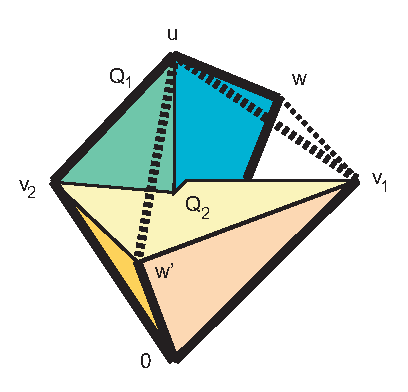
\includegraphics{\ps/isolatedpair.eps}
  \caption{An isolated pair.  The isolated pair consists of two simplices
   $Q_1=\{0,u,w,v_2\}$ and $Q_2=\{0,w',v_1,v_2\}$.  The six extremal vertices
   form an octahedron. This is not a quartered octahedron because the edges
   $\{u,w'\}$ and $\{w,v_1\}$ have length greater than $2.51$.}
  \tlabel{fig:diag19}\usage{DCG-[4.3]{ fig:diag19}}
\end{figure}


Isolated quarters that meet in the interior with another strict
quarter do not belong to the $Q$-system.


%%

\newpage
